\documentclass[twoside]{book}

% Packages required by doxygen
\usepackage{fixltx2e}
\usepackage{calc}
\usepackage{doxygen}
\usepackage[export]{adjustbox} % also loads graphicx
\usepackage{graphicx}
\usepackage[utf8]{inputenc}
\usepackage{makeidx}
\usepackage{multicol}
\usepackage{multirow}
\PassOptionsToPackage{warn}{textcomp}
\usepackage{textcomp}
\usepackage[nointegrals]{wasysym}
\usepackage[table]{xcolor}

% Font selection
\usepackage[T1]{fontenc}
\usepackage[scaled=.90]{helvet}
\usepackage{courier}
\usepackage{amssymb}
\usepackage{sectsty}
\renewcommand{\familydefault}{\sfdefault}
\allsectionsfont{%
  \fontseries{bc}\selectfont%
  \color{darkgray}%
}
\renewcommand{\DoxyLabelFont}{%
  \fontseries{bc}\selectfont%
  \color{darkgray}%
}
\newcommand{\+}{\discretionary{\mbox{\scriptsize$\hookleftarrow$}}{}{}}

% Page & text layout
\usepackage{geometry}
\geometry{%
  a4paper,%
  top=2.5cm,%
  bottom=2.5cm,%
  left=2.5cm,%
  right=2.5cm%
}
\tolerance=750
\hfuzz=15pt
\hbadness=750
\setlength{\emergencystretch}{15pt}
\setlength{\parindent}{0cm}
\setlength{\parskip}{3ex plus 2ex minus 2ex}
\makeatletter
\renewcommand{\paragraph}{%
  \@startsection{paragraph}{4}{0ex}{-1.0ex}{1.0ex}{%
    \normalfont\normalsize\bfseries\SS@parafont%
  }%
}
\renewcommand{\subparagraph}{%
  \@startsection{subparagraph}{5}{0ex}{-1.0ex}{1.0ex}{%
    \normalfont\normalsize\bfseries\SS@subparafont%
  }%
}
\makeatother

% Headers & footers
\usepackage{fancyhdr}
\pagestyle{fancyplain}
\fancyhead[LE]{\fancyplain{}{\bfseries\thepage}}
\fancyhead[CE]{\fancyplain{}{}}
\fancyhead[RE]{\fancyplain{}{\bfseries\leftmark}}
\fancyhead[LO]{\fancyplain{}{\bfseries\rightmark}}
\fancyhead[CO]{\fancyplain{}{}}
\fancyhead[RO]{\fancyplain{}{\bfseries\thepage}}
\fancyfoot[LE]{\fancyplain{}{}}
\fancyfoot[CE]{\fancyplain{}{}}
\fancyfoot[RE]{\fancyplain{}{\bfseries\scriptsize Generated by Doxygen }}
\fancyfoot[LO]{\fancyplain{}{\bfseries\scriptsize Generated by Doxygen }}
\fancyfoot[CO]{\fancyplain{}{}}
\fancyfoot[RO]{\fancyplain{}{}}
\renewcommand{\footrulewidth}{0.4pt}
\renewcommand{\chaptermark}[1]{%
  \markboth{#1}{}%
}
\renewcommand{\sectionmark}[1]{%
  \markright{\thesection\ #1}%
}

% Indices & bibliography
\usepackage{natbib}
\usepackage[titles]{tocloft}
\setcounter{tocdepth}{3}
\setcounter{secnumdepth}{5}
\makeindex

% Hyperlinks (required, but should be loaded last)
\usepackage{ifpdf}
\ifpdf
  \usepackage[pdftex,pagebackref=true]{hyperref}
\else
  \usepackage[ps2pdf,pagebackref=true]{hyperref}
\fi
\hypersetup{%
  colorlinks=true,%
  linkcolor=blue,%
  citecolor=blue,%
  unicode%
}

% Custom commands
\newcommand{\clearemptydoublepage}{%
  \newpage{\pagestyle{empty}\cleardoublepage}%
}

\usepackage{caption}
\captionsetup{labelsep=space,justification=centering,font={bf},singlelinecheck=off,skip=4pt,position=top}

%===== C O N T E N T S =====

\begin{document}

% Titlepage & ToC
\hypersetup{pageanchor=false,
             bookmarksnumbered=true,
             pdfencoding=unicode
            }
\pagenumbering{roman}
\begin{titlepage}
\vspace*{7cm}
\begin{center}%
{\Large qsi-\/sim }\\
\vspace*{1cm}
{\large Generated by Doxygen 1.8.11}\\
\end{center}
\end{titlepage}
\clearemptydoublepage
\tableofcontents
\clearemptydoublepage
\pagenumbering{arabic}
\hypersetup{pageanchor=true}

%--- Begin generated contents ---
\chapter{qsi-\/sim}
\label{index}\hypertarget{index}{}Simulation Tool for Q\+Si\textquotesingle{}s dangling bonds. There are two proposed contributions\+: \begin{DoxyVerb}1. A CAD tool to assist in designing arrangements of dangling bonds on the surface.

2. A set of physics tools for the simulations of these arrangements.
\end{DoxyVerb}


\subsection*{Prerequisites}

\paragraph*{G\+UI}

The G\+UI is currently written in C++ and uses the Qt5 framework. The Qt5 framework will need to be installed in order to compile the source\+:


\begin{DoxyEnumerate}
\item The latest Qt5 source can be installed from \href{https://github.com/qt/qt5,}{\tt https\+://github.\+com/qt/qt5,} see their R\+E\+A\+D\+ME for build instructions.
\item Alternatively, an installer for the latest stable framework can be obtained from \href{https://www.qt.io/download/}{\tt https\+://www.\+qt.\+io/download/}. Currently, all source code for the G\+UI can fall under the G\+NU L\+G\+PL v3 license so select \char`\"{}\+Open source distribution...\char`\"{}. This may change in future.
\end{DoxyEnumerate}

Depending on your installation method, you may need to first install Qt5 dependencies. On debian systems, these can be installed as (build-\/essential, libfontconfig1, mesa-\/common-\/dev, libglu1-\/mesa-\/dev).

\subsection*{Building}

There is currently no installer binary so the tool must be built from source. Development has been done purely in Linux and there has been no modification made to the .pro file to account for any additional O\+S-\/specified linking/includes.

If you are going to load the source as a project in Qt Creator, make a copy of the .pro file before first compile to prevent including unnecessary formatting in the official version. When committing your code, move only the necessary changes into the official .pro file with comments as needed.

\subsubsection*{Ubuntu compilation}

This tutorial is based off Ubuntu 17.\+10. First, clone the repository (including submodules) onto your local machine using the following command\+:


\begin{DoxyCode}
1 git clone --recurse-submodules https://github.com/retallickj/qsi-sim.git
\end{DoxyCode}


You may be prompted for your Github credentials as this is a private repository. Next, install required dependencies\+:


\begin{DoxyCode}
1 sudo apt install python3-pip python3-tk make gcc g++ qtchooser qt5-default libqt5svg5* qttools5-dev
       qttools5-dev-tools libboost-dev libboost-filesystem-dev libboost-system-dev
2 sudo pip3 install matplotlib numpy pyqt5
\end{DoxyCode}


Next, compile the physics engines. The Marcus simulator is the exciting deal now so that will be the only one built in this tutorial. Build the A\+FM Marcus simulator\+:


\begin{DoxyCode}
1 cd qsi-sim/src/phys/afmmarcus/src
2 make
\end{DoxyCode}


Then compile the G\+UI (without sudo)\+:


\begin{DoxyCode}
1 cd ../../../..
2 qmake && make install
\end{DoxyCode}


Don\textquotesingle{}t be alarmed by the {\ttfamily make install}, this won\textquotesingle{}t install the simulator to your system as long as you don\textquotesingle{}t run it as sudo. All it does is compile the binaries and copy the physics simulation files over to the compiled folders.

Finally, run {\ttfamily ./build/debug/db-\/sim} (from the qsi-\/sim directory) to run the G\+UI. In order to run a hopping animation, create a DB layout, click on the play button on the top bar, choose the \char`\"{}\+Hopping Animator\char`\"{} engine and run. To run a line scan (which only supports one line for now, the top one), choose the \char`\"{}\+A\+F\+M Line Scan\char`\"{} engine. Test that the engine actually works by running a small layout first. If the Sim Visualize side bar appears on the right side without a pop-\/up window showing the line scan or the hopping animation, click \char`\"{}\+Show Terminal Output\char`\"{} and send Samuel the content for debugging. If you\textquotesingle{}re running a large layout (a few Q\+CA cells are already large), it might just take longer for the animation to show up.

The simulation parameters form is very barebones right now consisting of only textboxes, improvements will be made shortly. Electrode and A\+FM paths have not been fully integrated for simulation yet, they will also be added soon.

\subsection*{Licensing}

The open source version of Qt5 falls under the G\+NU L\+G\+PL v3 license, as does the G\+UI code. Qt5 includes some packages which include third-\/party content under different licenses. If these are used their specific licenses must be considered. Refer to \href{http://doc.qt.io/qt-5/licenses-used-in-qt.html}{\tt http\+://doc.\+qt.\+io/qt-\/5/licenses-\/used-\/in-\/qt.\+html} for a list of third-\/party licensed libraries.

\section*{T\+O\+DO}

\begin{quote}
content directly related to the G\+UI and not any solver or physics functionality \end{quote}
\subsection*{G\+UI}

\subsubsection*{Generic}


\begin{DoxyItemize}
\item Save DB layouts and load from save
\begin{DoxyItemize}
\item $\sim$$\sim$\+Save load script for each class$\sim$$\sim$ Implemented 17.\+08.\+09
\item $\sim$$\sim$\char`\"{}\+You have unsaved changes...\char`\"{}$\sim$$\sim$ Implemented 17.\+08.\+22
\item $\sim$$\sim$\+C-\/s C-\/\+Shift-\/s shortcuts$\sim$$\sim$ Implemented
\item $\sim$$\sim$\+Periodic autosave$\sim$$\sim$ 17.\+08.\+22
\item Autorecovery
\end{DoxyItemize}
\item Reseting design panel doesn\textquotesingle{}t reset tool type to Select
\item Don\textquotesingle{}t deselect cells when entering Panning mode
\item When using D\+B\+Gen Tool, show ghosts indicating where D\+Bs will be created
\item Labels (input, output, other arbitrary labels)
\item Screen capture tool options (light background mode, capture area)
\item C\+MI mode (e.\+g. single command to run batch simulations)
\item Shift + middle click drag \char`\"{}zoom to region\char`\"{}
\item Dialog panel add H\+T\+ML color processing (and regex remove H\+T\+ML tags when writing to log)
\item Make function that determines whether specific actions are allowed in current display mode
\item Break gui\+::\+Application\+G\+U\+I\+::save\+To\+File apart to a modular file writer, and pick what to include in the output file
\item $\sim$$\sim$\+Esc cancels paste operation$\sim$$\sim$ Implemented 17.\+07.\+13
\item $\sim$$\sim$\+Esc cancels DB Tool$\sim$$\sim$ Implemented 17.\+07.\+13
\item $\sim$$\sim$\+Visual feedback on which tool is currently in use (e.\+g. changed background of the button)$\sim$$\sim$ Implemented 17.\+07.\+12
\item Content Menu
\begin{DoxyItemize}
\item $\sim$$\sim$\+Generic Undo, Redo, Cut, Copy, Paste, Delete$\sim$$\sim$ 17.\+12.\+07
\item $\sim$$\sim$\+Dot specific\+: Toggle selected dots between Lattice\+Dot and D\+B\+Dot$\sim$$\sim$ 18.\+01.\+15
\item $\sim$$\sim$\+Electrode specific\+: Set potential value$\sim$$\sim$ 17.\+12.\+06
\end{DoxyItemize}
\end{DoxyItemize}

\subsubsection*{Layers}


\begin{DoxyItemize}
\item Layer editor updates in response to signals emitted from design panel
\begin{DoxyItemize}
\item Reset layer editor after loading new layout
\end{DoxyItemize}
\item $\sim$$\sim$\+Enumerated layer types$\sim$$\sim$ Implemented 18.\+01.\+15
\begin{DoxyItemize}
\item $\sim$$\sim$\+Provide enum to Q\+String conversion$\sim$$\sim$ 18.\+01.\+15
\item $\sim$$\sim$\+Also update save, load, export functions as the Enum strings are different from the original names$\sim$$\sim$ 18.\+01.\+15
\end{DoxyItemize}
\item A\+FM
\begin{DoxyItemize}
\item Path primitive object with snap to DB capabilities
\item Constant speed / acceleration profile / etc.
\begin{DoxyItemize}
\item Real time info of timing, etc.
\end{DoxyItemize}
\item Side view of A\+FM path allowing height adjustment and height movement profile, pop-\/up window when clicked on a segment
\end{DoxyItemize}
\item Create\+Layer with undo and redo in Design\+Panel
\item Add zheight property to layers (including updating functions in DP)
\item Layer\+Editor
\begin{DoxyItemize}
\item $\sim$$\sim$\+List layers$\sim$$\sim$ Implemented 18.\+01.\+15
\item Add layer
\item Rm layer
\item Rename layer (except for default layers)
\item $\sim$$\sim$\+Edit layer zheight$\sim$$\sim$ Implemented 18.\+01.\+16
\end{DoxyItemize}
\item Toggle layer state
\begin{DoxyItemize}
\item $\sim$$\sim$\+Layer visibility$\sim$$\sim$ Implemented 18.\+01.\+12
\item Layer editability
\begin{DoxyItemize}
\item Current \char`\"{}set\+Active()\char`\"{} in layer has not been implemented
\item Hiding a layer should also make it uneditable
\end{DoxyItemize}
\item Label visibility (labels can be stored within any layer when implemented)
\end{DoxyItemize}
\item Distinguishment between physical layer and logical layer
\begin{DoxyItemize}
\item Update code in physics engine
\end{DoxyItemize}
\end{DoxyItemize}

\subsubsection*{Aggregates}


\begin{DoxyItemize}
\item Save and load aggregates
\item Disallow creation of new dots inside aggregates
\item Offset of moving aggregates -\/ ghost should not be centered to the cursor, instead centered at the same offset as the starting point
\item Component library
\item Tight aggregate boundaries (instead of the current sqaure, taking up too much space)
\begin{DoxyItemize}
\item Multiple aggregate boundary algorithms, so we can choose the one that ensures the highest accuracy depending for the standard library.
\item Possibly implement Chan\textquotesingle{}s algorithm for faster convex hull computation
\item Right click on object to change the aggregate boundary algorithm, give out warning if they\textquotesingle{}re attempting to do this on an aggregate that came from a library
\item Associate hull computation wit changes to the aggregate rather than the \+::shape function (recomputes every time the boundary is painted/checked).
\end{DoxyItemize}
\item \char`\"{}flatten\+Aggregate\char`\"{} function\+: for each selected aggregate, for each child of that aggregate, split if an aggregate and add children to parent.
\item Enter aggregate to make changes inside the aggregate -\/ aggregate layers (like entering group in Inkscape)
\item $\sim$$\sim$\+Highlight group boundaries when mouse over aggregates$\sim$$\sim$ Implemented 17.\+07.\+12
\item $\sim$$\sim$\+Select parent aggregate when clicking on child aggregate$\sim$$\sim$ Implemented 17.\+07.\+12
\end{DoxyItemize}

\subsubsection*{Electrode Design}


\begin{DoxyItemize}
\item Side view of vertical electrode stack
\item $\sim$$\sim$\+Top view of electrode layers$\sim$$\sim$ 17.\+10.\+31
\item $\sim$$\sim$\+Creating, moving, copying, pasting, and deleting electrodes$\sim$$\sim$ 17.\+11.\+30
\item Snapping, aligning and distributing like Inkscape
\item $\sim$$\sim$\+Save/\+Load$\sim$$\sim$ 17.\+12.\+11
\item $\sim$$\sim$\+Setting potentials (individual and batch)$\sim$$\sim$ 17.\+11.\+03
\item $\sim$$\sim$\+Ghosting when moving Electrodes (individual and batch)$\sim$$\sim$
\end{DoxyItemize}

\subsubsection*{Config}


\begin{DoxyItemize}
\item Make config file paths configurable
\item User-\/friendly config file, custom functions in Q\+Settings to read from config to Q\+Setting\textquotesingle{}s own structure / writeback changed settings to user-\/readable file
\end{DoxyItemize}

\subsubsection*{Lattice}


\begin{DoxyItemize}
\item Background lattice sites -\/$>$ change to bitmap for efficiency
\item Order of a1 and a2 in get\+Lattice\+Inds matters (segfault)
\end{DoxyItemize}

\begin{quote}
solvers, physics engine, and I/O formatting \end{quote}
\subsection*{Physics Engine}


\begin{DoxyItemize}
\item Interface with solvers (standards for passing DB configuration to them, and taking results back)
\item Reset Sim\+Manager after design panel reset
\item Open new window for showing sim results
\item Custom class containing physical structure
\begin{DoxyItemize}
\item $\sim$$\sim$\+Import size and potential data for electrodes into solver$\sim$$\sim$
\item Translate size from Qt units to physical lengths
\item Add buffer region surrounding simulation area
\end{DoxyItemize}
\item Location, dimensions, etc
\begin{DoxyItemize}
\item Custom class containing properties
\end{DoxyItemize}
\item Simple estimation tool of electron distribution
\item Static or animated display of charge (like the A\+FM images)
\item Simulation visualization panel that allows users to control visualization of simulation results
\begin{DoxyItemize}
\item Control what type of result to show
\item Filter results, e.\+g. only show results with 2 electrons
\item Time control, if the simulator supports that
\item Degenerate state visualization
\item stuff like that
\end{DoxyItemize}
\item Sim\+Anneal
\begin{DoxyItemize}
\item Distance dependent hopping\+: precompute the probability of hopping from each site to any other site, put into matrix
\end{DoxyItemize}
\item Pois\+Solver
\begin{DoxyItemize}
\item $\sim$$\sim$\+Import size and potential data for electrodes into solver$\sim$$\sim$ 18.\+02.\+05
\item $\sim$$\sim$\+Translate size from Qt units to physical lengths$\sim$$\sim$ 18.\+01.\+05
\item $\sim$$\sim$\+Add buffer region surrounding simulation area$\sim$$\sim$ 18.\+01.\+05
\item $\sim$$\sim$\+Location, dimensions, etc$\sim$$\sim$ 17.\+10.\+18
\item $\sim$$\sim$\+Implement heat map/colour map support$\sim$$\sim$ 18.\+02.\+08
\item Create a UI file in Qt Designer
\item Add simulation parameter config similar to Sim\+Anneal
\end{DoxyItemize}
\end{DoxyItemize}

\begin{quote}
general bugs \end{quote}
\subsection*{Bugs}


\begin{DoxyItemize}
\item Segfault when undoing aggregates then moving dots
\item When attempting to select D\+Bs using rubberband but clicked on a D\+B/aggregate as the starting location, the object at the starting position takes the press event and rubberband fails to show
\end{DoxyItemize}

\begin{quote}
Todo list for the current branch \end{quote}
\subsection*{Ongoing}


\begin{DoxyItemize}
\item Interface with solvers (standards for passing DB configuration to them, and taking results back)
\begin{DoxyItemize}
\item Write data structure to xml
\begin{DoxyItemize}
\item Use normal save xml for now
\item In the X\+ML, add a section containing simulation parameters
\item Temperarily use an available xml parser for now, might change later (rapidxml?)
\item Material, material parameters/properties (that can be overidden by the simulator), DB locations
\item Aggregates (in the future\+: predetermined simulation parameters for aggregates can be stored)
\begin{DoxyItemize}
\item $\sim$$\sim$\+Electrode potential and size$\sim$$\sim$
\item A way to add a \char`\"{}buffer\char`\"{} region to the outer simulation boundaries.
\item Specification of potential simulation boundaries.
\item Translating the Q\+Point locations in Qt to physical locations in the simulation.
\item Ensuring that Electrodes do not overlap with each other.
\end{DoxyItemize}
\end{DoxyItemize}
\end{DoxyItemize}
\item Simple estimation tool of electron distribution
\begin{DoxyItemize}
\item Simulated annealing algorithm with 1. electron population determined by bulk-\/\+DB interaction and 2. inter-\/\+DB electron hopping.
\item Export results to file for gui to read -\/ time, charge distribution, etc
\end{DoxyItemize}
\end{DoxyItemize}

G\+UI side
\begin{DoxyItemize}
\item Get available engines
\begin{DoxyItemize}
\item Read engine properties from certain directory, properties are stored in X\+ML files
\item Simulation jobs are ran on a runtime temp directory that is structured as follows\+: \mbox{[}temp\+Dir\mbox{]}/\mbox{[}engine\+Dir\mbox{]}/\mbox{[}problem\+Dir\mbox{]}
\item For now, Sim\+Engine\+::runtime\+Temp\+Dir is hard coded to return the only physeng
\end{DoxyItemize}
\item Show simulation options
\begin{DoxyItemize}
\item Show options relevant to the selected engine
\end{DoxyItemize}
\item Problem and result files are stored in tmp
\begin{DoxyItemize}
\item Delete them when quiting program
\end{DoxyItemize}
\item Read simultion result
\begin{DoxyItemize}
\item Application\+G\+U\+I\+::read\+Sim\+Result still has many unfinished sections
\end{DoxyItemize}
\end{DoxyItemize}

The following mess was made before d-\/wave meeting, will consolidate into list above
\begin{DoxyItemize}
\item Rundown\+:
\begin{DoxyItemize}
\item Sim Setup (pick simulator, adjust simulation params)
\begin{DoxyItemize}
\item There should be flags in the simulator info X\+ML controlling what kind of params are exported.
\item Other simulation params are described in the simulator info X\+ML too I guess?
\end{DoxyItemize}
\item Run simulation, shows simulation text output
\begin{DoxyItemize}
\item X\+ML file describing the problem and parameters is saved to a specific directory that queues simulations. The binary of the simulator is called to run the simulation.
\end{DoxyItemize}
\item When simulation completes, allow users the following options\+: 1. visualize results (details of visualization, like filters and whatnot, should be handled by another widget I guess); 2. save simulation results
\begin{DoxyItemize}
\item Simulation results, corresponding params, energy levels, etc. should be stored to different classes?
\end{DoxyItemize}
\end{DoxyItemize}
\item Detect runtime error messages from the simulator and alert the user Short future\+:
\item Static or animated display of charge (like the A\+FM images)
\begin{DoxyItemize}
\item For degenerate states where the hop is of short distance? Might need to change the way the results are exported to make this easier.
\end{DoxyItemize}
\item Has a result screen that allows user to view previous results Future\+:
\item Show currently running jobs
\item For example, some jobs might be detailed simulation for small aggregates, while another crude simulation could be ongoing in the background.
\item If this widget is called from the main window while an instance of this is open, just focus such instance.
\item Assuming that sim takes a long time to run, and user makes changes to DB, when sim is complete user can open a new tab to view the results without disturbing the updated design.
\item \hyperlink{classgui_1_1DesignPanel_a559d39b09e6e02908d54dbbe79ed09d8}{gui\+::\+Design\+Panel\+::display\+Sim\+Results} to handle multiple types of simulation results that should be shown
\end{DoxyItemize}

\begin{quote}
Past T\+O\+D\+Os for implementations of major features \end{quote}
\subsection*{Past detailed T\+O\+D\+Os}

\subsubsection*{save-\/load branch}

All tasks described here contribute to save/load functionality
\begin{DoxyItemize}
\item layer id related
\begin{DoxyItemize}
\item $\sim$$\sim$\+Change items to store layer id instead of layer pointer$\sim$$\sim$ Implemented 17.\+08.\+01
\item $\sim$$\sim$\+Add functionality to change layer id stored in layers and in child items when the layer\textquotesingle{}s index changes in the stack$\sim$$\sim$ Implemented 17.\+08.\+02
\item Clean up design panel code for layer id (make it less \textquotesingle{}hacked-\/together\textquotesingle{}, get rid of unnecessary converions)
\end{DoxyItemize}
\item $\sim$$\sim$\+Undo/\+Redo stack indexing$\sim$$\sim$ Implemented 17.\+08.\+16
\begin{DoxyItemize}
\item $\sim$$\sim$\+Make base class that always increments for each item added to the stack$\sim$$\sim$ Implemented 17.\+08.\+15
\item $\sim$$\sim$\+Each item stores the undo/redo stack I\+D$\sim$$\sim$ Implemented 17.\+08.\+15
\item $\sim$$\sim$\+When autosave/manual save are performed, store the stack id at which it was performed$\sim$$\sim$ Implemented 17.\+08.\+16
\end{DoxyItemize}
\item Saving
\begin{DoxyItemize}
\item $\sim$$\sim$\+Nested saving -\/ recursive$\sim$$\sim$ Implemented 17.\+08.\+09
\item $\sim$$\sim$\+File write error handling$\sim$$\sim$ Implemented 17.\+08.\+16
\end{DoxyItemize}
\item Loading
\begin{DoxyItemize}
\item $\sim$$\sim$\+Nested loading of items -\/ recursive$\sim$$\sim$ Implemented 17.\+08.\+11
\item $\sim$$\sim$\+Load screen offset, zoom and rotation$\sim$$\sim$ Implemented 17.\+08.\+23
\item Load layers with appropriate properties
\item Error alert dialog if latdot cannot be found during dbdot generation
\item Clean up the X\+ML read write code to have a consistent style
\end{DoxyItemize}
\item $\sim$$\sim$\+Save dialog when quitting$\sim$$\sim$ Implemented 17.\+08.\+16
\item Autosaving per x minutes
\begin{DoxyItemize}
\item $\sim$$\sim$\+Detect changes in program. If no changes, don\textquotesingle{}t run autosave.$\sim$$\sim$ Implemented 17.\+08.\+15
\item $\sim$$\sim$\+Number of saves$\sim$$\sim$ Implemented 17.\+08.\+16
\item $\sim$$\sim$\+Rotational save in a folder dedicated to that program instance$\sim$$\sim$ Implemented 17.\+08.\+16
\item Put tmp directory to system tmp?
\item Delete autosaves when quiting the program gracefully
\end{DoxyItemize}
\item autorecovery
\begin{DoxyItemize}
\item Check for existing autosaves, ask the user whether they want to recover the latest autosave.
\end{DoxyItemize}
\item Code improvement
\begin{DoxyItemize}
\item Q\+Lock\+File for locking instance folder during creation
\begin{DoxyItemize}
\item Or, get the process ID and use that as part of the directory name -\/ Q\+Core\+Application\+::application\+Pid() 
\end{DoxyItemize}
\end{DoxyItemize}
\end{DoxyItemize}
\chapter{Hierarchical Index}
\section{Class Hierarchy}
This inheritance list is sorted roughly, but not completely, alphabetically\+:\begin{DoxyCompactList}
\item \contentsline{section}{prim\+:\+:Agg\+Node}{\pageref{structprim_1_1AggNode}}{}
\item \contentsline{section}{prim\+:\+:Sim\+Job\+:\+:elec\+Dist}{\pageref{structprim_1_1SimJob_1_1elecDist}}{}
\item \contentsline{section}{prim\+:\+:Sim\+Engine\+:\+:Expected\+Sim\+Param}{\pageref{structprim_1_1SimEngine_1_1ExpectedSimParam}}{}
\item \contentsline{section}{gui\+:\+:Layer\+Editor\+:\+:Layer\+Table\+Row\+Content}{\pageref{structgui_1_1LayerEditor_1_1LayerTableRowContent}}{}
\item \contentsline{section}{prim\+:\+:Sim\+Job\+:\+:Line\+Scan\+Path}{\pageref{structprim_1_1SimJob_1_1LineScanPath}}{}
\item Q\+Graphics\+Item\begin{DoxyCompactList}
\item \contentsline{section}{prim\+:\+:Item}{\pageref{classprim_1_1Item}}{}
\begin{DoxyCompactList}
\item \contentsline{section}{prim\+:\+:A\+F\+M\+Node}{\pageref{classprim_1_1AFMNode}}{}
\item \contentsline{section}{prim\+:\+:A\+F\+M\+Path}{\pageref{classprim_1_1AFMPath}}{}
\item \contentsline{section}{prim\+:\+:A\+F\+M\+Seg}{\pageref{classprim_1_1AFMSeg}}{}
\item \contentsline{section}{prim\+:\+:Aggregate}{\pageref{classprim_1_1Aggregate}}{}
\item \contentsline{section}{prim\+:\+:D\+B\+Dot}{\pageref{classprim_1_1DBDot}}{}
\item \contentsline{section}{prim\+:\+:Electrode}{\pageref{classprim_1_1Electrode}}{}
\item \contentsline{section}{prim\+:\+:Ghost}{\pageref{classprim_1_1Ghost}}{}
\item \contentsline{section}{prim\+:\+:Ghost\+Box}{\pageref{classprim_1_1GhostBox}}{}
\item \contentsline{section}{prim\+:\+:Ghost\+Dot}{\pageref{classprim_1_1GhostDot}}{}
\item \contentsline{section}{prim\+:\+:Lattice\+Dot}{\pageref{classprim_1_1LatticeDot}}{}
\item \contentsline{section}{prim\+:\+:Pot\+Plot}{\pageref{classprim_1_1PotPlot}}{}
\end{DoxyCompactList}
\end{DoxyCompactList}
\item Q\+Graphics\+View\begin{DoxyCompactList}
\item \contentsline{section}{gui\+:\+:Design\+Panel}{\pageref{classgui_1_1DesignPanel}}{}
\end{DoxyCompactList}
\item Q\+Line\+Edit\begin{DoxyCompactList}
\item \contentsline{section}{gui\+:\+:Input\+Field}{\pageref{classgui_1_1InputField}}{}
\end{DoxyCompactList}
\item Q\+Main\+Window\begin{DoxyCompactList}
\item \contentsline{section}{gui\+:\+:Application\+G\+UI}{\pageref{classgui_1_1ApplicationGUI}}{}
\end{DoxyCompactList}
\item Q\+Object\begin{DoxyCompactList}
\item \contentsline{section}{prim\+:\+:Emitter}{\pageref{classprim_1_1Emitter}}{}
\item \contentsline{section}{prim\+:\+:Layer}{\pageref{classprim_1_1Layer}}{}
\begin{DoxyCompactList}
\item \contentsline{section}{prim\+:\+:Lattice}{\pageref{classprim_1_1Lattice}}{}
\end{DoxyCompactList}
\item \contentsline{section}{prim\+:\+:Sim\+Engine}{\pageref{classprim_1_1SimEngine}}{}
\item \contentsline{section}{prim\+:\+:Sim\+Job}{\pageref{classprim_1_1SimJob}}{}
\end{DoxyCompactList}
\item Q\+Plain\+Text\+Edit\begin{DoxyCompactList}
\item \contentsline{section}{gui\+:\+:Dialog\+Panel}{\pageref{classgui_1_1DialogPanel}}{}
\end{DoxyCompactList}
\item Q\+Reg\+Exp\+Validator\begin{DoxyCompactList}
\item \contentsline{section}{gui\+:\+:Validator}{\pageref{classgui_1_1Validator}}{}
\end{DoxyCompactList}
\item Q\+Settings\begin{DoxyCompactList}
\item \contentsline{section}{settings\+:\+:Settings}{\pageref{classsettings_1_1Settings}}{}
\begin{DoxyCompactList}
\item \contentsline{section}{settings\+:\+:App\+Settings}{\pageref{classsettings_1_1AppSettings}}{}
\item \contentsline{section}{settings\+:\+:G\+U\+I\+Settings}{\pageref{classsettings_1_1GUISettings}}{}
\item \contentsline{section}{settings\+:\+:Lattice\+Settings}{\pageref{classsettings_1_1LatticeSettings}}{}
\end{DoxyCompactList}
\end{DoxyCompactList}
\item Q\+Undo\+Command\begin{DoxyCompactList}
\item \contentsline{section}{gui\+:\+:Design\+Panel\+:\+:Create\+A\+F\+M\+Node}{\pageref{classgui_1_1DesignPanel_1_1CreateAFMNode}}{}
\item \contentsline{section}{gui\+:\+:Design\+Panel\+:\+:Create\+A\+F\+M\+Path}{\pageref{classgui_1_1DesignPanel_1_1CreateAFMPath}}{}
\item \contentsline{section}{gui\+:\+:Design\+Panel\+:\+:Create\+DB}{\pageref{classgui_1_1DesignPanel_1_1CreateDB}}{}
\item \contentsline{section}{gui\+:\+:Design\+Panel\+:\+:Create\+Electrode}{\pageref{classgui_1_1DesignPanel_1_1CreateElectrode}}{}
\item \contentsline{section}{gui\+:\+:Design\+Panel\+:\+:Create\+Pot\+Plot}{\pageref{classgui_1_1DesignPanel_1_1CreatePotPlot}}{}
\item \contentsline{section}{gui\+:\+:Design\+Panel\+:\+:Form\+Aggregate}{\pageref{classgui_1_1DesignPanel_1_1FormAggregate}}{}
\item \contentsline{section}{gui\+:\+:Design\+Panel\+:\+:Move\+Item}{\pageref{classgui_1_1DesignPanel_1_1MoveItem}}{}
\end{DoxyCompactList}
\item Q\+Widget\begin{DoxyCompactList}
\item \contentsline{section}{gui\+:\+:A\+F\+M\+Panel}{\pageref{classgui_1_1AFMPanel}}{}
\item \contentsline{section}{gui\+:\+:Info\+Panel}{\pageref{classgui_1_1InfoPanel}}{}
\item \contentsline{section}{gui\+:\+:Layer\+Editor}{\pageref{classgui_1_1LayerEditor}}{}
\item \contentsline{section}{gui\+:\+:Sim\+Manager}{\pageref{classgui_1_1SimManager}}{}
\item \contentsline{section}{gui\+:\+:Sim\+Visualize}{\pageref{classgui_1_1SimVisualize}}{}
\item \contentsline{section}{settings\+:\+:Settings\+Dialog}{\pageref{classsettings_1_1SettingsDialog}}{}
\end{DoxyCompactList}
\end{DoxyCompactList}

\chapter{Class Index}
\section{Class List}
Here are the classes, structs, unions and interfaces with brief descriptions\+:\begin{DoxyCompactList}
\item\contentsline{section}{\hyperlink{classprim_1_1AFMNode}{prim\+::\+A\+F\+M\+Node} }{\pageref{classprim_1_1AFMNode}}{}
\item\contentsline{section}{\hyperlink{classgui_1_1AFMPanel}{gui\+::\+A\+F\+M\+Panel} }{\pageref{classgui_1_1AFMPanel}}{}
\item\contentsline{section}{\hyperlink{classprim_1_1AFMPath}{prim\+::\+A\+F\+M\+Path} }{\pageref{classprim_1_1AFMPath}}{}
\item\contentsline{section}{\hyperlink{classprim_1_1AFMSeg}{prim\+::\+A\+F\+M\+Seg} }{\pageref{classprim_1_1AFMSeg}}{}
\item\contentsline{section}{\hyperlink{structprim_1_1AggNode}{prim\+::\+Agg\+Node} \\*Node structure for describing which sources belong to which aggregate }{\pageref{structprim_1_1AggNode}}{}
\item\contentsline{section}{\hyperlink{classprim_1_1Aggregate}{prim\+::\+Aggregate} \\*Custom class which is both derived from \hyperlink{classprim_1_1Item}{Item} and acts as a container class for collections of \hyperlink{classprim_1_1Item}{Item} objects }{\pageref{classprim_1_1Aggregate}}{}
\item\contentsline{section}{\hyperlink{classgui_1_1ApplicationGUI}{gui\+::\+Application\+G\+UI} }{\pageref{classgui_1_1ApplicationGUI}}{}
\item\contentsline{section}{\hyperlink{classsettings_1_1AppSettings}{settings\+::\+App\+Settings} }{\pageref{classsettings_1_1AppSettings}}{}
\item\contentsline{section}{\hyperlink{classgui_1_1DesignPanel_1_1CreateAFMNode}{gui\+::\+Design\+Panel\+::\+Create\+A\+F\+M\+Node} }{\pageref{classgui_1_1DesignPanel_1_1CreateAFMNode}}{}
\item\contentsline{section}{\hyperlink{classgui_1_1DesignPanel_1_1CreateAFMPath}{gui\+::\+Design\+Panel\+::\+Create\+A\+F\+M\+Path} }{\pageref{classgui_1_1DesignPanel_1_1CreateAFMPath}}{}
\item\contentsline{section}{\hyperlink{classgui_1_1DesignPanel_1_1CreateDB}{gui\+::\+Design\+Panel\+::\+Create\+DB} }{\pageref{classgui_1_1DesignPanel_1_1CreateDB}}{}
\item\contentsline{section}{\hyperlink{classgui_1_1DesignPanel_1_1CreateElectrode}{gui\+::\+Design\+Panel\+::\+Create\+Electrode} }{\pageref{classgui_1_1DesignPanel_1_1CreateElectrode}}{}
\item\contentsline{section}{\hyperlink{classgui_1_1DesignPanel_1_1CreatePotPlot}{gui\+::\+Design\+Panel\+::\+Create\+Pot\+Plot} }{\pageref{classgui_1_1DesignPanel_1_1CreatePotPlot}}{}
\item\contentsline{section}{\hyperlink{classprim_1_1DBDot}{prim\+::\+D\+B\+Dot} \\*Specific \hyperlink{classprim_1_1Item}{Item} derived class for a dangling bond on the lattice. Each dangling bond should correspond to a source lattice dot. For generality, each \hyperlink{classprim_1_1DBDot}{D\+B\+Dot} has its own physical location that will typically be the same as the source \hyperlink{classprim_1_1LatticeDot}{Lattice\+Dot} }{\pageref{classprim_1_1DBDot}}{}
\item\contentsline{section}{\hyperlink{classgui_1_1DesignPanel}{gui\+::\+Design\+Panel} \\*Highest level of the design window visualization. Contains all functionality for creating and viewing dangling bonds }{\pageref{classgui_1_1DesignPanel}}{}
\item\contentsline{section}{\hyperlink{classgui_1_1DialogPanel}{gui\+::\+Dialog\+Panel} }{\pageref{classgui_1_1DialogPanel}}{}
\item\contentsline{section}{\hyperlink{structprim_1_1SimJob_1_1elecDist}{prim\+::\+Sim\+Job\+::elec\+Dist} \\*Elec\+\_\+dists struct for showing where electrons are }{\pageref{structprim_1_1SimJob_1_1elecDist}}{}
\item\contentsline{section}{\hyperlink{classprim_1_1Electrode}{prim\+::\+Electrode} }{\pageref{classprim_1_1Electrode}}{}
\item\contentsline{section}{\hyperlink{classprim_1_1Emitter}{prim\+::\+Emitter} }{\pageref{classprim_1_1Emitter}}{}
\item\contentsline{section}{\hyperlink{structprim_1_1SimEngine_1_1ExpectedSimParam}{prim\+::\+Sim\+Engine\+::\+Expected\+Sim\+Param} \\*Types of sim params expected for this engine }{\pageref{structprim_1_1SimEngine_1_1ExpectedSimParam}}{}
\item\contentsline{section}{\hyperlink{classgui_1_1DesignPanel_1_1FormAggregate}{gui\+::\+Design\+Panel\+::\+Form\+Aggregate} }{\pageref{classgui_1_1DesignPanel_1_1FormAggregate}}{}
\item\contentsline{section}{\hyperlink{classprim_1_1Ghost}{prim\+::\+Ghost} \\*Collection of \hyperlink{classprim_1_1GhostDot}{Ghost\+Dot} and \hyperlink{classprim_1_1GhostBox}{Ghost\+Box} objects for moving Items or copy/paste, singleton }{\pageref{classprim_1_1Ghost}}{}
\item\contentsline{section}{\hyperlink{classprim_1_1GhostBox}{prim\+::\+Ghost\+Box} \\*The ghost associated with Electrodes. Used during move and previews }{\pageref{classprim_1_1GhostBox}}{}
\item\contentsline{section}{\hyperlink{classprim_1_1GhostDot}{prim\+::\+Ghost\+Dot} \\*The ghost associated with D\+B\+Dots and Lattice\+Dots. Used during move and previews }{\pageref{classprim_1_1GhostDot}}{}
\item\contentsline{section}{\hyperlink{classsettings_1_1GUISettings}{settings\+::\+G\+U\+I\+Settings} }{\pageref{classsettings_1_1GUISettings}}{}
\item\contentsline{section}{\hyperlink{classgui_1_1InfoPanel}{gui\+::\+Info\+Panel} }{\pageref{classgui_1_1InfoPanel}}{}
\item\contentsline{section}{\hyperlink{classgui_1_1InputField}{gui\+::\+Input\+Field} }{\pageref{classgui_1_1InputField}}{}
\item\contentsline{section}{\hyperlink{classprim_1_1Item}{prim\+::\+Item} \\*Customized Q\+Graphics\+Item subclass. All items in the Layers must inherit this class and should be distinguished by the item\+\_\+type member. Both bounding\+Rect and paint must be redefined in any derived classes }{\pageref{classprim_1_1Item}}{}
\item\contentsline{section}{\hyperlink{classprim_1_1Lattice}{prim\+::\+Lattice} }{\pageref{classprim_1_1Lattice}}{}
\item\contentsline{section}{\hyperlink{classprim_1_1LatticeDot}{prim\+::\+Lattice\+Dot} \\*Specific \hyperlink{classprim_1_1Item}{Item} derived class for showing the possible dangling bond location on the surface lattice. For now, this class has very similar characteristics to the \hyperlink{classprim_1_1DBDot}{D\+B\+Dot} but will be kept a separate class to allow for future distinction in properties and avoid overbloating the functionality of either class }{\pageref{classprim_1_1LatticeDot}}{}
\item\contentsline{section}{\hyperlink{classsettings_1_1LatticeSettings}{settings\+::\+Lattice\+Settings} }{\pageref{classsettings_1_1LatticeSettings}}{}
\item\contentsline{section}{\hyperlink{classprim_1_1Layer}{prim\+::\+Layer} \\*Base Class for design layers, layers do not delete their items when destroyed }{\pageref{classprim_1_1Layer}}{}
\item\contentsline{section}{\hyperlink{classgui_1_1LayerEditor}{gui\+::\+Layer\+Editor} }{\pageref{classgui_1_1LayerEditor}}{}
\item\contentsline{section}{\hyperlink{structgui_1_1LayerEditor_1_1LayerTableRowContent}{gui\+::\+Layer\+Editor\+::\+Layer\+Table\+Row\+Content} }{\pageref{structgui_1_1LayerEditor_1_1LayerTableRowContent}}{}
\item\contentsline{section}{\hyperlink{structprim_1_1SimJob_1_1LineScanPath}{prim\+::\+Sim\+Job\+::\+Line\+Scan\+Path} }{\pageref{structprim_1_1SimJob_1_1LineScanPath}}{}
\item\contentsline{section}{\hyperlink{classgui_1_1DesignPanel_1_1MoveItem}{gui\+::\+Design\+Panel\+::\+Move\+Item} }{\pageref{classgui_1_1DesignPanel_1_1MoveItem}}{}
\item\contentsline{section}{\hyperlink{classprim_1_1PotPlot}{prim\+::\+Pot\+Plot} \\*An item that implements a colour map of the electrostatic potential due to electrodes in the system }{\pageref{classprim_1_1PotPlot}}{}
\item\contentsline{section}{\hyperlink{classsettings_1_1Settings}{settings\+::\+Settings} }{\pageref{classsettings_1_1Settings}}{}
\item\contentsline{section}{\hyperlink{classsettings_1_1SettingsDialog}{settings\+::\+Settings\+Dialog} }{\pageref{classsettings_1_1SettingsDialog}}{}
\item\contentsline{section}{\hyperlink{classprim_1_1SimEngine}{prim\+::\+Sim\+Engine} \\*A simulation engine that can be used with the design tool }{\pageref{classprim_1_1SimEngine}}{}
\item\contentsline{section}{\hyperlink{classprim_1_1SimJob}{prim\+::\+Sim\+Job} \\*A single run of a simulation engine. Takes care of setting up simulation parameters, calling simulation engine binaries, and reading simulation results }{\pageref{classprim_1_1SimJob}}{}
\item\contentsline{section}{\hyperlink{classgui_1_1SimManager}{gui\+::\+Sim\+Manager} }{\pageref{classgui_1_1SimManager}}{}
\item\contentsline{section}{\hyperlink{classgui_1_1SimVisualize}{gui\+::\+Sim\+Visualize} }{\pageref{classgui_1_1SimVisualize}}{}
\item\contentsline{section}{\hyperlink{classgui_1_1Validator}{gui\+::\+Validator} }{\pageref{classgui_1_1Validator}}{}
\end{DoxyCompactList}

\chapter{File Index}
\section{File List}
Here is a list of all documented files with brief descriptions\+:\begin{DoxyCompactList}
\item\contentsline{section}{src/{\bfseries global.\+h} }{\pageref{global_8h}}{}
\item\contentsline{section}{src/gui/{\bfseries application.\+h} }{\pageref{application_8h}}{}
\item\contentsline{section}{src/gui/widgets/{\bfseries afm\+\_\+panel.\+h} }{\pageref{afm__panel_8h}}{}
\item\contentsline{section}{src/gui/widgets/\hyperlink{design__panel_8h}{design\+\_\+panel.\+h} \\*\+: Top level widget for the design panel. Contains all layers and functionality for reating, selecting, moving, etc. object in the design }{\pageref{design__panel_8h}}{}
\item\contentsline{section}{src/gui/widgets/\hyperlink{dialog__panel_8h}{dialog\+\_\+panel.\+h} \\*\+: Plain\+Text\+Edit field in which to display stdout when instructed }{\pageref{dialog__panel_8h}}{}
\item\contentsline{section}{src/gui/widgets/{\bfseries info\+\_\+panel.\+h} }{\pageref{info__panel_8h}}{}
\item\contentsline{section}{src/gui/widgets/{\bfseries input\+\_\+field.\+h} }{\pageref{input__field_8h}}{}
\item\contentsline{section}{src/gui/widgets/{\bfseries layer\+\_\+editor.\+h} }{\pageref{layer__editor_8h}}{}
\item\contentsline{section}{src/gui/widgets/{\bfseries sim\+\_\+manager.\+h} }{\pageref{sim__manager_8h}}{}
\item\contentsline{section}{src/gui/widgets/{\bfseries sim\+\_\+visualize\+\_\+panel.\+h} }{\pageref{sim__visualize__panel_8h}}{}
\item\contentsline{section}{src/gui/widgets/primitives/{\bfseries afmnode.\+h} }{\pageref{afmnode_8h}}{}
\item\contentsline{section}{src/gui/widgets/primitives/{\bfseries afmpath.\+h} }{\pageref{afmpath_8h}}{}
\item\contentsline{section}{src/gui/widgets/primitives/{\bfseries afmseg.\+h} }{\pageref{afmseg_8h}}{}
\item\contentsline{section}{src/gui/widgets/primitives/\hyperlink{aggregate_8h}{aggregate.\+h} \\*\+: Base class for Aggregate Item type }{\pageref{aggregate_8h}}{}
\item\contentsline{section}{src/gui/widgets/primitives/\hyperlink{dbdot_8h}{dbdot.\+h} \\*\+: D\+B\+Dot Widget for functionality of dangling bonds }{\pageref{dbdot_8h}}{}
\item\contentsline{section}{src/gui/widgets/primitives/\hyperlink{electrode_8h}{electrode.\+h} \\*\+: Function prototypes for the Electrode object }{\pageref{electrode_8h}}{}
\item\contentsline{section}{src/gui/widgets/primitives/\hyperlink{emitter_8h}{emitter.\+h} \\*\+: Assistance class Emitter which allows non Q\+Widget object to trigger an interrupt to the Design\+Widet when clicked }{\pageref{emitter_8h}}{}
\item\contentsline{section}{src/gui/widgets/primitives/\hyperlink{ghost_8h}{ghost.\+h} \\*\+: Graphical objects for moving Items and copy/paste }{\pageref{ghost_8h}}{}
\item\contentsline{section}{src/gui/widgets/primitives/\hyperlink{item_8h}{item.\+h} \\*\+: Base classes for all graphical items with custom signals }{\pageref{item_8h}}{}
\item\contentsline{section}{src/gui/widgets/primitives/{\bfseries items.\+h} }{\pageref{items_8h}}{}
\item\contentsline{section}{src/gui/widgets/primitives/\hyperlink{latdot_8h}{latdot.\+h} }{\pageref{latdot_8h}}{}
\item\contentsline{section}{src/gui/widgets/primitives/\hyperlink{lattice_8h}{lattice.\+h} }{\pageref{lattice_8h}}{}
\item\contentsline{section}{src/gui/widgets/primitives/\hyperlink{layer_8h}{layer.\+h} }{\pageref{layer_8h}}{}
\item\contentsline{section}{src/gui/widgets/primitives/\hyperlink{pot__plot_8h}{pot\+\_\+plot.\+h} \\*\+: Function prototypes for the Pot\+Plot object }{\pageref{pot__plot_8h}}{}
\item\contentsline{section}{src/gui/widgets/primitives/{\bfseries sim\+\_\+engine.\+h} }{\pageref{sim__engine_8h}}{}
\item\contentsline{section}{src/gui/widgets/primitives/\hyperlink{sim__job_8h}{sim\+\_\+job.\+h} }{\pageref{sim__job_8h}}{}
\item\contentsline{section}{src/settings/{\bfseries settings.\+h} }{\pageref{settings_8h}}{}
\item\contentsline{section}{src/settings/{\bfseries settings\+\_\+dialog.\+h} }{\pageref{settings__dialog_8h}}{}
\end{DoxyCompactList}

\chapter{Class Documentation}
\hypertarget{classprim_1_1AFMNode}{}\section{prim\+:\+:A\+F\+M\+Node Class Reference}
\label{classprim_1_1AFMNode}\index{prim\+::\+A\+F\+M\+Node@{prim\+::\+A\+F\+M\+Node}}


Inheritance diagram for prim\+:\+:A\+F\+M\+Node\+:\nopagebreak
\begin{figure}[H]
\begin{center}
\leavevmode
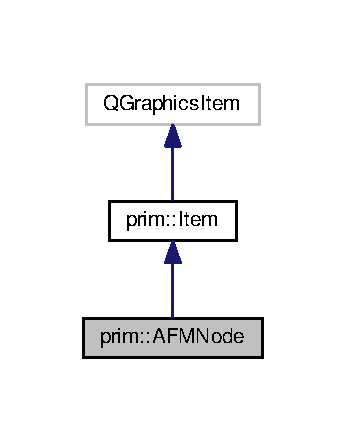
\includegraphics[width=166pt]{classprim_1_1AFMNode__inherit__graph}
\end{center}
\end{figure}


Collaboration diagram for prim\+:\+:A\+F\+M\+Node\+:\nopagebreak
\begin{figure}[H]
\begin{center}
\leavevmode
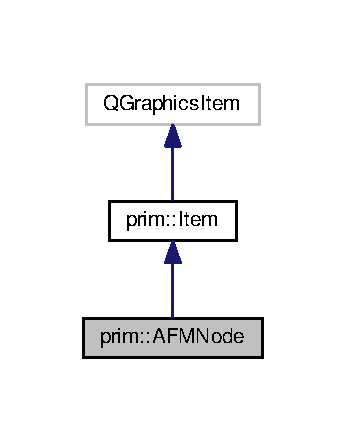
\includegraphics[width=166pt]{classprim_1_1AFMNode__coll__graph}
\end{center}
\end{figure}
\subsection*{Public Member Functions}
\begin{DoxyCompactItemize}
\item 
{\bfseries A\+F\+M\+Node} (int lay\+\_\+id, Q\+PointF scenepos, float z\+\_\+offset)\hypertarget{classprim_1_1AFMNode_adc6bf443ccb51efe21ea6bf6c77b92ef}{}\label{classprim_1_1AFMNode_adc6bf443ccb51efe21ea6bf6c77b92ef}

\item 
{\bfseries A\+F\+M\+Node} (Q\+Xml\+Stream\+Reader $\ast$rs, Q\+Graphics\+Scene $\ast$scene)\hypertarget{classprim_1_1AFMNode_a13bd3f177bf2046e5b96567a2d40970f}{}\label{classprim_1_1AFMNode_a13bd3f177bf2046e5b96567a2d40970f}

\item 
void {\bfseries init\+A\+F\+M\+Node} (int lay\+\_\+id, Q\+PointF scenepos, float z\+\_\+offset)\hypertarget{classprim_1_1AFMNode_a016c3ceff5329e9d1e90952d59429cb7}{}\label{classprim_1_1AFMNode_a016c3ceff5329e9d1e90952d59429cb7}

\item 
virtual void {\bfseries save\+Items} (Q\+Xml\+Stream\+Writer $\ast$) const \hypertarget{classprim_1_1AFMNode_ab23535932fc385ee7e0d095a4751adba}{}\label{classprim_1_1AFMNode_ab23535932fc385ee7e0d095a4751adba}

\item 
void {\bfseries set\+Z\+Offset} (float z\+\_\+offset)\hypertarget{classprim_1_1AFMNode_ad080b42722ff4f82871bd2064dec4352}{}\label{classprim_1_1AFMNode_ad080b42722ff4f82871bd2064dec4352}

\item 
float {\bfseries z\+Offset} () const \hypertarget{classprim_1_1AFMNode_a13940e18d8607133dd8f05f374a44cb5}{}\label{classprim_1_1AFMNode_a13940e18d8607133dd8f05f374a44cb5}

\item 
virtual Q\+RectF {\bfseries bounding\+Rect} () const \hypertarget{classprim_1_1AFMNode_a8dfcc69d74a0ee4a02e08b220df00a3a}{}\label{classprim_1_1AFMNode_a8dfcc69d74a0ee4a02e08b220df00a3a}

\item 
virtual void {\bfseries paint} (Q\+Painter $\ast$, const Q\+Style\+Option\+Graphics\+Item $\ast$, Q\+Widget $\ast$)\hypertarget{classprim_1_1AFMNode_a397224a3ecc82aceacaf256924b342a6}{}\label{classprim_1_1AFMNode_a397224a3ecc82aceacaf256924b342a6}

\item 
virtual \hyperlink{classprim_1_1Item}{Item} $\ast$ \hyperlink{classprim_1_1AFMNode_a5d6f53c4a6653a4a8aa2fd275b0e4302}{deep\+Copy} () const \hypertarget{classprim_1_1AFMNode_a5d6f53c4a6653a4a8aa2fd275b0e4302}{}\label{classprim_1_1AFMNode_a5d6f53c4a6653a4a8aa2fd275b0e4302}

\begin{DoxyCompactList}\small\item\em create a deep copy of the \hyperlink{classprim_1_1Item}{Item} for the clipboard. Deep-\/copied items should have no parent or scene and need only to have the information necessary to create a new copy somewhere in the scene \end{DoxyCompactList}\end{DoxyCompactItemize}
\subsection*{Public Attributes}
\begin{DoxyCompactItemize}
\item 
Q\+Color {\bfseries fill\+\_\+col}\hypertarget{classprim_1_1AFMNode_afbd02d2180f374bf8fda5c602388f0fb}{}\label{classprim_1_1AFMNode_afbd02d2180f374bf8fda5c602388f0fb}

\item 
Q\+Color {\bfseries bd\+\_\+col}\hypertarget{classprim_1_1AFMNode_afcdc6902ffbff4db7eabc679e71315c8}{}\label{classprim_1_1AFMNode_afcdc6902ffbff4db7eabc679e71315c8}

\end{DoxyCompactItemize}
\subsection*{Static Public Attributes}
\begin{DoxyCompactItemize}
\item 
static Q\+Color {\bfseries fill\+\_\+col\+\_\+default}\hypertarget{classprim_1_1AFMNode_aae20b36394bc57ec78f4f1c1e3ed2cf9}{}\label{classprim_1_1AFMNode_aae20b36394bc57ec78f4f1c1e3ed2cf9}

\item 
static Q\+Color {\bfseries fill\+\_\+col\+\_\+hovered}\hypertarget{classprim_1_1AFMNode_a12e4088c245888c13001fa6db4c61139}{}\label{classprim_1_1AFMNode_a12e4088c245888c13001fa6db4c61139}

\item 
static Q\+Color {\bfseries fill\+\_\+col\+\_\+sel}\hypertarget{classprim_1_1AFMNode_a6870910a0ee0a0b634efb714d6665eb4}{}\label{classprim_1_1AFMNode_a6870910a0ee0a0b634efb714d6665eb4}

\item 
static Q\+Color {\bfseries bd\+\_\+col\+\_\+default}\hypertarget{classprim_1_1AFMNode_a8e4868b263114fb14d5b3066c6d418cf}{}\label{classprim_1_1AFMNode_a8e4868b263114fb14d5b3066c6d418cf}

\item 
static Q\+Color {\bfseries bd\+\_\+col\+\_\+hovered}\hypertarget{classprim_1_1AFMNode_a2ab85cc5d7f630d23214b91bd5b368fa}{}\label{classprim_1_1AFMNode_a2ab85cc5d7f630d23214b91bd5b368fa}

\item 
static Q\+Color {\bfseries bd\+\_\+col\+\_\+sel}\hypertarget{classprim_1_1AFMNode_ad8bbc3690d2849c78c159c5b996fc44f}{}\label{classprim_1_1AFMNode_ad8bbc3690d2849c78c159c5b996fc44f}

\item 
static qreal {\bfseries diameter} = -\/1\hypertarget{classprim_1_1AFMNode_a15dd05c914456bc0968317a675624c72}{}\label{classprim_1_1AFMNode_a15dd05c914456bc0968317a675624c72}

\item 
static qreal {\bfseries edge\+\_\+width} = -\/1\hypertarget{classprim_1_1AFMNode_ac2896ca32cff3cd7e77eefa609e7110e}{}\label{classprim_1_1AFMNode_ac2896ca32cff3cd7e77eefa609e7110e}

\end{DoxyCompactItemize}
\subsection*{Additional Inherited Members}


The documentation for this class was generated from the following files\+:\begin{DoxyCompactItemize}
\item 
src/gui/widgets/primitives/afmnode.\+h\item 
src/gui/widgets/primitives/afmnode.\+cc\end{DoxyCompactItemize}

\hypertarget{classgui_1_1AFMPanel}{}\section{gui\+:\+:A\+F\+M\+Panel Class Reference}
\label{classgui_1_1AFMPanel}\index{gui\+::\+A\+F\+M\+Panel@{gui\+::\+A\+F\+M\+Panel}}


Inheritance diagram for gui\+:\+:A\+F\+M\+Panel\+:\nopagebreak
\begin{figure}[H]
\begin{center}
\leavevmode
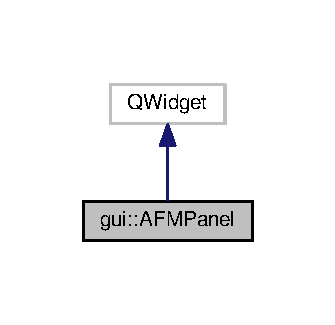
\includegraphics[width=161pt]{classgui_1_1AFMPanel__inherit__graph}
\end{center}
\end{figure}


Collaboration diagram for gui\+:\+:A\+F\+M\+Panel\+:\nopagebreak
\begin{figure}[H]
\begin{center}
\leavevmode
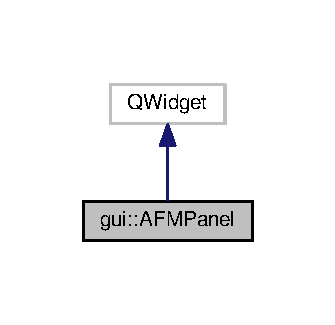
\includegraphics[width=161pt]{classgui_1_1AFMPanel__coll__graph}
\end{center}
\end{figure}
\subsection*{Public Slots}
\begin{DoxyCompactItemize}
\item 
void {\bfseries set\+Focused\+Path} (\hyperlink{classprim_1_1AFMPath}{prim\+::\+A\+F\+M\+Path} $\ast$path\+\_\+fo)\hypertarget{classgui_1_1AFMPanel_a51f99b9925a59084fb8e2ade28c7ac23}{}\label{classgui_1_1AFMPanel_a51f99b9925a59084fb8e2ade28c7ac23}

\item 
void {\bfseries set\+Focused\+Node\+Index} (int node\+\_\+ind)\hypertarget{classgui_1_1AFMPanel_a9e3546ed377fa548532b693921c0c687}{}\label{classgui_1_1AFMPanel_a9e3546ed377fa548532b693921c0c687}

\item 
void {\bfseries tool\+Change\+Response} (gui\+::\+Tool\+Type tool\+\_\+type)\hypertarget{classgui_1_1AFMPanel_a4292a6663637ca0f519286ce376524e4}{}\label{classgui_1_1AFMPanel_a4292a6663637ca0f519286ce376524e4}

\end{DoxyCompactItemize}
\subsection*{Public Member Functions}
\begin{DoxyCompactItemize}
\item 
{\bfseries A\+F\+M\+Panel} (int active\+\_\+afm\+\_\+layer\+\_\+index, Q\+Widget $\ast$parent=0)\hypertarget{classgui_1_1AFMPanel_a7132afbd429bcc6d830c7e5c83957ea7}{}\label{classgui_1_1AFMPanel_a7132afbd429bcc6d830c7e5c83957ea7}

\item 
\hyperlink{classprim_1_1AFMPath}{prim\+::\+A\+F\+M\+Path} $\ast$ {\bfseries focused\+Path} ()\hypertarget{classgui_1_1AFMPanel_a620c2f5c9e4e293faa5b4c952952be26}{}\label{classgui_1_1AFMPanel_a620c2f5c9e4e293faa5b4c952952be26}

\item 
int {\bfseries focused\+Node\+Index} ()\hypertarget{classgui_1_1AFMPanel_a32fe458af1a1714710bdf13fb954db61}{}\label{classgui_1_1AFMPanel_a32fe458af1a1714710bdf13fb954db61}

\item 
\hyperlink{classprim_1_1AFMNode}{prim\+::\+A\+F\+M\+Node} $\ast$ {\bfseries ghost\+Node} ()\hypertarget{classgui_1_1AFMPanel_a72576aaa77159369fa94bb005b394b1b}{}\label{classgui_1_1AFMPanel_a72576aaa77159369fa94bb005b394b1b}

\item 
\hyperlink{classprim_1_1AFMSeg}{prim\+::\+A\+F\+M\+Seg} $\ast$ {\bfseries ghost\+Segment} ()\hypertarget{classgui_1_1AFMPanel_a899736fb82bd6e6dc25d75f27657f26e}{}\label{classgui_1_1AFMPanel_a899736fb82bd6e6dc25d75f27657f26e}

\item 
void {\bfseries show\+Ghost} (bool)\hypertarget{classgui_1_1AFMPanel_a859d8062ef1b76db184f2ee374da19f1}{}\label{classgui_1_1AFMPanel_a859d8062ef1b76db184f2ee374da19f1}

\end{DoxyCompactItemize}


The documentation for this class was generated from the following files\+:\begin{DoxyCompactItemize}
\item 
src/gui/widgets/afm\+\_\+panel.\+h\item 
src/gui/widgets/afm\+\_\+panel.\+cc\end{DoxyCompactItemize}

\hypertarget{classprim_1_1AFMPath}{}\section{prim\+:\+:A\+F\+M\+Path Class Reference}
\label{classprim_1_1AFMPath}\index{prim\+::\+A\+F\+M\+Path@{prim\+::\+A\+F\+M\+Path}}


Inheritance diagram for prim\+:\+:A\+F\+M\+Path\+:\nopagebreak
\begin{figure}[H]
\begin{center}
\leavevmode
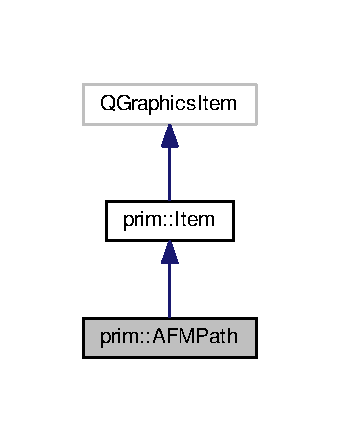
\includegraphics[width=163pt]{classprim_1_1AFMPath__inherit__graph}
\end{center}
\end{figure}


Collaboration diagram for prim\+:\+:A\+F\+M\+Path\+:\nopagebreak
\begin{figure}[H]
\begin{center}
\leavevmode
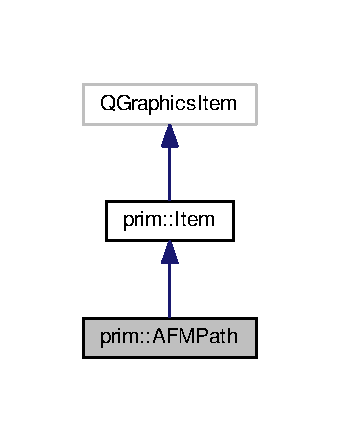
\includegraphics[width=163pt]{classprim_1_1AFMPath__coll__graph}
\end{center}
\end{figure}
\subsection*{Public Member Functions}
\begin{DoxyCompactItemize}
\item 
{\bfseries A\+F\+M\+Path} (int lay\+\_\+id)\hypertarget{classprim_1_1AFMPath_ac83ca90f162d6d97cbbc2642a0297107}{}\label{classprim_1_1AFMPath_ac83ca90f162d6d97cbbc2642a0297107}

\item 
{\bfseries A\+F\+M\+Path} (int lay\+\_\+id, const Q\+List$<$ \hyperlink{classprim_1_1AFMNode}{prim\+::\+A\+F\+M\+Node} $\ast$ $>$ \&nodes)\hypertarget{classprim_1_1AFMPath_a0ba1cedaa14e927648dd9904dc5eff2f}{}\label{classprim_1_1AFMPath_a0ba1cedaa14e927648dd9904dc5eff2f}

\item 
{\bfseries A\+F\+M\+Path} (Q\+Xml\+Stream\+Reader $\ast$rs, Q\+Graphics\+Scene $\ast$scene)\hypertarget{classprim_1_1AFMPath_a058f52115086179cc35e4de5202737ba}{}\label{classprim_1_1AFMPath_a058f52115086179cc35e4de5202737ba}

\item 
void {\bfseries init\+A\+F\+M\+Path} (int lay\+\_\+id, const Q\+List$<$ \hyperlink{classprim_1_1AFMNode}{prim\+::\+A\+F\+M\+Node} $\ast$ $>$ \&)\hypertarget{classprim_1_1AFMPath_a1a7eed6a13b583f3446652deb6791ada}{}\label{classprim_1_1AFMPath_a1a7eed6a13b583f3446652deb6791ada}

\item 
virtual void {\bfseries save\+Items} (Q\+Xml\+Stream\+Writer $\ast$) const \hypertarget{classprim_1_1AFMPath_a1d295e06021d0d0592131a49a2c0627c}{}\label{classprim_1_1AFMPath_a1d295e06021d0d0592131a49a2c0627c}

\item 
void {\bfseries insert\+Node} (\hyperlink{classprim_1_1AFMNode}{prim\+::\+A\+F\+M\+Node} $\ast$new\+\_\+node, int index=-\/1)\hypertarget{classprim_1_1AFMPath_ac4b4d5deb759bf7628f6de3934b5dae3}{}\label{classprim_1_1AFMPath_ac4b4d5deb759bf7628f6de3934b5dae3}

\item 
void {\bfseries remove\+Node} (int index)\hypertarget{classprim_1_1AFMPath_a4fb597c2b686166ebc5d3191f870d2b1}{}\label{classprim_1_1AFMPath_a4fb597c2b686166ebc5d3191f870d2b1}

\item 
\hyperlink{classprim_1_1AFMNode}{prim\+::\+A\+F\+M\+Node} $\ast$ {\bfseries get\+Node} (int index) const \hypertarget{classprim_1_1AFMPath_a21a57b453b79a8f613632f1a22b45254}{}\label{classprim_1_1AFMPath_a21a57b453b79a8f613632f1a22b45254}

\item 
\hyperlink{classprim_1_1AFMNode}{prim\+::\+A\+F\+M\+Node} $\ast$ {\bfseries get\+Last\+Node} () const \hypertarget{classprim_1_1AFMPath_a8d108e802c0a062e794cade70e5d3292}{}\label{classprim_1_1AFMPath_a8d108e802c0a062e794cade70e5d3292}

\item 
int {\bfseries get\+Node\+Index} (\hyperlink{classprim_1_1AFMNode}{prim\+::\+A\+F\+M\+Node} $\ast$node) const \hypertarget{classprim_1_1AFMPath_a75ca95fcda304a6c2ae79d8c6861fa67}{}\label{classprim_1_1AFMPath_a75ca95fcda304a6c2ae79d8c6861fa67}

\item 
int {\bfseries get\+Last\+Node\+Index} () const \hypertarget{classprim_1_1AFMPath_a6ad23059e40cd60aea15742284c85cf3}{}\label{classprim_1_1AFMPath_a6ad23059e40cd60aea15742284c85cf3}

\item 
int {\bfseries node\+Count} () const \hypertarget{classprim_1_1AFMPath_a1e4352d953ba155e599cc3403b0bb370}{}\label{classprim_1_1AFMPath_a1e4352d953ba155e599cc3403b0bb370}

\item 
int {\bfseries segment\+Count} () const \hypertarget{classprim_1_1AFMPath_aeb7a1b3a2bfb59c925a40dda4c050145}{}\label{classprim_1_1AFMPath_aeb7a1b3a2bfb59c925a40dda4c050145}

\item 
void {\bfseries insert\+Segment} (int index)\hypertarget{classprim_1_1AFMPath_abf18c50236d56de583109768a013f5ce}{}\label{classprim_1_1AFMPath_abf18c50236d56de583109768a013f5ce}

\item 
void {\bfseries remove\+Segment} (int index)\hypertarget{classprim_1_1AFMPath_ada21725f8981a80073935db0870ca1d9}{}\label{classprim_1_1AFMPath_ada21725f8981a80073935db0870ca1d9}

\item 
\hyperlink{classprim_1_1AFMSeg}{prim\+::\+A\+F\+M\+Seg} $\ast$ {\bfseries get\+Segment} (int index) const \hypertarget{classprim_1_1AFMPath_acb1b3421b2f740a8542f44978ce6f684}{}\label{classprim_1_1AFMPath_acb1b3421b2f740a8542f44978ce6f684}

\item 
Q\+List$<$ \hyperlink{classprim_1_1AFMSeg}{prim\+::\+A\+F\+M\+Seg} $\ast$ $>$ {\bfseries get\+Connected\+Segments} (\hyperlink{classprim_1_1AFMNode}{prim\+::\+A\+F\+M\+Node} $\ast$node)\hypertarget{classprim_1_1AFMPath_a1a757d57c679a56b72b01a21b84f837d}{}\label{classprim_1_1AFMPath_a1a757d57c679a56b72b01a21b84f837d}

\item 
Q\+List$<$ \hyperlink{classprim_1_1AFMSeg}{prim\+::\+A\+F\+M\+Seg} $\ast$ $>$ {\bfseries get\+Connected\+Segments} (int node\+\_\+ind)\hypertarget{classprim_1_1AFMPath_a15aec0328dc067c1cad8451341f360ff}{}\label{classprim_1_1AFMPath_a15aec0328dc067c1cad8451341f360ff}

\item 
void {\bfseries set\+Loop} (bool loop\+\_\+state)\hypertarget{classprim_1_1AFMPath_a35aea52abf0dd8f01a0cdb344372e500}{}\label{classprim_1_1AFMPath_a35aea52abf0dd8f01a0cdb344372e500}

\item 
Q\+List$<$ Q\+PointF $>$ {\bfseries unfolded\+Path} ()\hypertarget{classprim_1_1AFMPath_ab65afe23045cf5b49e7c04dbec3f9c96}{}\label{classprim_1_1AFMPath_ab65afe23045cf5b49e7c04dbec3f9c96}

\item 
virtual Q\+RectF {\bfseries bounding\+Rect} () const \hypertarget{classprim_1_1AFMPath_a1382a9b8f0339dac82fe5ab336951c47}{}\label{classprim_1_1AFMPath_a1382a9b8f0339dac82fe5ab336951c47}

\item 
virtual void {\bfseries paint} (Q\+Painter $\ast$, const Q\+Style\+Option\+Graphics\+Item $\ast$, Q\+Widget $\ast$)\hypertarget{classprim_1_1AFMPath_abc07a60a6fae8631aceb70a6e160b787}{}\label{classprim_1_1AFMPath_abc07a60a6fae8631aceb70a6e160b787}

\item 
virtual \hyperlink{classprim_1_1Item}{Item} $\ast$ \hyperlink{classprim_1_1AFMPath_a1a6c46fb657fd1c684704828541840db}{deep\+Copy} () const \hypertarget{classprim_1_1AFMPath_a1a6c46fb657fd1c684704828541840db}{}\label{classprim_1_1AFMPath_a1a6c46fb657fd1c684704828541840db}

\begin{DoxyCompactList}\small\item\em create a deep copy of the \hyperlink{classprim_1_1Item}{Item} for the clipboard. Deep-\/copied items should have no parent or scene and need only to have the information necessary to create a new copy somewhere in the scene \end{DoxyCompactList}\end{DoxyCompactItemize}
\subsection*{Additional Inherited Members}


The documentation for this class was generated from the following files\+:\begin{DoxyCompactItemize}
\item 
src/gui/widgets/primitives/afmpath.\+h\item 
src/gui/widgets/primitives/afmpath.\+cc\end{DoxyCompactItemize}

\hypertarget{classprim_1_1AFMSeg}{}\section{prim\+:\+:A\+F\+M\+Seg Class Reference}
\label{classprim_1_1AFMSeg}\index{prim\+::\+A\+F\+M\+Seg@{prim\+::\+A\+F\+M\+Seg}}


Inheritance diagram for prim\+:\+:A\+F\+M\+Seg\+:\nopagebreak
\begin{figure}[H]
\begin{center}
\leavevmode
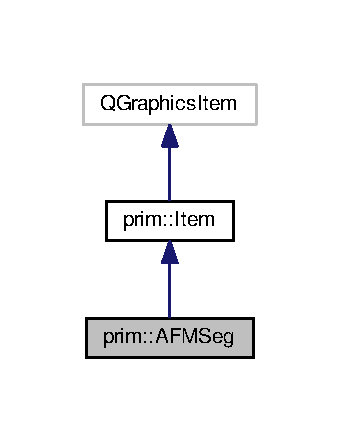
\includegraphics[width=163pt]{classprim_1_1AFMSeg__inherit__graph}
\end{center}
\end{figure}


Collaboration diagram for prim\+:\+:A\+F\+M\+Seg\+:\nopagebreak
\begin{figure}[H]
\begin{center}
\leavevmode
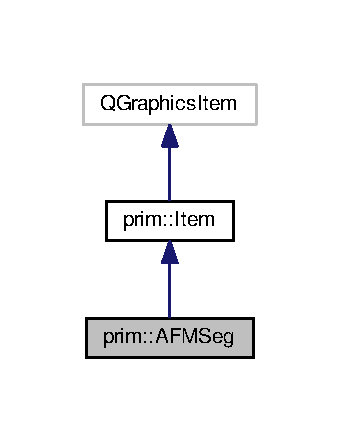
\includegraphics[width=163pt]{classprim_1_1AFMSeg__coll__graph}
\end{center}
\end{figure}
\subsection*{Public Member Functions}
\begin{DoxyCompactItemize}
\item 
{\bfseries A\+F\+M\+Seg} (int lay\+\_\+id, \hyperlink{classprim_1_1AFMNode}{prim\+::\+A\+F\+M\+Node} $\ast$orig\+\_\+node, \hyperlink{classprim_1_1AFMNode}{prim\+::\+A\+F\+M\+Node} $\ast$dest\+\_\+node)\hypertarget{classprim_1_1AFMSeg_ab42966fdda3d9cd8ff2f28cd7ff9154b}{}\label{classprim_1_1AFMSeg_ab42966fdda3d9cd8ff2f28cd7ff9154b}

\item 
{\bfseries A\+F\+M\+Seg} (Q\+Xml\+Stream\+Reader $\ast$rs, Q\+Graphics\+Scene $\ast$scene)\hypertarget{classprim_1_1AFMSeg_ab5d4f69d84cec00031a65234638f5b67}{}\label{classprim_1_1AFMSeg_ab5d4f69d84cec00031a65234638f5b67}

\item 
void {\bfseries init\+A\+F\+M\+Seg} (int lay\+\_\+id, \hyperlink{classprim_1_1AFMNode}{prim\+::\+A\+F\+M\+Node} $\ast$orig\+\_\+node, \hyperlink{classprim_1_1AFMNode}{prim\+::\+A\+F\+M\+Node} $\ast$dest\+\_\+node)\hypertarget{classprim_1_1AFMSeg_a6e149a3012c16dd8f55b3ce38d9ef46f}{}\label{classprim_1_1AFMSeg_a6e149a3012c16dd8f55b3ce38d9ef46f}

\item 
virtual void {\bfseries save\+Items} (Q\+Xml\+Stream\+Writer $\ast$) const \hypertarget{classprim_1_1AFMSeg_aacea8eed7aa86517225d6d19a9fcf4a8}{}\label{classprim_1_1AFMSeg_aacea8eed7aa86517225d6d19a9fcf4a8}

\item 
bool {\bfseries segment\+Is\+Valid} () const \hypertarget{classprim_1_1AFMSeg_afcb5e7fb168857e1b0e7bb9c6beb5648}{}\label{classprim_1_1AFMSeg_afcb5e7fb168857e1b0e7bb9c6beb5648}

\item 
void {\bfseries set\+Origin\+Node} (\hyperlink{classprim_1_1AFMNode}{prim\+::\+A\+F\+M\+Node} $\ast$orig\+\_\+node)\hypertarget{classprim_1_1AFMSeg_a13ee0fff23d20063891ba5477874f2e9}{}\label{classprim_1_1AFMSeg_a13ee0fff23d20063891ba5477874f2e9}

\item 
void {\bfseries set\+Destination\+Node} (\hyperlink{classprim_1_1AFMNode}{prim\+::\+A\+F\+M\+Node} $\ast$dest\+\_\+node)\hypertarget{classprim_1_1AFMSeg_a093f151cd938a86f8844659932d90215}{}\label{classprim_1_1AFMSeg_a093f151cd938a86f8844659932d90215}

\item 
\hyperlink{classprim_1_1AFMNode}{prim\+::\+A\+F\+M\+Node} $\ast$ {\bfseries origin\+Node} ()\hypertarget{classprim_1_1AFMSeg_a647615aa90d42be45c83064e3b329914}{}\label{classprim_1_1AFMSeg_a647615aa90d42be45c83064e3b329914}

\item 
\hyperlink{classprim_1_1AFMNode}{prim\+::\+A\+F\+M\+Node} $\ast$ {\bfseries destination\+Node} ()\hypertarget{classprim_1_1AFMSeg_ac7ff719522f14a7abee70ed32ef36474}{}\label{classprim_1_1AFMSeg_ac7ff719522f14a7abee70ed32ef36474}

\item 
void {\bfseries update\+Points} ()\hypertarget{classprim_1_1AFMSeg_a250912876820d1df7ac8345a682e4171}{}\label{classprim_1_1AFMSeg_a250912876820d1df7ac8345a682e4171}

\item 
virtual Q\+RectF {\bfseries bounding\+Rect} () const \hypertarget{classprim_1_1AFMSeg_a460f307f1f4d7b43ce31595350ebc130}{}\label{classprim_1_1AFMSeg_a460f307f1f4d7b43ce31595350ebc130}

\item 
virtual void {\bfseries paint} (Q\+Painter $\ast$, const Q\+Style\+Option\+Graphics\+Item $\ast$, Q\+Widget $\ast$)\hypertarget{classprim_1_1AFMSeg_aa066c0e229182999b5fb6b40939c2039}{}\label{classprim_1_1AFMSeg_aa066c0e229182999b5fb6b40939c2039}

\item 
virtual \hyperlink{classprim_1_1Item}{Item} $\ast$ \hyperlink{classprim_1_1AFMSeg_aa233ac610fd6ae6aeac4815b6be0e757}{deep\+Copy} () const \hypertarget{classprim_1_1AFMSeg_aa233ac610fd6ae6aeac4815b6be0e757}{}\label{classprim_1_1AFMSeg_aa233ac610fd6ae6aeac4815b6be0e757}

\begin{DoxyCompactList}\small\item\em create a deep copy of the \hyperlink{classprim_1_1Item}{Item} for the clipboard. Deep-\/copied items should have no parent or scene and need only to have the information necessary to create a new copy somewhere in the scene \end{DoxyCompactList}\end{DoxyCompactItemize}
\subsection*{Public Attributes}
\begin{DoxyCompactItemize}
\item 
Q\+Color {\bfseries fill\+\_\+col}\hypertarget{classprim_1_1AFMSeg_a279edf9d4ab5c7e18180d83e66bf25ce}{}\label{classprim_1_1AFMSeg_a279edf9d4ab5c7e18180d83e66bf25ce}

\item 
Q\+Color {\bfseries bd\+\_\+col}\hypertarget{classprim_1_1AFMSeg_a10ec279ad0f724af70490a97d1ed46e7}{}\label{classprim_1_1AFMSeg_a10ec279ad0f724af70490a97d1ed46e7}

\end{DoxyCompactItemize}
\subsection*{Static Public Attributes}
\begin{DoxyCompactItemize}
\item 
static Q\+Color {\bfseries fill\+\_\+col\+\_\+default}\hypertarget{classprim_1_1AFMSeg_a529b4b89a0ecfaa7d99ef7ed30ebee3c}{}\label{classprim_1_1AFMSeg_a529b4b89a0ecfaa7d99ef7ed30ebee3c}

\item 
static Q\+Color {\bfseries fill\+\_\+col\+\_\+hovered}\hypertarget{classprim_1_1AFMSeg_a348b6295b36b2e6626505c46ec277e2c}{}\label{classprim_1_1AFMSeg_a348b6295b36b2e6626505c46ec277e2c}

\item 
static Q\+Color {\bfseries fill\+\_\+col\+\_\+sel}\hypertarget{classprim_1_1AFMSeg_a8073a24bbdee2d9e31e34b29bc90b623}{}\label{classprim_1_1AFMSeg_a8073a24bbdee2d9e31e34b29bc90b623}

\item 
static Q\+Color {\bfseries bd\+\_\+col\+\_\+default}\hypertarget{classprim_1_1AFMSeg_a6af68fe96d65adb4f0729f4c6c25d182}{}\label{classprim_1_1AFMSeg_a6af68fe96d65adb4f0729f4c6c25d182}

\item 
static Q\+Color {\bfseries bd\+\_\+col\+\_\+hovered}\hypertarget{classprim_1_1AFMSeg_a230b904e2e45841c5ca3e138fd1d03c2}{}\label{classprim_1_1AFMSeg_a230b904e2e45841c5ca3e138fd1d03c2}

\item 
static Q\+Color {\bfseries bd\+\_\+col\+\_\+sel}\hypertarget{classprim_1_1AFMSeg_a03f6c617891b95b7481bc71f9f7a1671}{}\label{classprim_1_1AFMSeg_a03f6c617891b95b7481bc71f9f7a1671}

\item 
static qreal {\bfseries seg\+\_\+width}\hypertarget{classprim_1_1AFMSeg_aef0aacdc7deac964396aa9d2cd65cbb6}{}\label{classprim_1_1AFMSeg_aef0aacdc7deac964396aa9d2cd65cbb6}

\end{DoxyCompactItemize}
\subsection*{Additional Inherited Members}


The documentation for this class was generated from the following files\+:\begin{DoxyCompactItemize}
\item 
src/gui/widgets/primitives/afmseg.\+h\item 
src/gui/widgets/primitives/afmseg.\+cc\end{DoxyCompactItemize}

\hypertarget{structprim_1_1AggNode}{}\section{prim\+:\+:Agg\+Node Struct Reference}
\label{structprim_1_1AggNode}\index{prim\+::\+Agg\+Node@{prim\+::\+Agg\+Node}}


node structure for describing which sources belong to which aggregate  




{\ttfamily \#include $<$ghost.\+h$>$}

\subsection*{Public Types}
\begin{DoxyCompactItemize}
\item 
enum {\bfseries Source\+Type} \{ {\bfseries D\+B\+Dot}, 
{\bfseries Aggregate}, 
{\bfseries Electrode}
 \}\hypertarget{structprim_1_1AggNode_a68cd78338aa8b3429d6c4de1d3834df3}{}\label{structprim_1_1AggNode_a68cd78338aa8b3429d6c4de1d3834df3}

\end{DoxyCompactItemize}
\subsection*{Public Member Functions}
\begin{DoxyCompactItemize}
\item 
{\bfseries Agg\+Node} (int \hyperlink{structprim_1_1AggNode_a00fb2b61e32519620bb8bd6f30f79d97}{index}=-\/1)\hypertarget{structprim_1_1AggNode_adc15b91fa3513436dbec6763a087c940}{}\label{structprim_1_1AggNode_adc15b91fa3513436dbec6763a087c940}

\item 
void {\bfseries reset} ()\hypertarget{structprim_1_1AggNode_a0e1ef12a1fed11dee07e2408c9c281d6}{}\label{structprim_1_1AggNode_a0e1ef12a1fed11dee07e2408c9c281d6}

\end{DoxyCompactItemize}
\subsection*{Public Attributes}
\begin{DoxyCompactItemize}
\item 
int \hyperlink{structprim_1_1AggNode_a00fb2b61e32519620bb8bd6f30f79d97}{index}\hypertarget{structprim_1_1AggNode_a00fb2b61e32519620bb8bd6f30f79d97}{}\label{structprim_1_1AggNode_a00fb2b61e32519620bb8bd6f30f79d97}

\begin{DoxyCompactList}\small\item\em index of source if not an \hyperlink{classprim_1_1Aggregate}{Aggregate} \end{DoxyCompactList}\item 
Q\+List$<$ \hyperlink{structprim_1_1AggNode}{Agg\+Node} $\ast$ $>$ \hyperlink{structprim_1_1AggNode_a46eb56a15e6a55a9373dbbba5b364771}{nodes}\hypertarget{structprim_1_1AggNode_a46eb56a15e6a55a9373dbbba5b364771}{}\label{structprim_1_1AggNode_a46eb56a15e6a55a9373dbbba5b364771}

\begin{DoxyCompactList}\small\item\em children of the \hyperlink{classprim_1_1Aggregate}{Aggregate} if any \end{DoxyCompactList}\item 
Source\+Type {\bfseries source\+\_\+type}\hypertarget{structprim_1_1AggNode_a553e1ee04c14c6ec48bdb364d57f03fd}{}\label{structprim_1_1AggNode_a553e1ee04c14c6ec48bdb364d57f03fd}

\end{DoxyCompactItemize}


\subsection{Detailed Description}
node structure for describing which sources belong to which aggregate 

The documentation for this struct was generated from the following file\+:\begin{DoxyCompactItemize}
\item 
src/gui/widgets/primitives/\hyperlink{ghost_8h}{ghost.\+h}\end{DoxyCompactItemize}

\hypertarget{classprim_1_1Aggregate}{}\section{prim\+:\+:Aggregate Class Reference}
\label{classprim_1_1Aggregate}\index{prim\+::\+Aggregate@{prim\+::\+Aggregate}}


custom class which is both derived from \hyperlink{classprim_1_1Item}{Item} and acts as a container class for collections of \hyperlink{classprim_1_1Item}{Item} objects.  




{\ttfamily \#include $<$aggregate.\+h$>$}



Inheritance diagram for prim\+:\+:Aggregate\+:\nopagebreak
\begin{figure}[H]
\begin{center}
\leavevmode
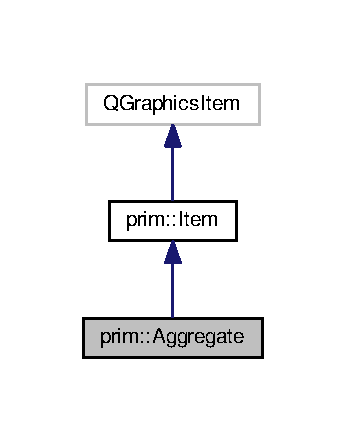
\includegraphics[width=166pt]{classprim_1_1Aggregate__inherit__graph}
\end{center}
\end{figure}


Collaboration diagram for prim\+:\+:Aggregate\+:\nopagebreak
\begin{figure}[H]
\begin{center}
\leavevmode
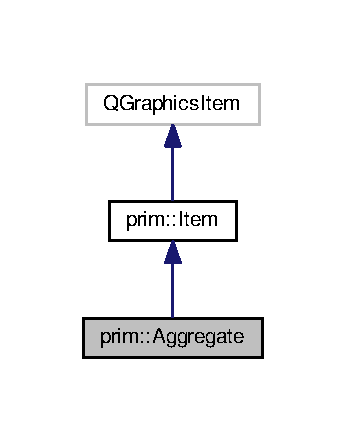
\includegraphics[width=166pt]{classprim_1_1Aggregate__coll__graph}
\end{center}
\end{figure}
\subsection*{Public Member Functions}
\begin{DoxyCompactItemize}
\item 
\hyperlink{classprim_1_1Aggregate_ac61218f83cb683de8f3d6c95eed5b510}{Aggregate} (int lay\+\_\+id, Q\+Stack$<$ \hyperlink{classprim_1_1Item}{Item} $\ast$ $>$ \&items, Q\+Graphics\+Item $\ast$parent=0)\hypertarget{classprim_1_1Aggregate_ac61218f83cb683de8f3d6c95eed5b510}{}\label{classprim_1_1Aggregate_ac61218f83cb683de8f3d6c95eed5b510}

\begin{DoxyCompactList}\small\item\em constructor, takes a list of children Items \end{DoxyCompactList}\item 
\hyperlink{classprim_1_1Aggregate_af13ccee1d00b7f611d5e46969934e461}{Aggregate} (Q\+Xml\+Stream\+Reader $\ast$stream, Q\+Graphics\+Scene $\ast$scene)\hypertarget{classprim_1_1Aggregate_af13ccee1d00b7f611d5e46969934e461}{}\label{classprim_1_1Aggregate_af13ccee1d00b7f611d5e46969934e461}

\begin{DoxyCompactList}\small\item\em constructor, creates an aggregate from the design file \end{DoxyCompactList}\item 
void {\bfseries init\+Aggregate} (Q\+Stack$<$ \hyperlink{classprim_1_1Item}{Item} $\ast$ $>$ \&items, Q\+Graphics\+Item $\ast$parent=0)\hypertarget{classprim_1_1Aggregate_ae60f489ad9a4381167c669f40779369c}{}\label{classprim_1_1Aggregate_ae60f489ad9a4381167c669f40779369c}

\item 
\hyperlink{classprim_1_1Aggregate_a8b775ab9dfdf4f8edc691ca522db45de}{$\sim$\+Aggregate} ()\hypertarget{classprim_1_1Aggregate_a8b775ab9dfdf4f8edc691ca522db45de}{}\label{classprim_1_1Aggregate_a8b775ab9dfdf4f8edc691ca522db45de}

\begin{DoxyCompactList}\small\item\em destructor, makes all children belong to Aggregates parent \end{DoxyCompactList}\item 
void \hyperlink{classprim_1_1Aggregate_a107195b0a0742ae570474c0591ef3c22}{add\+Children} (Q\+Stack$<$ \hyperlink{classprim_1_1Item}{Item} $\ast$ $>$ \&items)\hypertarget{classprim_1_1Aggregate_a107195b0a0742ae570474c0591ef3c22}{}\label{classprim_1_1Aggregate_a107195b0a0742ae570474c0591ef3c22}

\begin{DoxyCompactList}\small\item\em set given items as children \end{DoxyCompactList}\item 
Q\+Stack$<$ \hyperlink{classprim_1_1Item}{prim\+::\+Item} $\ast$ $>$ \& \hyperlink{classprim_1_1Aggregate_a348764875e84d9fb4bf169695fe9a3b9}{get\+Children} ()\hypertarget{classprim_1_1Aggregate_a348764875e84d9fb4bf169695fe9a3b9}{}\label{classprim_1_1Aggregate_a348764875e84d9fb4bf169695fe9a3b9}

\begin{DoxyCompactList}\small\item\em get all items of the aggregate \end{DoxyCompactList}\item 
virtual Q\+RectF {\bfseries bounding\+Rect} () const \hypertarget{classprim_1_1Aggregate_a9b6dce451ef2a216ac6f67376d9597a4}{}\label{classprim_1_1Aggregate_a9b6dce451ef2a216ac6f67376d9597a4}

\item 
virtual void {\bfseries paint} (Q\+Painter $\ast$, const Q\+Style\+Option\+Graphics\+Item $\ast$, Q\+Widget $\ast$)\hypertarget{classprim_1_1Aggregate_aa264a39370d3b610fca2d2b80e359a4c}{}\label{classprim_1_1Aggregate_aa264a39370d3b610fca2d2b80e359a4c}

\item 
virtual \hyperlink{classprim_1_1Item}{Item} $\ast$ \hyperlink{classprim_1_1Aggregate_ae2d55ee6f06e4aaea57bf52800a80c7a}{deep\+Copy} () const \hypertarget{classprim_1_1Aggregate_ae2d55ee6f06e4aaea57bf52800a80c7a}{}\label{classprim_1_1Aggregate_ae2d55ee6f06e4aaea57bf52800a80c7a}

\begin{DoxyCompactList}\small\item\em create a deep copy of the \hyperlink{classprim_1_1Item}{Item} for the clipboard. Deep-\/copied items should have no parent or scene and need only to have the information necessary to create a new copy somewhere in the scene \end{DoxyCompactList}\item 
virtual void {\bfseries save\+Items} (Q\+Xml\+Stream\+Writer $\ast$) const \hypertarget{classprim_1_1Aggregate_a9432adbbaa40fda61ed37b53d6237c4c}{}\label{classprim_1_1Aggregate_a9432adbbaa40fda61ed37b53d6237c4c}

\end{DoxyCompactItemize}
\subsection*{Static Public Attributes}
\begin{DoxyCompactItemize}
\item 
static Q\+Color {\bfseries edge\+\_\+col}\hypertarget{classprim_1_1Aggregate_a7c9917eb75f83ee7e89ffa8ca126d55c}{}\label{classprim_1_1Aggregate_a7c9917eb75f83ee7e89ffa8ca126d55c}

\item 
static Q\+Color {\bfseries edge\+\_\+col\+\_\+hovered}\hypertarget{classprim_1_1Aggregate_a847829d621b79311f9d234fb12a2ff1e}{}\label{classprim_1_1Aggregate_a847829d621b79311f9d234fb12a2ff1e}

\end{DoxyCompactItemize}
\subsection*{Additional Inherited Members}


\subsection{Detailed Description}
custom class which is both derived from \hyperlink{classprim_1_1Item}{Item} and acts as a container class for collections of \hyperlink{classprim_1_1Item}{Item} objects. 

The documentation for this class was generated from the following files\+:\begin{DoxyCompactItemize}
\item 
src/gui/widgets/primitives/\hyperlink{aggregate_8h}{aggregate.\+h}\item 
src/gui/widgets/primitives/aggregate.\+cc\end{DoxyCompactItemize}

\hypertarget{classgui_1_1ApplicationGUI}{}\section{gui\+:\+:Application\+G\+UI Class Reference}
\label{classgui_1_1ApplicationGUI}\index{gui\+::\+Application\+G\+UI@{gui\+::\+Application\+G\+UI}}


Inheritance diagram for gui\+:\+:Application\+G\+UI\+:\nopagebreak
\begin{figure}[H]
\begin{center}
\leavevmode
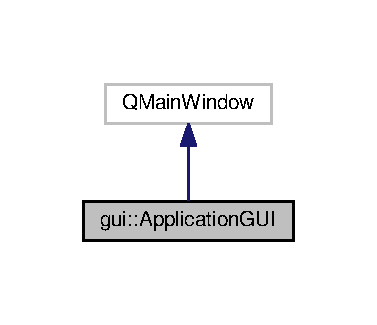
\includegraphics[width=181pt]{classgui_1_1ApplicationGUI__inherit__graph}
\end{center}
\end{figure}


Collaboration diagram for gui\+:\+:Application\+G\+UI\+:\nopagebreak
\begin{figure}[H]
\begin{center}
\leavevmode
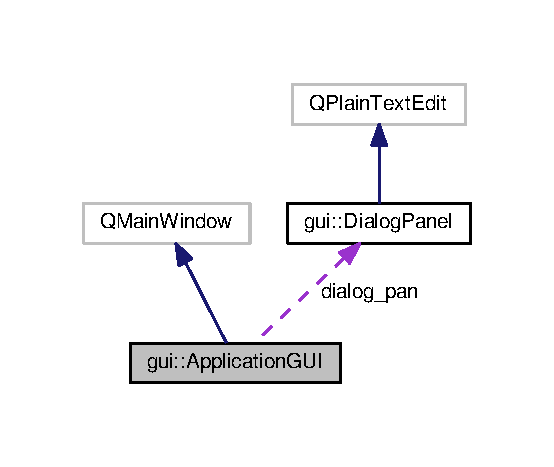
\includegraphics[width=266pt]{classgui_1_1ApplicationGUI__coll__graph}
\end{center}
\end{figure}
\subsection*{Public Types}
\begin{DoxyCompactItemize}
\item 
enum {\bfseries Save\+Flag} \{ {\bfseries Save}, 
{\bfseries Save\+As}, 
{\bfseries Auto\+Save}, 
{\bfseries Simulation}
 \}\hypertarget{classgui_1_1ApplicationGUI_a5fcaff4e236a007b986201375173c1dc}{}\label{classgui_1_1ApplicationGUI_a5fcaff4e236a007b986201375173c1dc}

\end{DoxyCompactItemize}
\subsection*{Public Slots}
\begin{DoxyCompactItemize}
\item 
void {\bfseries set\+Tool} (gui\+::\+Tool\+Type tool)\hypertarget{classgui_1_1ApplicationGUI_a5ce3df7c43609327c3463ecad2e8523f}{}\label{classgui_1_1ApplicationGUI_a5ce3df7c43609327c3463ecad2e8523f}

\item 
void {\bfseries set\+Tool\+Select} ()\hypertarget{classgui_1_1ApplicationGUI_a1c559fa2572529342acdb22e224057bf}{}\label{classgui_1_1ApplicationGUI_a1c559fa2572529342acdb22e224057bf}

\item 
void {\bfseries set\+Tool\+Drag} ()\hypertarget{classgui_1_1ApplicationGUI_ada2e3ed86aed62b24b743657fa8bb69c}{}\label{classgui_1_1ApplicationGUI_ada2e3ed86aed62b24b743657fa8bb69c}

\item 
void {\bfseries set\+Tool\+D\+B\+Gen} ()\hypertarget{classgui_1_1ApplicationGUI_a342ae32e3f77cbc535bf7cc387259328}{}\label{classgui_1_1ApplicationGUI_a342ae32e3f77cbc535bf7cc387259328}

\item 
void {\bfseries set\+Tool\+Electrode} ()\hypertarget{classgui_1_1ApplicationGUI_af13cef616153508f53cbd0f5d61849b3}{}\label{classgui_1_1ApplicationGUI_af13cef616153508f53cbd0f5d61849b3}

\item 
void {\bfseries set\+Tool\+A\+F\+M\+Path} ()\hypertarget{classgui_1_1ApplicationGUI_ae5c3980f2fa3c142f92247c147a0a5ae}{}\label{classgui_1_1ApplicationGUI_ae5c3980f2fa3c142f92247c147a0a5ae}

\item 
void {\bfseries change\+Lattice} ()\hypertarget{classgui_1_1ApplicationGUI_a23c72524cb3ddd734fd574981407c498}{}\label{classgui_1_1ApplicationGUI_a23c72524cb3ddd734fd574981407c498}

\item 
void {\bfseries parse\+Input\+Field} ()\hypertarget{classgui_1_1ApplicationGUI_a5d38e6c0dae898bb102a47ea01670299}{}\label{classgui_1_1ApplicationGUI_a5d38e6c0dae898bb102a47ea01670299}

\item 
void {\bfseries design\+Panel\+Reset} ()\hypertarget{classgui_1_1ApplicationGUI_adf4c5ee6d8a4cc9c1c46f1edb7889464}{}\label{classgui_1_1ApplicationGUI_adf4c5ee6d8a4cc9c1c46f1edb7889464}

\item 
void {\bfseries simulation\+Setup} ()\hypertarget{classgui_1_1ApplicationGUI_a7218a1d42666cef442b588c02793191a}{}\label{classgui_1_1ApplicationGUI_a7218a1d42666cef442b588c02793191a}

\item 
void {\bfseries run\+Simulation} (\hyperlink{classprim_1_1SimJob}{prim\+::\+Sim\+Job} $\ast$job)\hypertarget{classgui_1_1ApplicationGUI_aa8789f9fc4012eb41551826bba66dc3e}{}\label{classgui_1_1ApplicationGUI_aa8789f9fc4012eb41551826bba66dc3e}

\item 
bool {\bfseries read\+Sim\+Result} (const Q\+String \&result\+\_\+path)\hypertarget{classgui_1_1ApplicationGUI_ad81c4c8396d1673b92bcd8bcd4c85556}{}\label{classgui_1_1ApplicationGUI_ad81c4c8396d1673b92bcd8bcd4c85556}

\item 
void {\bfseries select\+Color} ()\hypertarget{classgui_1_1ApplicationGUI_ad2a295acee07b639d9b91a3809914d64}{}\label{classgui_1_1ApplicationGUI_ad2a295acee07b639d9b91a3809914d64}

\item 
void {\bfseries screenshot} ()\hypertarget{classgui_1_1ApplicationGUI_a5e25086665a4e1b5e4b53260dd275296}{}\label{classgui_1_1ApplicationGUI_a5e25086665a4e1b5e4b53260dd275296}

\item 
void {\bfseries design\+Screenshot} ()\hypertarget{classgui_1_1ApplicationGUI_a6b9cd8f04658f3cd4e2bf74961233364}{}\label{classgui_1_1ApplicationGUI_a6b9cd8f04658f3cd4e2bf74961233364}

\item 
void {\bfseries show\+Settings\+Dialog} ()\hypertarget{classgui_1_1ApplicationGUI_a1b66986bd5640a30a31ebcd49f6f0e0b}{}\label{classgui_1_1ApplicationGUI_a1b66986bd5640a30a31ebcd49f6f0e0b}

\item 
bool {\bfseries resolve\+Unsaved\+Changes} ()\hypertarget{classgui_1_1ApplicationGUI_ae52d505af539f8d6ae7cede1b27e884c}{}\label{classgui_1_1ApplicationGUI_ae52d505af539f8d6ae7cede1b27e884c}

\item 
void {\bfseries new\+File} ()\hypertarget{classgui_1_1ApplicationGUI_ae5d8d38378ee2ca8adfc17ab82548f90}{}\label{classgui_1_1ApplicationGUI_ae5d8d38378ee2ca8adfc17ab82548f90}

\item 
bool {\bfseries save\+To\+File} (Save\+Flag flag=Save, const Q\+String \&path=Q\+String(), \hyperlink{classprim_1_1SimJob}{prim\+::\+Sim\+Job} $\ast$sim\+\_\+job=0)\hypertarget{classgui_1_1ApplicationGUI_ae6da052182ac751e1d9ba58be16d9469}{}\label{classgui_1_1ApplicationGUI_ae6da052182ac751e1d9ba58be16d9469}

\item 
void {\bfseries save\+Default} ()\hypertarget{classgui_1_1ApplicationGUI_af8925c11e2a195a4a7328167883e5881}{}\label{classgui_1_1ApplicationGUI_af8925c11e2a195a4a7328167883e5881}

\item 
void {\bfseries save\+New} ()\hypertarget{classgui_1_1ApplicationGUI_aeb9947805dc4a88a9560da3efc4b4dc9}{}\label{classgui_1_1ApplicationGUI_aeb9947805dc4a88a9560da3efc4b4dc9}

\item 
void {\bfseries auto\+Save} ()\hypertarget{classgui_1_1ApplicationGUI_a9b43f01157f1eb88d6849eab8d4839c6}{}\label{classgui_1_1ApplicationGUI_a9b43f01157f1eb88d6849eab8d4839c6}

\item 
void {\bfseries open\+From\+File} ()\hypertarget{classgui_1_1ApplicationGUI_a6b933a1d0010174100f2295d37359c34}{}\label{classgui_1_1ApplicationGUI_a6b933a1d0010174100f2295d37359c34}

\item 
void {\bfseries close\+File} ()\hypertarget{classgui_1_1ApplicationGUI_ac4ff5dbc38abd72e3aa255db9bf6f530}{}\label{classgui_1_1ApplicationGUI_ac4ff5dbc38abd72e3aa255db9bf6f530}

\item 
bool {\bfseries export\+To\+Labview} ()\hypertarget{classgui_1_1ApplicationGUI_a24f6f7f8bc9825a295ab04cf7fa90f25}{}\label{classgui_1_1ApplicationGUI_a24f6f7f8bc9825a295ab04cf7fa90f25}

\item 
void {\bfseries about\+Version} ()\hypertarget{classgui_1_1ApplicationGUI_a82e2a3da2b93ab15928e24d390eab9ac}{}\label{classgui_1_1ApplicationGUI_a82e2a3da2b93ab15928e24d390eab9ac}

\end{DoxyCompactItemize}
\subsection*{Public Member Functions}
\begin{DoxyCompactItemize}
\item 
{\bfseries Application\+G\+UI} (Q\+Widget $\ast$parent=0)\hypertarget{classgui_1_1ApplicationGUI_ae1edfa7cc2d5ced117d438179cc596e9}{}\label{classgui_1_1ApplicationGUI_ae1edfa7cc2d5ced117d438179cc596e9}

\end{DoxyCompactItemize}
\subsection*{Static Public Attributes}
\begin{DoxyCompactItemize}
\item 
static \hyperlink{classgui_1_1DialogPanel}{gui\+::\+Dialog\+Panel} $\ast$ {\bfseries dialog\+\_\+pan} = 0\hypertarget{classgui_1_1ApplicationGUI_af407ffb8205393913f9f980da2d6d2ed}{}\label{classgui_1_1ApplicationGUI_af407ffb8205393913f9f980da2d6d2ed}

\end{DoxyCompactItemize}


The documentation for this class was generated from the following files\+:\begin{DoxyCompactItemize}
\item 
src/gui/application.\+h\item 
src/gui/application.\+cc\end{DoxyCompactItemize}

\hypertarget{classsettings_1_1AppSettings}{}\section{settings\+:\+:App\+Settings Class Reference}
\label{classsettings_1_1AppSettings}\index{settings\+::\+App\+Settings@{settings\+::\+App\+Settings}}


Inheritance diagram for settings\+:\+:App\+Settings\+:\nopagebreak
\begin{figure}[H]
\begin{center}
\leavevmode
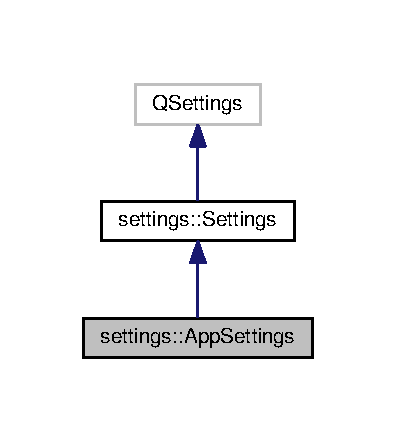
\includegraphics[width=190pt]{classsettings_1_1AppSettings__inherit__graph}
\end{center}
\end{figure}


Collaboration diagram for settings\+:\+:App\+Settings\+:\nopagebreak
\begin{figure}[H]
\begin{center}
\leavevmode
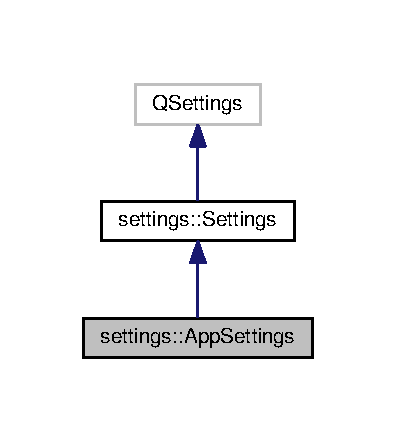
\includegraphics[width=190pt]{classsettings_1_1AppSettings__coll__graph}
\end{center}
\end{figure}
\subsection*{Static Public Member Functions}
\begin{DoxyCompactItemize}
\item 
static \hyperlink{classsettings_1_1AppSettings}{App\+Settings} $\ast$ {\bfseries instance} ()\hypertarget{classsettings_1_1AppSettings_ac17374b3cf0c542fd945dc76a3275167}{}\label{classsettings_1_1AppSettings_ac17374b3cf0c542fd945dc76a3275167}

\end{DoxyCompactItemize}
\subsection*{Additional Inherited Members}


The documentation for this class was generated from the following files\+:\begin{DoxyCompactItemize}
\item 
src/settings/settings.\+h\item 
src/settings/settings.\+cc\end{DoxyCompactItemize}

\hypertarget{classgui_1_1DesignPanel_1_1CreateAFMNode}{}\section{gui\+:\+:Design\+Panel\+:\+:Create\+A\+F\+M\+Node Class Reference}
\label{classgui_1_1DesignPanel_1_1CreateAFMNode}\index{gui\+::\+Design\+Panel\+::\+Create\+A\+F\+M\+Node@{gui\+::\+Design\+Panel\+::\+Create\+A\+F\+M\+Node}}


Inheritance diagram for gui\+:\+:Design\+Panel\+:\+:Create\+A\+F\+M\+Node\+:\nopagebreak
\begin{figure}[H]
\begin{center}
\leavevmode
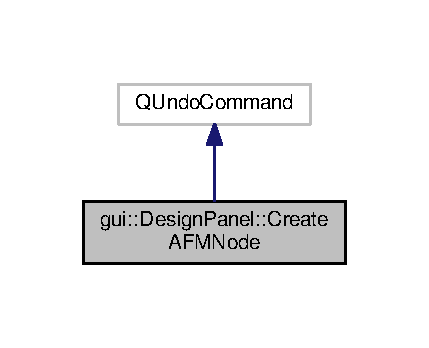
\includegraphics[width=206pt]{classgui_1_1DesignPanel_1_1CreateAFMNode__inherit__graph}
\end{center}
\end{figure}


Collaboration diagram for gui\+:\+:Design\+Panel\+:\+:Create\+A\+F\+M\+Node\+:\nopagebreak
\begin{figure}[H]
\begin{center}
\leavevmode
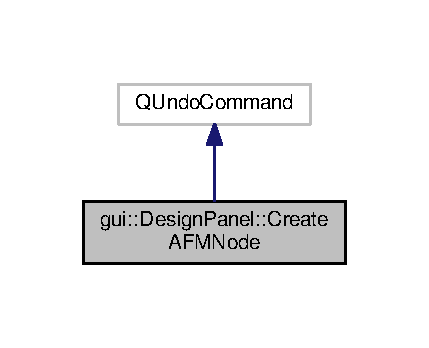
\includegraphics[width=206pt]{classgui_1_1DesignPanel_1_1CreateAFMNode__coll__graph}
\end{center}
\end{figure}
\subsection*{Public Member Functions}
\begin{DoxyCompactItemize}
\item 
{\bfseries Create\+A\+F\+M\+Node} (int layer\+\_\+index, \hyperlink{classgui_1_1DesignPanel}{Design\+Panel} $\ast$dp, Q\+PointF scenepos, float z\+\_\+offset, int afm\+\_\+index, int index\+\_\+in\+\_\+path=-\/1, bool invert=false, Q\+Undo\+Command $\ast$parent=0)\hypertarget{classgui_1_1DesignPanel_1_1CreateAFMNode_ad90c015cd6b5452d72efc4d4592bbeff}{}\label{classgui_1_1DesignPanel_1_1CreateAFMNode_ad90c015cd6b5452d72efc4d4592bbeff}

\item 
virtual void {\bfseries undo} ()\hypertarget{classgui_1_1DesignPanel_1_1CreateAFMNode_a05f5e9c036a7cce9f697965a8d345d7a}{}\label{classgui_1_1DesignPanel_1_1CreateAFMNode_a05f5e9c036a7cce9f697965a8d345d7a}

\item 
virtual void {\bfseries redo} ()\hypertarget{classgui_1_1DesignPanel_1_1CreateAFMNode_a0419aa498b760398480d4b112982d50d}{}\label{classgui_1_1DesignPanel_1_1CreateAFMNode_a0419aa498b760398480d4b112982d50d}

\end{DoxyCompactItemize}


The documentation for this class was generated from the following files\+:\begin{DoxyCompactItemize}
\item 
src/gui/widgets/\hyperlink{design__panel_8h}{design\+\_\+panel.\+h}\item 
src/gui/widgets/design\+\_\+panel.\+cc\end{DoxyCompactItemize}

\hypertarget{classgui_1_1DesignPanel_1_1CreateAFMPath}{}\section{gui\+:\+:Design\+Panel\+:\+:Create\+A\+F\+M\+Path Class Reference}
\label{classgui_1_1DesignPanel_1_1CreateAFMPath}\index{gui\+::\+Design\+Panel\+::\+Create\+A\+F\+M\+Path@{gui\+::\+Design\+Panel\+::\+Create\+A\+F\+M\+Path}}


Inheritance diagram for gui\+:\+:Design\+Panel\+:\+:Create\+A\+F\+M\+Path\+:\nopagebreak
\begin{figure}[H]
\begin{center}
\leavevmode
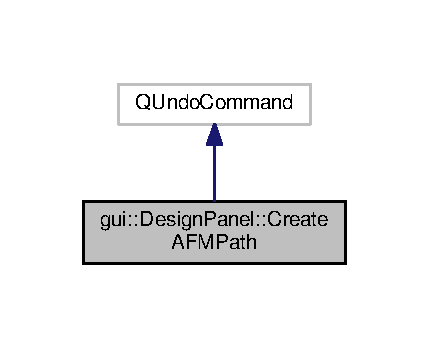
\includegraphics[width=206pt]{classgui_1_1DesignPanel_1_1CreateAFMPath__inherit__graph}
\end{center}
\end{figure}


Collaboration diagram for gui\+:\+:Design\+Panel\+:\+:Create\+A\+F\+M\+Path\+:\nopagebreak
\begin{figure}[H]
\begin{center}
\leavevmode
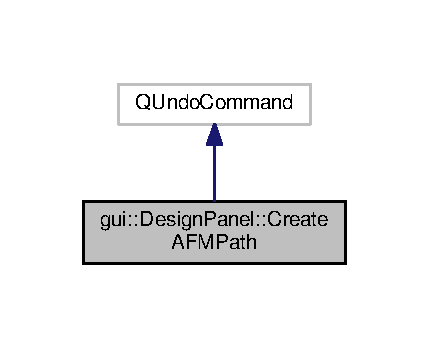
\includegraphics[width=206pt]{classgui_1_1DesignPanel_1_1CreateAFMPath__coll__graph}
\end{center}
\end{figure}
\subsection*{Public Member Functions}
\begin{DoxyCompactItemize}
\item 
{\bfseries Create\+A\+F\+M\+Path} (int layer\+\_\+index, \hyperlink{classgui_1_1DesignPanel}{Design\+Panel} $\ast$dp, \hyperlink{classprim_1_1AFMPath}{prim\+::\+A\+F\+M\+Path} $\ast$afm\+\_\+path=0, bool invert=false, Q\+Undo\+Command $\ast$parent=0)\hypertarget{classgui_1_1DesignPanel_1_1CreateAFMPath_a154cda6605b6668a1a6e47364b81bab3}{}\label{classgui_1_1DesignPanel_1_1CreateAFMPath_a154cda6605b6668a1a6e47364b81bab3}

\item 
virtual void {\bfseries undo} ()\hypertarget{classgui_1_1DesignPanel_1_1CreateAFMPath_aab5043ca7a780fcd9bef4e1b43d7a65d}{}\label{classgui_1_1DesignPanel_1_1CreateAFMPath_aab5043ca7a780fcd9bef4e1b43d7a65d}

\item 
virtual void {\bfseries redo} ()\hypertarget{classgui_1_1DesignPanel_1_1CreateAFMPath_a8a4c96b9717d9817b2636c987051cd4b}{}\label{classgui_1_1DesignPanel_1_1CreateAFMPath_a8a4c96b9717d9817b2636c987051cd4b}

\end{DoxyCompactItemize}


The documentation for this class was generated from the following files\+:\begin{DoxyCompactItemize}
\item 
src/gui/widgets/\hyperlink{design__panel_8h}{design\+\_\+panel.\+h}\item 
src/gui/widgets/design\+\_\+panel.\+cc\end{DoxyCompactItemize}

\hypertarget{classgui_1_1DesignPanel_1_1CreateDB}{}\section{gui\+:\+:Design\+Panel\+:\+:Create\+DB Class Reference}
\label{classgui_1_1DesignPanel_1_1CreateDB}\index{gui\+::\+Design\+Panel\+::\+Create\+DB@{gui\+::\+Design\+Panel\+::\+Create\+DB}}


Inheritance diagram for gui\+:\+:Design\+Panel\+:\+:Create\+DB\+:\nopagebreak
\begin{figure}[H]
\begin{center}
\leavevmode
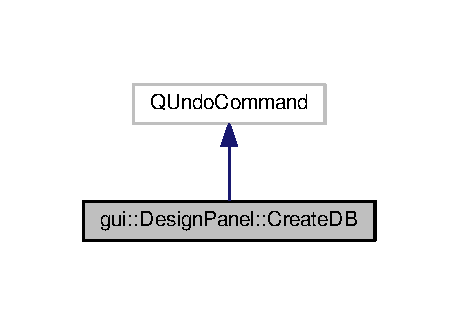
\includegraphics[width=220pt]{classgui_1_1DesignPanel_1_1CreateDB__inherit__graph}
\end{center}
\end{figure}


Collaboration diagram for gui\+:\+:Design\+Panel\+:\+:Create\+DB\+:\nopagebreak
\begin{figure}[H]
\begin{center}
\leavevmode
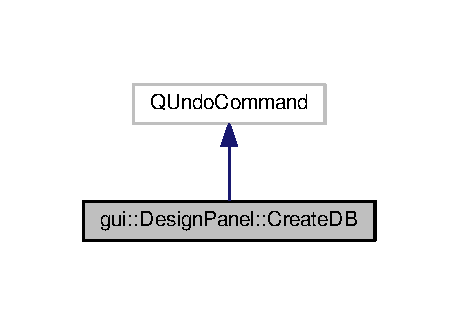
\includegraphics[width=220pt]{classgui_1_1DesignPanel_1_1CreateDB__coll__graph}
\end{center}
\end{figure}
\subsection*{Public Member Functions}
\begin{DoxyCompactItemize}
\item 
{\bfseries Create\+DB} (\hyperlink{classprim_1_1LatticeDot}{prim\+::\+Lattice\+Dot} $\ast$ldot, int layer\+\_\+index, \hyperlink{classgui_1_1DesignPanel}{Design\+Panel} $\ast$dp, \hyperlink{classprim_1_1DBDot}{prim\+::\+D\+B\+Dot} $\ast$src\+\_\+db=0, bool invert=false, Q\+Undo\+Command $\ast$parent=0)\hypertarget{classgui_1_1DesignPanel_1_1CreateDB_a208aacd117e276fe2cd4804d19dc2948}{}\label{classgui_1_1DesignPanel_1_1CreateDB_a208aacd117e276fe2cd4804d19dc2948}

\item 
virtual void {\bfseries undo} ()\hypertarget{classgui_1_1DesignPanel_1_1CreateDB_a63419aff400d1a2b1598470f28c338a5}{}\label{classgui_1_1DesignPanel_1_1CreateDB_a63419aff400d1a2b1598470f28c338a5}

\item 
virtual void {\bfseries redo} ()\hypertarget{classgui_1_1DesignPanel_1_1CreateDB_a6a830f6d5dfd02788514e99c8268b236}{}\label{classgui_1_1DesignPanel_1_1CreateDB_a6a830f6d5dfd02788514e99c8268b236}

\end{DoxyCompactItemize}


The documentation for this class was generated from the following files\+:\begin{DoxyCompactItemize}
\item 
src/gui/widgets/\hyperlink{design__panel_8h}{design\+\_\+panel.\+h}\item 
src/gui/widgets/design\+\_\+panel.\+cc\end{DoxyCompactItemize}

\hypertarget{classgui_1_1DesignPanel_1_1CreateElectrode}{}\section{gui\+:\+:Design\+Panel\+:\+:Create\+Electrode Class Reference}
\label{classgui_1_1DesignPanel_1_1CreateElectrode}\index{gui\+::\+Design\+Panel\+::\+Create\+Electrode@{gui\+::\+Design\+Panel\+::\+Create\+Electrode}}


Inheritance diagram for gui\+:\+:Design\+Panel\+:\+:Create\+Electrode\+:\nopagebreak
\begin{figure}[H]
\begin{center}
\leavevmode
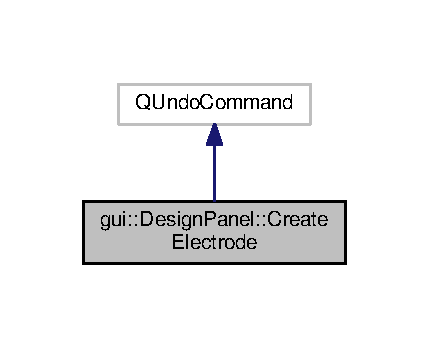
\includegraphics[width=206pt]{classgui_1_1DesignPanel_1_1CreateElectrode__inherit__graph}
\end{center}
\end{figure}


Collaboration diagram for gui\+:\+:Design\+Panel\+:\+:Create\+Electrode\+:\nopagebreak
\begin{figure}[H]
\begin{center}
\leavevmode
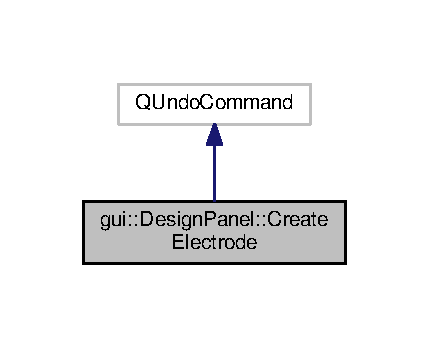
\includegraphics[width=206pt]{classgui_1_1DesignPanel_1_1CreateElectrode__coll__graph}
\end{center}
\end{figure}
\subsection*{Public Member Functions}
\begin{DoxyCompactItemize}
\item 
{\bfseries Create\+Electrode} (int layer\+\_\+index, \hyperlink{classgui_1_1DesignPanel}{gui\+::\+Design\+Panel} $\ast$dp, Q\+PointF point1, Q\+PointF point2, \hyperlink{classprim_1_1Electrode}{prim\+::\+Electrode} $\ast$elec=0, bool invert=false, Q\+Undo\+Command $\ast$parent=0)\hypertarget{classgui_1_1DesignPanel_1_1CreateElectrode_a95822013d7af2df06696360bc47d2227}{}\label{classgui_1_1DesignPanel_1_1CreateElectrode_a95822013d7af2df06696360bc47d2227}

\end{DoxyCompactItemize}


The documentation for this class was generated from the following files\+:\begin{DoxyCompactItemize}
\item 
src/gui/widgets/\hyperlink{design__panel_8h}{design\+\_\+panel.\+h}\item 
src/gui/widgets/design\+\_\+panel.\+cc\end{DoxyCompactItemize}

\hypertarget{classgui_1_1DesignPanel_1_1CreatePotPlot}{}\section{gui\+:\+:Design\+Panel\+:\+:Create\+Pot\+Plot Class Reference}
\label{classgui_1_1DesignPanel_1_1CreatePotPlot}\index{gui\+::\+Design\+Panel\+::\+Create\+Pot\+Plot@{gui\+::\+Design\+Panel\+::\+Create\+Pot\+Plot}}


Inheritance diagram for gui\+:\+:Design\+Panel\+:\+:Create\+Pot\+Plot\+:\nopagebreak
\begin{figure}[H]
\begin{center}
\leavevmode
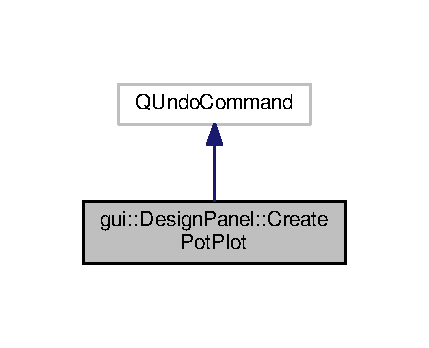
\includegraphics[width=206pt]{classgui_1_1DesignPanel_1_1CreatePotPlot__inherit__graph}
\end{center}
\end{figure}


Collaboration diagram for gui\+:\+:Design\+Panel\+:\+:Create\+Pot\+Plot\+:\nopagebreak
\begin{figure}[H]
\begin{center}
\leavevmode
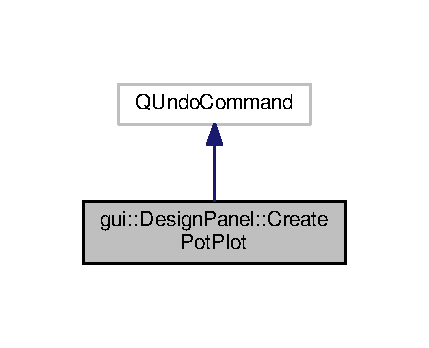
\includegraphics[width=206pt]{classgui_1_1DesignPanel_1_1CreatePotPlot__coll__graph}
\end{center}
\end{figure}
\subsection*{Public Member Functions}
\begin{DoxyCompactItemize}
\item 
{\bfseries Create\+Pot\+Plot} (int layer\+\_\+index, \hyperlink{classgui_1_1DesignPanel}{gui\+::\+Design\+Panel} $\ast$dp, Q\+Pixmap potential\+\_\+plot, Q\+RectF graph\+\_\+container, \hyperlink{classprim_1_1PotPlot}{prim\+::\+Pot\+Plot} $\ast$pp=0, bool invert=false, Q\+Undo\+Command $\ast$parent=0)\hypertarget{classgui_1_1DesignPanel_1_1CreatePotPlot_a9d19b552a75aa8c4a538ccb1b6647f2e}{}\label{classgui_1_1DesignPanel_1_1CreatePotPlot_a9d19b552a75aa8c4a538ccb1b6647f2e}

\end{DoxyCompactItemize}


The documentation for this class was generated from the following files\+:\begin{DoxyCompactItemize}
\item 
src/gui/widgets/\hyperlink{design__panel_8h}{design\+\_\+panel.\+h}\item 
src/gui/widgets/design\+\_\+panel.\+cc\end{DoxyCompactItemize}

\hypertarget{classprim_1_1DBDot}{}\section{prim\+:\+:D\+B\+Dot Class Reference}
\label{classprim_1_1DBDot}\index{prim\+::\+D\+B\+Dot@{prim\+::\+D\+B\+Dot}}


Specific \hyperlink{classprim_1_1Item}{Item} derived class for a dangling bond on the lattice. Each dangling bond should correspond to a source lattice dot. For generality, each \hyperlink{classprim_1_1DBDot}{D\+B\+Dot} has its own physical location that will typically be the same as the source \hyperlink{classprim_1_1LatticeDot}{Lattice\+Dot}.  




{\ttfamily \#include $<$dbdot.\+h$>$}



Inheritance diagram for prim\+:\+:D\+B\+Dot\+:\nopagebreak
\begin{figure}[H]
\begin{center}
\leavevmode
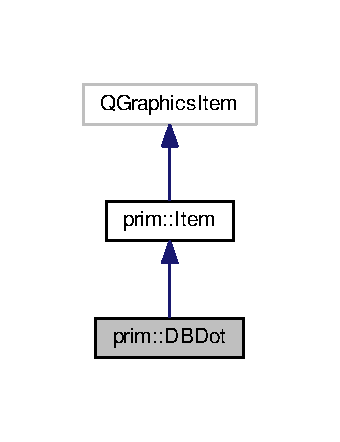
\includegraphics[width=163pt]{classprim_1_1DBDot__inherit__graph}
\end{center}
\end{figure}


Collaboration diagram for prim\+:\+:D\+B\+Dot\+:\nopagebreak
\begin{figure}[H]
\begin{center}
\leavevmode
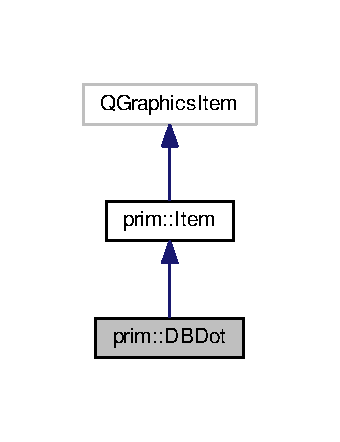
\includegraphics[width=163pt]{classprim_1_1DBDot__coll__graph}
\end{center}
\end{figure}
\subsection*{Public Member Functions}
\begin{DoxyCompactItemize}
\item 
\hyperlink{classprim_1_1DBDot_abf4a801bc53ad15aeb6b9463e223e9b2}{D\+B\+Dot} (int lay\+\_\+id, \hyperlink{classprim_1_1LatticeDot}{prim\+::\+Lattice\+Dot} $\ast$src=0, int elec\+\_\+in=0)\hypertarget{classprim_1_1DBDot_abf4a801bc53ad15aeb6b9463e223e9b2}{}\label{classprim_1_1DBDot_abf4a801bc53ad15aeb6b9463e223e9b2}

\begin{DoxyCompactList}\small\item\em constructor, creating \hyperlink{classprim_1_1DBDot}{D\+B\+Dot} using the D\+B\+Gen\+Tool. \end{DoxyCompactList}\item 
\hyperlink{classprim_1_1DBDot_acfb0c7c5503e1559c3287c2d8f2a9579}{D\+B\+Dot} (Q\+Xml\+Stream\+Reader $\ast$, Q\+Graphics\+Scene $\ast$)\hypertarget{classprim_1_1DBDot_acfb0c7c5503e1559c3287c2d8f2a9579}{}\label{classprim_1_1DBDot_acfb0c7c5503e1559c3287c2d8f2a9579}

\begin{DoxyCompactList}\small\item\em constructor, creating \hyperlink{classprim_1_1DBDot}{D\+B\+Dot} from a design file. \end{DoxyCompactList}\item 
void {\bfseries init\+D\+B\+Dot} (int lay\+\_\+id, \hyperlink{classprim_1_1LatticeDot}{prim\+::\+Lattice\+Dot} $\ast$src=0, int elec\+\_\+in=0)\hypertarget{classprim_1_1DBDot_a47fe9dc50d797d35a2cb48dd4ca512d1}{}\label{classprim_1_1DBDot_a47fe9dc50d797d35a2cb48dd4ca512d1}

\item 
Q\+PointF {\bfseries get\+Phys\+Loc} () const \hypertarget{classprim_1_1DBDot_aa4bdc68527c825257e42bae1ef06c299}{}\label{classprim_1_1DBDot_aa4bdc68527c825257e42bae1ef06c299}

\item 
void \hyperlink{classprim_1_1DBDot_afbb7f014b561e3b75b9b1d81dee4833c}{toggle\+Elec} ()\hypertarget{classprim_1_1DBDot_afbb7f014b561e3b75b9b1d81dee4833c}{}\label{classprim_1_1DBDot_afbb7f014b561e3b75b9b1d81dee4833c}

\begin{DoxyCompactList}\small\item\em Toggle between occupied and unoccupied. \end{DoxyCompactList}\item 
void \hyperlink{classprim_1_1DBDot_a9b3da606577dc4a76aabf18e4a064bb6}{set\+Elec} (int e\+\_\+in)\hypertarget{classprim_1_1DBDot_a9b3da606577dc4a76aabf18e4a064bb6}{}\label{classprim_1_1DBDot_a9b3da606577dc4a76aabf18e4a064bb6}

\begin{DoxyCompactList}\small\item\em Set electron occupancy. \end{DoxyCompactList}\item 
int \hyperlink{classprim_1_1DBDot_a0cf330485eab096e564495d7420213bc}{get\+Elec} ()\hypertarget{classprim_1_1DBDot_a0cf330485eab096e564495d7420213bc}{}\label{classprim_1_1DBDot_a0cf330485eab096e564495d7420213bc}

\begin{DoxyCompactList}\small\item\em Get electron occupancy. \end{DoxyCompactList}\item 
void \hyperlink{classprim_1_1DBDot_a1ae039b78cafd8ee28b1f8f064b59b77}{set\+Show\+Elec} (int se\+\_\+in)\hypertarget{classprim_1_1DBDot_a1ae039b78cafd8ee28b1f8f064b59b77}{}\label{classprim_1_1DBDot_a1ae039b78cafd8ee28b1f8f064b59b77}

\begin{DoxyCompactList}\small\item\em Set electron occupant visibility. \end{DoxyCompactList}\item 
void \hyperlink{classprim_1_1DBDot_a7eaa80cc7a9eef5f1b5d866393cf5071}{set\+Source} (\hyperlink{classprim_1_1LatticeDot}{prim\+::\+Lattice\+Dot} $\ast$src)\hypertarget{classprim_1_1DBDot_a7eaa80cc7a9eef5f1b5d866393cf5071}{}\label{classprim_1_1DBDot_a7eaa80cc7a9eef5f1b5d866393cf5071}

\begin{DoxyCompactList}\small\item\em Set the \hyperlink{classprim_1_1DBDot}{D\+B\+Dot} source as src, and update phys\+\_\+loc to that of src. \end{DoxyCompactList}\item 
\hyperlink{classprim_1_1LatticeDot}{prim\+::\+Lattice\+Dot} $\ast$ \hyperlink{classprim_1_1DBDot_ac9a25ede31a8741b560f2f977c26f58d}{get\+Source} () const \hypertarget{classprim_1_1DBDot_ac9a25ede31a8741b560f2f977c26f58d}{}\label{classprim_1_1DBDot_ac9a25ede31a8741b560f2f977c26f58d}

\begin{DoxyCompactList}\small\item\em Get the \hyperlink{classprim_1_1DBDot}{D\+B\+Dot} source. \end{DoxyCompactList}\item 
void {\bfseries set\+Fill} (float fill)\hypertarget{classprim_1_1DBDot_a4f87ecc0589fa5eb3c7065e776b63477}{}\label{classprim_1_1DBDot_a4f87ecc0589fa5eb3c7065e776b63477}

\item 
void {\bfseries set\+Fill\+Col} (Q\+Color col, Q\+Color col\+\_\+sel)\hypertarget{classprim_1_1DBDot_a7808bfd2be17d3ef52f950d877bda4b1}{}\label{classprim_1_1DBDot_a7808bfd2be17d3ef52f950d877bda4b1}

\item 
Q\+RectF {\bfseries bounding\+Rect} () const Q\+\_\+\+D\+E\+C\+L\+\_\+\+O\+V\+E\+R\+R\+I\+DE\hypertarget{classprim_1_1DBDot_a4ee820c9566c8de80bd41456cb1c1461}{}\label{classprim_1_1DBDot_a4ee820c9566c8de80bd41456cb1c1461}

\item 
void {\bfseries paint} (Q\+Painter $\ast$, const Q\+Style\+Option\+Graphics\+Item $\ast$, Q\+Widget $\ast$) Q\+\_\+\+D\+E\+C\+L\+\_\+\+O\+V\+E\+R\+R\+I\+DE\hypertarget{classprim_1_1DBDot_add84a5f6ceecb3312d4f7f9501528ce6}{}\label{classprim_1_1DBDot_add84a5f6ceecb3312d4f7f9501528ce6}

\item 
\hyperlink{classprim_1_1Item}{prim\+::\+Item} $\ast$ \hyperlink{classprim_1_1DBDot_ac362bbff76cb0537708bbd43fb189114}{deep\+Copy} () const \hypertarget{classprim_1_1DBDot_ac362bbff76cb0537708bbd43fb189114}{}\label{classprim_1_1DBDot_ac362bbff76cb0537708bbd43fb189114}

\begin{DoxyCompactList}\small\item\em create a deep copy of the \hyperlink{classprim_1_1Item}{Item} for the clipboard. Deep-\/copied items should have no parent or scene and need only to have the information necessary to create a new copy somewhere in the scene \end{DoxyCompactList}\item 
virtual void {\bfseries save\+Items} (Q\+Xml\+Stream\+Writer $\ast$) const \hypertarget{classprim_1_1DBDot_a8cff2080b4b633bafe0aed9012b9325c}{}\label{classprim_1_1DBDot_a8cff2080b4b633bafe0aed9012b9325c}

\end{DoxyCompactItemize}
\subsection*{Protected Member Functions}
\begin{DoxyCompactItemize}
\item 
virtual void {\bfseries mouse\+Press\+Event} (Q\+Graphics\+Scene\+Mouse\+Event $\ast$e) Q\+\_\+\+D\+E\+C\+L\+\_\+\+O\+V\+E\+R\+R\+I\+DE\hypertarget{classprim_1_1DBDot_a9c7a8a7aeb3a1b312e4d4c5b0cb10934}{}\label{classprim_1_1DBDot_a9c7a8a7aeb3a1b312e4d4c5b0cb10934}

\end{DoxyCompactItemize}
\subsection*{Additional Inherited Members}


\subsection{Detailed Description}
Specific \hyperlink{classprim_1_1Item}{Item} derived class for a dangling bond on the lattice. Each dangling bond should correspond to a source lattice dot. For generality, each \hyperlink{classprim_1_1DBDot}{D\+B\+Dot} has its own physical location that will typically be the same as the source \hyperlink{classprim_1_1LatticeDot}{Lattice\+Dot}. 

The documentation for this class was generated from the following files\+:\begin{DoxyCompactItemize}
\item 
src/gui/widgets/primitives/\hyperlink{dbdot_8h}{dbdot.\+h}\item 
src/gui/widgets/primitives/dbdot.\+cc\end{DoxyCompactItemize}

\hypertarget{classgui_1_1DesignPanel}{}\section{gui\+:\+:Design\+Panel Class Reference}
\label{classgui_1_1DesignPanel}\index{gui\+::\+Design\+Panel@{gui\+::\+Design\+Panel}}


Highest level of the design window visualization. Contains all functionality for creating and viewing dangling bonds.  




{\ttfamily \#include $<$design\+\_\+panel.\+h$>$}



Inheritance diagram for gui\+:\+:Design\+Panel\+:\nopagebreak
\begin{figure}[H]
\begin{center}
\leavevmode
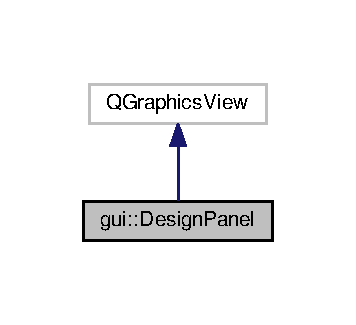
\includegraphics[width=171pt]{classgui_1_1DesignPanel__inherit__graph}
\end{center}
\end{figure}


Collaboration diagram for gui\+:\+:Design\+Panel\+:\nopagebreak
\begin{figure}[H]
\begin{center}
\leavevmode
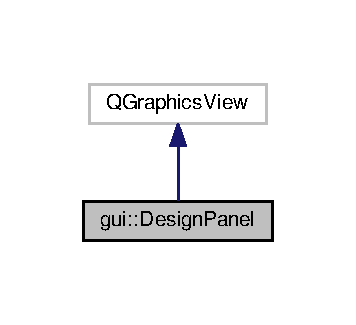
\includegraphics[width=171pt]{classgui_1_1DesignPanel__coll__graph}
\end{center}
\end{figure}
\subsection*{Classes}
\begin{DoxyCompactItemize}
\item 
class \hyperlink{classgui_1_1DesignPanel_1_1CreateAFMNode}{Create\+A\+F\+M\+Node}
\item 
class \hyperlink{classgui_1_1DesignPanel_1_1CreateAFMPath}{Create\+A\+F\+M\+Path}
\item 
class \hyperlink{classgui_1_1DesignPanel_1_1CreateDB}{Create\+DB}
\item 
class \hyperlink{classgui_1_1DesignPanel_1_1CreateElectrode}{Create\+Electrode}
\item 
class \hyperlink{classgui_1_1DesignPanel_1_1CreatePotPlot}{Create\+Pot\+Plot}
\item 
class \hyperlink{classgui_1_1DesignPanel_1_1FormAggregate}{Form\+Aggregate}
\item 
class \hyperlink{classgui_1_1DesignPanel_1_1MoveItem}{Move\+Item}
\end{DoxyCompactItemize}
\subsection*{Public Slots}
\begin{DoxyCompactItemize}
\item 
void {\bfseries select\+Clicked} (\hyperlink{classprim_1_1Item}{prim\+::\+Item} $\ast$item)\hypertarget{classgui_1_1DesignPanel_a6006a4395d7d67bb0d7f30999342a202}{}\label{classgui_1_1DesignPanel_a6006a4395d7d67bb0d7f30999342a202}

\item 
void {\bfseries sim\+Visualize\+Dock\+Visibility\+Changed} (bool visible)\hypertarget{classgui_1_1DesignPanel_ae0caa279a3ed52c4718a7039fb409c4e}{}\label{classgui_1_1DesignPanel_ae0caa279a3ed52c4718a7039fb409c4e}

\item 
void {\bfseries add\+Item\+To\+Scene\+Request} (\hyperlink{classprim_1_1Item}{prim\+::\+Item} $\ast$item)\hypertarget{classgui_1_1DesignPanel_ad69776e129c0515a72b143059472fc5f}{}\label{classgui_1_1DesignPanel_ad69776e129c0515a72b143059472fc5f}

\item 
void {\bfseries remove\+Item\+From\+Scene\+Request} (\hyperlink{classprim_1_1Item}{prim\+::\+Item} $\ast$item)\hypertarget{classgui_1_1DesignPanel_a7fd43c5342808669d9236c71e9dba741}{}\label{classgui_1_1DesignPanel_a7fd43c5342808669d9236c71e9dba741}

\item 
void {\bfseries rotate\+Cw} ()\hypertarget{classgui_1_1DesignPanel_a64662997f9df22418da01295c1f509a4}{}\label{classgui_1_1DesignPanel_a64662997f9df22418da01295c1f509a4}

\item 
void {\bfseries rotate\+Ccw} ()\hypertarget{classgui_1_1DesignPanel_a46dd4d20ad0b3ffeb42a3066e17ede81}{}\label{classgui_1_1DesignPanel_a46dd4d20ad0b3ffeb42a3066e17ede81}

\end{DoxyCompactItemize}
\subsection*{Signals}
\begin{DoxyCompactItemize}
\item 
void {\bfseries sig\+\_\+tool\+Change\+Request} (gui\+::\+Tool\+Type tool)\hypertarget{classgui_1_1DesignPanel_a8015b37634a7843a1e89b4f1a4577f0d}{}\label{classgui_1_1DesignPanel_a8015b37634a7843a1e89b4f1a4577f0d}

\item 
void {\bfseries sig\+\_\+tool\+Changed} (gui\+::\+Tool\+Type tool)\hypertarget{classgui_1_1DesignPanel_a9f7141de8ef9dc33a77286b362d1f5a0}{}\label{classgui_1_1DesignPanel_a9f7141de8ef9dc33a77286b362d1f5a0}

\item 
void {\bfseries sig\+\_\+reset\+Design\+Panel} ()\hypertarget{classgui_1_1DesignPanel_a54fdb522cee90de6f2faeabcc723e242}{}\label{classgui_1_1DesignPanel_a54fdb522cee90de6f2faeabcc723e242}

\end{DoxyCompactItemize}
\subsection*{Public Member Functions}
\begin{DoxyCompactItemize}
\item 
\hyperlink{classgui_1_1DesignPanel_a96429541df71c297fed42ae90744baf0}{Design\+Panel} (Q\+Widget $\ast$parent=0)\hypertarget{classgui_1_1DesignPanel_a96429541df71c297fed42ae90744baf0}{}\label{classgui_1_1DesignPanel_a96429541df71c297fed42ae90744baf0}

\begin{DoxyCompactList}\small\item\em constructor \end{DoxyCompactList}\item 
\hyperlink{classgui_1_1DesignPanel_aaf0992b9895822ba207eab17fd0023d9}{$\sim$\+Design\+Panel} ()\hypertarget{classgui_1_1DesignPanel_aaf0992b9895822ba207eab17fd0023d9}{}\label{classgui_1_1DesignPanel_aaf0992b9895822ba207eab17fd0023d9}

\begin{DoxyCompactList}\small\item\em destructor \end{DoxyCompactList}\item 
void \hyperlink{classgui_1_1DesignPanel_aed5d80b7651f3e25842d28f6192d4132}{init\+Design\+Panel} ()\hypertarget{classgui_1_1DesignPanel_aed5d80b7651f3e25842d28f6192d4132}{}\label{classgui_1_1DesignPanel_aed5d80b7651f3e25842d28f6192d4132}

\begin{DoxyCompactList}\small\item\em used on first init or after reset \end{DoxyCompactList}\item 
void \hyperlink{classgui_1_1DesignPanel_a5535f348b3dbcd86b15eed386b533dfc}{clear\+Design\+Panel} (bool reset=false)\hypertarget{classgui_1_1DesignPanel_a5535f348b3dbcd86b15eed386b533dfc}{}\label{classgui_1_1DesignPanel_a5535f348b3dbcd86b15eed386b533dfc}

\begin{DoxyCompactList}\small\item\em used on exit or before reset \end{DoxyCompactList}\item 
void \hyperlink{classgui_1_1DesignPanel_aa26b2b409d8f5b038270381b9eaf80cf}{reset\+Design\+Panel} ()\hypertarget{classgui_1_1DesignPanel_aa26b2b409d8f5b038270381b9eaf80cf}{}\label{classgui_1_1DesignPanel_aa26b2b409d8f5b038270381b9eaf80cf}

\begin{DoxyCompactList}\small\item\em call for reset \end{DoxyCompactList}\item 
void \hyperlink{classgui_1_1DesignPanel_a3b4be7aea300f2c35e669b06b5e6bf7e}{add\+Item} (\hyperlink{classprim_1_1Item}{prim\+::\+Item} $\ast$item, int layer\+\_\+index=-\/1, int ind=-\/1)\hypertarget{classgui_1_1DesignPanel_a3b4be7aea300f2c35e669b06b5e6bf7e}{}\label{classgui_1_1DesignPanel_a3b4be7aea300f2c35e669b06b5e6bf7e}

\begin{DoxyCompactList}\small\item\em add a new Item to the Layer at the given index of the stack. If layer\+\_\+index==-\/1, add the new item to the top\+\_\+layer. If ind != -\/1, inserts the Item into the given location of the Layer Item stack. \end{DoxyCompactList}\item 
void \hyperlink{classgui_1_1DesignPanel_adc08e2f6ccfa31115abd910ddd84cde8}{remove\+Item} (\hyperlink{classprim_1_1Item}{prim\+::\+Item} $\ast$item, \hyperlink{classprim_1_1Layer}{prim\+::\+Layer} $\ast$layer)\hypertarget{classgui_1_1DesignPanel_adc08e2f6ccfa31115abd910ddd84cde8}{}\label{classgui_1_1DesignPanel_adc08e2f6ccfa31115abd910ddd84cde8}

\begin{DoxyCompactList}\small\item\em remove the given Item from the given Layer if possible \end{DoxyCompactList}\item 
void \hyperlink{classgui_1_1DesignPanel_ac75a90e1243137b700991ddc17a05897}{add\+Item\+To\+Scene} (\hyperlink{classprim_1_1Item}{prim\+::\+Item} $\ast$item)\hypertarget{classgui_1_1DesignPanel_ac75a90e1243137b700991ddc17a05897}{}\label{classgui_1_1DesignPanel_ac75a90e1243137b700991ddc17a05897}

\begin{DoxyCompactList}\small\item\em add a new Item to the graphics scene. This either means the Item is already owned by another class and only needs to be shown graphically, or the Item is merely a temporary graphics item for purely indicative purposes. \end{DoxyCompactList}\item 
void \hyperlink{classgui_1_1DesignPanel_a00f56619598159824291e1de961582c0}{remove\+Item\+From\+Scene} (\hyperlink{classprim_1_1Item}{prim\+::\+Item} $\ast$item)\hypertarget{classgui_1_1DesignPanel_a00f56619598159824291e1de961582c0}{}\label{classgui_1_1DesignPanel_a00f56619598159824291e1de961582c0}

\begin{DoxyCompactList}\small\item\em remove item from scene without deleting the item pointer. The caller has to handle the cleanup if so desired. \end{DoxyCompactList}\item 
Q\+List$<$ \hyperlink{classprim_1_1Item}{prim\+::\+Item} $\ast$ $>$ \hyperlink{classgui_1_1DesignPanel_a43a3463e364e4a01d37e183b4486487e}{selected\+Items} ()\hypertarget{classgui_1_1DesignPanel_a43a3463e364e4a01d37e183b4486487e}{}\label{classgui_1_1DesignPanel_a43a3463e364e4a01d37e183b4486487e}

\begin{DoxyCompactList}\small\item\em return a list of selected prim\+::\+Items \end{DoxyCompactList}\item 
void \hyperlink{classgui_1_1DesignPanel_aa4d27c11e683bfb7a3014f6662fd7bd1}{add\+Layer} (const Q\+String \&name=Q\+String(), const \hyperlink{classprim_1_1Layer_a9a9c22ae767c4671a07293b69c540547}{prim\+::\+Layer\+::\+Layer\+Type} cnt\+\_\+type=prim\+::\+Layer\+::\+DB, const float zoffset=0, const float zheight=0)\hypertarget{classgui_1_1DesignPanel_aa4d27c11e683bfb7a3014f6662fd7bd1}{}\label{classgui_1_1DesignPanel_aa4d27c11e683bfb7a3014f6662fd7bd1}

\begin{DoxyCompactList}\small\item\em add a new layer with the given name. If no name is given, a default scheme is used. Checks if the layer already exists. \end{DoxyCompactList}\item 
void \hyperlink{classgui_1_1DesignPanel_a33f167425c31422c609b7fcec0c0e093}{remove\+Layer} (const Q\+String \&name)\hypertarget{classgui_1_1DesignPanel_a33f167425c31422c609b7fcec0c0e093}{}\label{classgui_1_1DesignPanel_a33f167425c31422c609b7fcec0c0e093}

\begin{DoxyCompactList}\small\item\em attempt to remove a layer, by name \end{DoxyCompactList}\item 
void \hyperlink{classgui_1_1DesignPanel_a846b61a9aebaea5f004a4285d398fb97}{remove\+Layer} (int n)\hypertarget{classgui_1_1DesignPanel_a846b61a9aebaea5f004a4285d398fb97}{}\label{classgui_1_1DesignPanel_a846b61a9aebaea5f004a4285d398fb97}

\begin{DoxyCompactList}\small\item\em attempt to remove a layer, by index \end{DoxyCompactList}\item 
Q\+Stack$<$ \hyperlink{classprim_1_1Layer}{prim\+::\+Layer} $\ast$ $>$ $\ast$ \hyperlink{classgui_1_1DesignPanel_a37c853a23855ab9decd03e62e19acf9a}{get\+Layers} ()\hypertarget{classgui_1_1DesignPanel_a37c853a23855ab9decd03e62e19acf9a}{}\label{classgui_1_1DesignPanel_a37c853a23855ab9decd03e62e19acf9a}

\begin{DoxyCompactList}\small\item\em retreieve entire layer stack \end{DoxyCompactList}\item 
\hyperlink{classprim_1_1Layer}{prim\+::\+Layer} $\ast$ \hyperlink{classgui_1_1DesignPanel_a5f40ad8c6d43050e7c44372a2aedc201}{get\+Layer} (const Q\+String \&name) const \hypertarget{classgui_1_1DesignPanel_a5f40ad8c6d43050e7c44372a2aedc201}{}\label{classgui_1_1DesignPanel_a5f40ad8c6d43050e7c44372a2aedc201}

\begin{DoxyCompactList}\small\item\em returns a pointer to the requested layer if it exists, else 0 \end{DoxyCompactList}\item 
\hyperlink{classprim_1_1Layer}{prim\+::\+Layer} $\ast$ \hyperlink{classgui_1_1DesignPanel_aa12c068c0cd6421f11b679c1856a8d63}{get\+Layer} (int n) const \hypertarget{classgui_1_1DesignPanel_aa12c068c0cd6421f11b679c1856a8d63}{}\label{classgui_1_1DesignPanel_aa12c068c0cd6421f11b679c1856a8d63}

\begin{DoxyCompactList}\small\item\em returns a pointer to the requested layer if it exists, else 0 \end{DoxyCompactList}\item 
int \hyperlink{classgui_1_1DesignPanel_a0deef29e6145edfcbc5af3d08fb33eff}{get\+Layer\+Index} (\hyperlink{classprim_1_1Layer}{prim\+::\+Layer} $\ast$layer=0) const \hypertarget{classgui_1_1DesignPanel_a0deef29e6145edfcbc5af3d08fb33eff}{}\label{classgui_1_1DesignPanel_a0deef29e6145edfcbc5af3d08fb33eff}

\begin{DoxyCompactList}\small\item\em get the top\+\_\+layer index \end{DoxyCompactList}\item 
Q\+List$<$ \hyperlink{classprim_1_1DBDot}{prim\+::\+D\+B\+Dot} $\ast$ $>$ \hyperlink{classgui_1_1DesignPanel_afa6c4d2e128789c3a194f9cadcf7b863}{get\+Surface\+D\+Bs} () const \hypertarget{classgui_1_1DesignPanel_afa6c4d2e128789c3a194f9cadcf7b863}{}\label{classgui_1_1DesignPanel_afa6c4d2e128789c3a194f9cadcf7b863}

\begin{DoxyCompactList}\small\item\em get a list of all the surface dangling bonds \end{DoxyCompactList}\item 
void \hyperlink{classgui_1_1DesignPanel_a9b1b3686b135bff8180fc9c05a10b417}{set\+Layer} (const Q\+String \&name)\hypertarget{classgui_1_1DesignPanel_a9b1b3686b135bff8180fc9c05a10b417}{}\label{classgui_1_1DesignPanel_a9b1b3686b135bff8180fc9c05a10b417}

\begin{DoxyCompactList}\small\item\em change the top layer to the requested layer \end{DoxyCompactList}\item 
void \hyperlink{classgui_1_1DesignPanel_a10236c0af81021104efbee6098105eff}{set\+Layer} (int n)\hypertarget{classgui_1_1DesignPanel_a10236c0af81021104efbee6098105eff}{}\label{classgui_1_1DesignPanel_a10236c0af81021104efbee6098105eff}

\begin{DoxyCompactList}\small\item\em change the top layer to the requested layer \end{DoxyCompactList}\item 
void \hyperlink{classgui_1_1DesignPanel_a02259746dd1ed1f20c8d86144c6ed5cb}{build\+Lattice} (const Q\+String \&fname=Q\+String())\hypertarget{classgui_1_1DesignPanel_a02259746dd1ed1f20c8d86144c6ed5cb}{}\label{classgui_1_1DesignPanel_a02259746dd1ed1f20c8d86144c6ed5cb}

\begin{DoxyCompactList}\small\item\em resets the drawing layer and builds a lattice from the given $<$lattice$>$.ini file. If no file is given, the default lattice is used \end{DoxyCompactList}\item 
void {\bfseries set\+Scene\+Padding} ()\hypertarget{classgui_1_1DesignPanel_aa57bd2a998412c1ba9882f9462e031c8}{}\label{classgui_1_1DesignPanel_aa57bd2a998412c1ba9882f9462e031c8}

\item 
void \hyperlink{classgui_1_1DesignPanel_a10951ab23c093ba62d4c105775afb117}{set\+Tool} (gui\+::\+Tool\+Type tool)\hypertarget{classgui_1_1DesignPanel_a10951ab23c093ba62d4c105775afb117}{}\label{classgui_1_1DesignPanel_a10951ab23c093ba62d4c105775afb117}

\begin{DoxyCompactList}\small\item\em update the tool type \end{DoxyCompactList}\item 
void \hyperlink{classgui_1_1DesignPanel_a0564f2bcce6a720c839151af8f7f76ff}{set\+Fills} (float $\ast$fills)\hypertarget{classgui_1_1DesignPanel_a0564f2bcce6a720c839151af8f7f76ff}{}\label{classgui_1_1DesignPanel_a0564f2bcce6a720c839151af8f7f76ff}

\begin{DoxyCompactList}\small\item\em update the fill values for the surface dangling bonds, no check for array size/contents. \end{DoxyCompactList}\item 
void \hyperlink{classgui_1_1DesignPanel_aebf1c7bef47378ef2123e43fd2c85172}{state\+Set} ()\hypertarget{classgui_1_1DesignPanel_aebf1c7bef47378ef2123e43fd2c85172}{}\label{classgui_1_1DesignPanel_aebf1c7bef47378ef2123e43fd2c85172}

\begin{DoxyCompactList}\small\item\em set the undo stack as clean at the current index \end{DoxyCompactList}\item 
bool \hyperlink{classgui_1_1DesignPanel_a62213e43378c367b01339cf01cf457ae}{state\+Changed} () const \hypertarget{classgui_1_1DesignPanel_a62213e43378c367b01339cf01cf457ae}{}\label{classgui_1_1DesignPanel_a62213e43378c367b01339cf01cf457ae}

\begin{DoxyCompactList}\small\item\em check if the contents of the \hyperlink{classgui_1_1DesignPanel}{Design\+Panel} have changed \end{DoxyCompactList}\item 
Display\+Mode \hyperlink{classgui_1_1DesignPanel_a8e08af018491439a7f92cdc1743be0f8}{display\+Mode} ()\hypertarget{classgui_1_1DesignPanel_a8e08af018491439a7f92cdc1743be0f8}{}\label{classgui_1_1DesignPanel_a8e08af018491439a7f92cdc1743be0f8}

\begin{DoxyCompactList}\small\item\em return the current display mode \end{DoxyCompactList}\item 
void {\bfseries set\+Display\+Mode} (Display\+Mode mode)\hypertarget{classgui_1_1DesignPanel_a9e05f3465a03089ccf55106f25751df4}{}\label{classgui_1_1DesignPanel_a9e05f3465a03089ccf55106f25751df4}

\item 
\hyperlink{classgui_1_1AFMPanel}{A\+F\+M\+Panel} $\ast$ \hyperlink{classgui_1_1DesignPanel_a76f25799b519339e53e951fa9f6eb597}{afm\+Panel} ()\hypertarget{classgui_1_1DesignPanel_a76f25799b519339e53e951fa9f6eb597}{}\label{classgui_1_1DesignPanel_a76f25799b519339e53e951fa9f6eb597}

\begin{DoxyCompactList}\small\item\em get afm\+\_\+panel pointer \end{DoxyCompactList}\item 
void {\bfseries save\+To\+File} (Q\+Xml\+Stream\+Writer $\ast$stream, bool for\+\_\+sim=false)\hypertarget{classgui_1_1DesignPanel_a3f34cb05bdfe693d07c097f2784b5f40}{}\label{classgui_1_1DesignPanel_a3f34cb05bdfe693d07c097f2784b5f40}

\item 
void {\bfseries load\+From\+File} (Q\+Xml\+Stream\+Reader $\ast$)\hypertarget{classgui_1_1DesignPanel_a799a270095220ebaaedef8a9b8a8e14c}{}\label{classgui_1_1DesignPanel_a799a270095220ebaaedef8a9b8a8e14c}

\item 
void \hyperlink{classgui_1_1DesignPanel_a559d39b09e6e02908d54dbbe79ed09d8}{display\+Sim\+Results} (\hyperlink{classprim_1_1SimJob}{prim\+::\+Sim\+Job} $\ast$job, int dist\+\_\+int)\hypertarget{classgui_1_1DesignPanel_a559d39b09e6e02908d54dbbe79ed09d8}{}\label{classgui_1_1DesignPanel_a559d39b09e6e02908d54dbbe79ed09d8}

\begin{DoxyCompactList}\small\item\em Display the simulation result from Sim\+Anneal. \end{DoxyCompactList}\item 
void \hyperlink{classgui_1_1DesignPanel_a4c6211776b5a543ac6c47b314f5afc4e}{clear\+Sim\+Results} ()\hypertarget{classgui_1_1DesignPanel_a4c6211776b5a543ac6c47b314f5afc4e}{}\label{classgui_1_1DesignPanel_a4c6211776b5a543ac6c47b314f5afc4e}

\begin{DoxyCompactList}\small\item\em Clear the simulation result from Sim\+Anneal. \end{DoxyCompactList}\item 
void \hyperlink{classgui_1_1DesignPanel_a66945b01b2d6b1599f22c038ea3d6706}{display\+Potential\+Plot} (Q\+Pixmap potential\+\_\+plot, Q\+RectF graph\+\_\+container)\hypertarget{classgui_1_1DesignPanel_a66945b01b2d6b1599f22c038ea3d6706}{}\label{classgui_1_1DesignPanel_a66945b01b2d6b1599f22c038ea3d6706}

\begin{DoxyCompactList}\small\item\em Display the simulation result from Pois\+Solver. \end{DoxyCompactList}\end{DoxyCompactItemize}
\subsection*{Public Attributes}
\begin{DoxyCompactItemize}
\item 
int {\bfseries autosave\+\_\+ind} =0\hypertarget{classgui_1_1DesignPanel_aca6335177a4b1c1838530d6211483dfe}{}\label{classgui_1_1DesignPanel_aca6335177a4b1c1838530d6211483dfe}

\item 
int {\bfseries save\+\_\+ind} =0\hypertarget{classgui_1_1DesignPanel_a0f3e228582a4f986c90865392d911cea}{}\label{classgui_1_1DesignPanel_a0f3e228582a4f986c90865392d911cea}

\end{DoxyCompactItemize}
\subsection*{Protected Member Functions}
\begin{DoxyCompactItemize}
\item 
void {\bfseries context\+Menu\+Event} (Q\+Context\+Menu\+Event $\ast$e) override\hypertarget{classgui_1_1DesignPanel_a134f44e881e22b194c984edb2dbe3555}{}\label{classgui_1_1DesignPanel_a134f44e881e22b194c984edb2dbe3555}

\item 
void {\bfseries mouse\+Press\+Event} (Q\+Mouse\+Event $\ast$e) Q\+\_\+\+D\+E\+C\+L\+\_\+\+O\+V\+E\+R\+R\+I\+DE\hypertarget{classgui_1_1DesignPanel_a1775b8ae7dca0e585250e606514c797c}{}\label{classgui_1_1DesignPanel_a1775b8ae7dca0e585250e606514c797c}

\item 
void {\bfseries mouse\+Move\+Event} (Q\+Mouse\+Event $\ast$e) Q\+\_\+\+D\+E\+C\+L\+\_\+\+O\+V\+E\+R\+R\+I\+DE\hypertarget{classgui_1_1DesignPanel_a4e327612e68a00f5c71493337cf5aea6}{}\label{classgui_1_1DesignPanel_a4e327612e68a00f5c71493337cf5aea6}

\item 
void {\bfseries mouse\+Release\+Event} (Q\+Mouse\+Event $\ast$e) Q\+\_\+\+D\+E\+C\+L\+\_\+\+O\+V\+E\+R\+R\+I\+DE\hypertarget{classgui_1_1DesignPanel_a8adf6a49955304d9e8f2b65fa48a8f89}{}\label{classgui_1_1DesignPanel_a8adf6a49955304d9e8f2b65fa48a8f89}

\item 
void {\bfseries mouse\+Double\+Click\+Event} (Q\+Mouse\+Event $\ast$e) Q\+\_\+\+D\+E\+C\+L\+\_\+\+O\+V\+E\+R\+R\+I\+DE\hypertarget{classgui_1_1DesignPanel_af9a9e3ae8d95eabe5b5d17068b5e7aa1}{}\label{classgui_1_1DesignPanel_af9a9e3ae8d95eabe5b5d17068b5e7aa1}

\item 
void {\bfseries wheel\+Event} (Q\+Wheel\+Event $\ast$e) Q\+\_\+\+D\+E\+C\+L\+\_\+\+O\+V\+E\+R\+R\+I\+DE\hypertarget{classgui_1_1DesignPanel_a05752d661dee8446a2af4978ac2d3829}{}\label{classgui_1_1DesignPanel_a05752d661dee8446a2af4978ac2d3829}

\item 
void {\bfseries key\+Press\+Event} (Q\+Key\+Event $\ast$e) Q\+\_\+\+D\+E\+C\+L\+\_\+\+O\+V\+E\+R\+R\+I\+DE\hypertarget{classgui_1_1DesignPanel_a9bbac534859f0a0cb66e834ae4eb9a6c}{}\label{classgui_1_1DesignPanel_a9bbac534859f0a0cb66e834ae4eb9a6c}

\item 
void {\bfseries key\+Release\+Event} (Q\+Key\+Event $\ast$e) Q\+\_\+\+D\+E\+C\+L\+\_\+\+O\+V\+E\+R\+R\+I\+DE\hypertarget{classgui_1_1DesignPanel_aa01690d27ab5063ade8b3402cf68a679}{}\label{classgui_1_1DesignPanel_aa01690d27ab5063ade8b3402cf68a679}

\end{DoxyCompactItemize}


\subsection{Detailed Description}
Highest level of the design window visualization. Contains all functionality for creating and viewing dangling bonds. 

The documentation for this class was generated from the following files\+:\begin{DoxyCompactItemize}
\item 
src/gui/widgets/\hyperlink{design__panel_8h}{design\+\_\+panel.\+h}\item 
src/gui/widgets/design\+\_\+panel.\+cc\end{DoxyCompactItemize}

\hypertarget{classgui_1_1DialogPanel}{}\section{gui\+:\+:Dialog\+Panel Class Reference}
\label{classgui_1_1DialogPanel}\index{gui\+::\+Dialog\+Panel@{gui\+::\+Dialog\+Panel}}


Inheritance diagram for gui\+:\+:Dialog\+Panel\+:\nopagebreak
\begin{figure}[H]
\begin{center}
\leavevmode
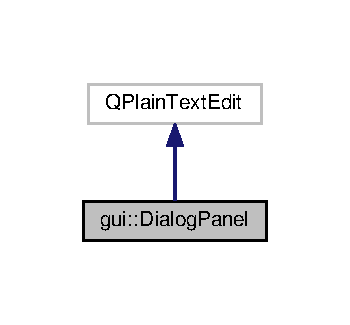
\includegraphics[width=168pt]{classgui_1_1DialogPanel__inherit__graph}
\end{center}
\end{figure}


Collaboration diagram for gui\+:\+:Dialog\+Panel\+:\nopagebreak
\begin{figure}[H]
\begin{center}
\leavevmode
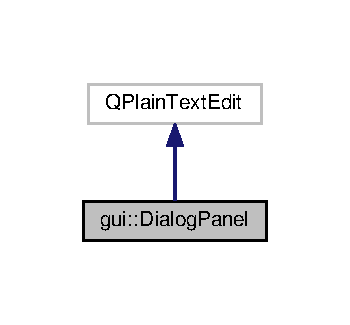
\includegraphics[width=168pt]{classgui_1_1DialogPanel__coll__graph}
\end{center}
\end{figure}
\subsection*{Public Member Functions}
\begin{DoxyCompactItemize}
\item 
\hyperlink{classgui_1_1DialogPanel_a38fc88cf71917935c2bd6275632ed019}{Dialog\+Panel} (Q\+Widget $\ast$parent=0)\hypertarget{classgui_1_1DialogPanel_a38fc88cf71917935c2bd6275632ed019}{}\label{classgui_1_1DialogPanel_a38fc88cf71917935c2bd6275632ed019}

\begin{DoxyCompactList}\small\item\em constructor \end{DoxyCompactList}\item 
\hyperlink{classgui_1_1DialogPanel_acfabd30363c9b93de4bb5f098a602ad7}{$\sim$\+Dialog\+Panel} ()\hypertarget{classgui_1_1DialogPanel_acfabd30363c9b93de4bb5f098a602ad7}{}\label{classgui_1_1DialogPanel_acfabd30363c9b93de4bb5f098a602ad7}

\begin{DoxyCompactList}\small\item\em destructor \end{DoxyCompactList}\item 
void \hyperlink{classgui_1_1DialogPanel_a584e9355ed1c9dff754b2682075365b8}{echo} (const Q\+String \&s)\hypertarget{classgui_1_1DialogPanel_a584e9355ed1c9dff754b2682075365b8}{}\label{classgui_1_1DialogPanel_a584e9355ed1c9dff754b2682075365b8}

\begin{DoxyCompactList}\small\item\em Write Q\+String s into the Q\+Plain\+Text\+Edit widget. \end{DoxyCompactList}\end{DoxyCompactItemize}
\subsection*{Protected Member Functions}
\begin{DoxyCompactItemize}
\item 
void {\bfseries mouse\+Press\+Event} (Q\+Mouse\+Event $\ast$e) Q\+\_\+\+D\+E\+C\+L\+\_\+\+O\+V\+E\+R\+R\+I\+DE\hypertarget{classgui_1_1DialogPanel_a1b9636870f3995c453e2bb9176940e88}{}\label{classgui_1_1DialogPanel_a1b9636870f3995c453e2bb9176940e88}

\end{DoxyCompactItemize}


The documentation for this class was generated from the following files\+:\begin{DoxyCompactItemize}
\item 
src/gui/widgets/\hyperlink{dialog__panel_8h}{dialog\+\_\+panel.\+h}\item 
src/gui/widgets/dialog\+\_\+panel.\+cc\end{DoxyCompactItemize}

\hypertarget{structprim_1_1SimJob_1_1elecDist}{}\section{prim\+:\+:Sim\+Job\+:\+:elec\+Dist Struct Reference}
\label{structprim_1_1SimJob_1_1elecDist}\index{prim\+::\+Sim\+Job\+::elec\+Dist@{prim\+::\+Sim\+Job\+::elec\+Dist}}


elec\+\_\+dists struct for showing where electrons are  




{\ttfamily \#include $<$sim\+\_\+job.\+h$>$}

\subsection*{Public Attributes}
\begin{DoxyCompactItemize}
\item 
Q\+String {\bfseries dist\+\_\+str}\hypertarget{structprim_1_1SimJob_1_1elecDist_af4b0d9de4752f19b6f01887d64ef4107}{}\label{structprim_1_1SimJob_1_1elecDist_af4b0d9de4752f19b6f01887d64ef4107}

\item 
Q\+List$<$ int $>$ {\bfseries dist\+\_\+ls}\hypertarget{structprim_1_1SimJob_1_1elecDist_a4f37103a0e94ef31622f9978a7c8765f}{}\label{structprim_1_1SimJob_1_1elecDist_a4f37103a0e94ef31622f9978a7c8765f}

\item 
float {\bfseries energy}\hypertarget{structprim_1_1SimJob_1_1elecDist_af735f97907807b1f3283183f5637f9aa}{}\label{structprim_1_1SimJob_1_1elecDist_af735f97907807b1f3283183f5637f9aa}

\end{DoxyCompactItemize}


\subsection{Detailed Description}
elec\+\_\+dists struct for showing where electrons are 

The documentation for this struct was generated from the following file\+:\begin{DoxyCompactItemize}
\item 
src/gui/widgets/primitives/\hyperlink{sim__job_8h}{sim\+\_\+job.\+h}\end{DoxyCompactItemize}

\hypertarget{classprim_1_1Electrode}{}\section{prim\+:\+:Electrode Class Reference}
\label{classprim_1_1Electrode}\index{prim\+::\+Electrode@{prim\+::\+Electrode}}


Inheritance diagram for prim\+:\+:Electrode\+:\nopagebreak
\begin{figure}[H]
\begin{center}
\leavevmode
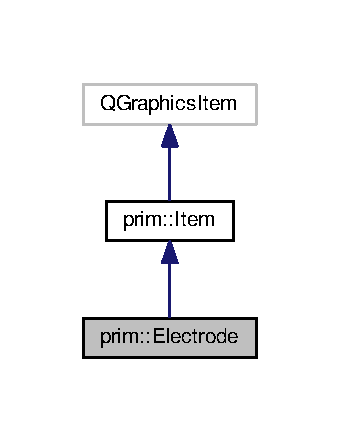
\includegraphics[width=163pt]{classprim_1_1Electrode__inherit__graph}
\end{center}
\end{figure}


Collaboration diagram for prim\+:\+:Electrode\+:\nopagebreak
\begin{figure}[H]
\begin{center}
\leavevmode
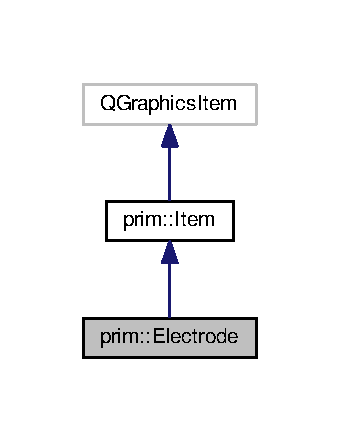
\includegraphics[width=163pt]{classprim_1_1Electrode__coll__graph}
\end{center}
\end{figure}
\subsection*{Public Types}
\begin{DoxyCompactItemize}
\item 
enum \hyperlink{classprim_1_1Electrode_a6b0ec865c0415eb2d43089c8c10ed389}{Electrode\+Type} \{ {\bfseries Clock}, 
{\bfseries Fix}
 \}\hypertarget{classprim_1_1Electrode_a6b0ec865c0415eb2d43089c8c10ed389}{}\label{classprim_1_1Electrode_a6b0ec865c0415eb2d43089c8c10ed389}
\begin{DoxyCompactList}\small\item\em Clock types will vary over time. Fix types are static. \end{DoxyCompactList}
\end{DoxyCompactItemize}
\subsection*{Public Member Functions}
\begin{DoxyCompactItemize}
\item 
\hyperlink{classprim_1_1Electrode_a40012efb5f084bd3badafbcd50cb51c2}{Electrode} (int lay\+\_\+id, Q\+PointF point1, Q\+PointF point2)\hypertarget{classprim_1_1Electrode_a40012efb5f084bd3badafbcd50cb51c2}{}\label{classprim_1_1Electrode_a40012efb5f084bd3badafbcd50cb51c2}

\begin{DoxyCompactList}\small\item\em constructor, creates an electrode given two points. \end{DoxyCompactList}\item 
\hyperlink{classprim_1_1Electrode_a85d5f70eb1a37b0170e3518343cc4d64}{Electrode} (Q\+Xml\+Stream\+Reader $\ast$ls, Q\+Graphics\+Scene $\ast$scene)\hypertarget{classprim_1_1Electrode_a85d5f70eb1a37b0170e3518343cc4d64}{}\label{classprim_1_1Electrode_a85d5f70eb1a37b0170e3518343cc4d64}

\begin{DoxyCompactList}\small\item\em constructor, creates an electrode from the design file. \end{DoxyCompactList}\item 
\hyperlink{classprim_1_1Electrode_a919a606690a1e381258d140c5f48015b}{$\sim$\+Electrode} ()\hypertarget{classprim_1_1Electrode_a919a606690a1e381258d140c5f48015b}{}\label{classprim_1_1Electrode_a919a606690a1e381258d140c5f48015b}

\begin{DoxyCompactList}\small\item\em destructor \end{DoxyCompactList}\item 
void {\bfseries init\+Electrode} (int lay\+\_\+id, Q\+PointF point1\+\_\+in, Q\+PointF point2\+\_\+in, double potential\+\_\+in=0, int electrode\+\_\+type\+\_\+in=0)\hypertarget{classprim_1_1Electrode_a15cdfde52ab38084a346e9191355cf49}{}\label{classprim_1_1Electrode_a15cdfde52ab38084a346e9191355cf49}

\item 
void \hyperlink{classprim_1_1Electrode_af5632f8ee7b20a9c82c2ffecad27cd7f}{set\+Potential} (double given\+Potential)\hypertarget{classprim_1_1Electrode_af5632f8ee7b20a9c82c2ffecad27cd7f}{}\label{classprim_1_1Electrode_af5632f8ee7b20a9c82c2ffecad27cd7f}

\begin{DoxyCompactList}\small\item\em sets the electrode potential to given\+Potential. \end{DoxyCompactList}\item 
double \hyperlink{classprim_1_1Electrode_a1cc37c6f2cca529cebf3769172adbd3c}{get\+Potential} (void) const \hypertarget{classprim_1_1Electrode_a1cc37c6f2cca529cebf3769172adbd3c}{}\label{classprim_1_1Electrode_a1cc37c6f2cca529cebf3769172adbd3c}

\begin{DoxyCompactList}\small\item\em gets the electrode potential to given\+Potential. \end{DoxyCompactList}\item 
Q\+PointF {\bfseries get\+Point1} (void)\hypertarget{classprim_1_1Electrode_ad04a8f9556a1826755eae2ce074e0b9a}{}\label{classprim_1_1Electrode_ad04a8f9556a1826755eae2ce074e0b9a}

\item 
Q\+PointF {\bfseries get\+Point2} (void)\hypertarget{classprim_1_1Electrode_a035953e2a9d0a9c677846dc403f73c3a}{}\label{classprim_1_1Electrode_a035953e2a9d0a9c677846dc403f73c3a}

\item 
Q\+PointF {\bfseries get\+Top\+Left} (void)\hypertarget{classprim_1_1Electrode_aed20c1872db9d76852c713462399bca6}{}\label{classprim_1_1Electrode_aed20c1872db9d76852c713462399bca6}

\item 
qreal {\bfseries get\+Top\+Depth} (void)\hypertarget{classprim_1_1Electrode_a2000e1e634b0cb469bbd0d5bf97c1977}{}\label{classprim_1_1Electrode_a2000e1e634b0cb469bbd0d5bf97c1977}

\item 
qreal {\bfseries get\+Width} (void)\hypertarget{classprim_1_1Electrode_a3bd6eba499c1e975d03ef3af51d6c4d1}{}\label{classprim_1_1Electrode_a3bd6eba499c1e975d03ef3af51d6c4d1}

\item 
qreal {\bfseries get\+Height} (void)\hypertarget{classprim_1_1Electrode_af38e81c23915d966223357fc4de3a08b}{}\label{classprim_1_1Electrode_af38e81c23915d966223357fc4de3a08b}

\item 
qreal {\bfseries get\+Depth} (void)\hypertarget{classprim_1_1Electrode_ade46d0bd594437e8342f788bd399873e}{}\label{classprim_1_1Electrode_ade46d0bd594437e8342f788bd399873e}

\item 
void \hyperlink{classprim_1_1Electrode_aa0036facf3e638e569235e2ee51e87c9}{update\+Points} (Q\+PointF)\hypertarget{classprim_1_1Electrode_aa0036facf3e638e569235e2ee51e87c9}{}\label{classprim_1_1Electrode_aa0036facf3e638e569235e2ee51e87c9}

\begin{DoxyCompactList}\small\item\em Updates the electrode with its new location. Call this after moving the electrode. \end{DoxyCompactList}\item 
Q\+RectF {\bfseries bounding\+Rect} () const Q\+\_\+\+D\+E\+C\+L\+\_\+\+O\+V\+E\+R\+R\+I\+DE\hypertarget{classprim_1_1Electrode_a39a58d3775880574d3f1f2d56cd3d9b3}{}\label{classprim_1_1Electrode_a39a58d3775880574d3f1f2d56cd3d9b3}

\item 
void {\bfseries paint} (Q\+Painter $\ast$, const Q\+Style\+Option\+Graphics\+Item $\ast$, Q\+Widget $\ast$) Q\+\_\+\+D\+E\+C\+L\+\_\+\+O\+V\+E\+R\+R\+I\+DE\hypertarget{classprim_1_1Electrode_afc04c7a7e27284d25519e26e073374f7}{}\label{classprim_1_1Electrode_afc04c7a7e27284d25519e26e073374f7}

\item 
\hyperlink{classprim_1_1Item}{Item} $\ast$ \hyperlink{classprim_1_1Electrode_a7a0a1265c745436bcd3ebe71a41751bc}{deep\+Copy} () const \hypertarget{classprim_1_1Electrode_a7a0a1265c745436bcd3ebe71a41751bc}{}\label{classprim_1_1Electrode_a7a0a1265c745436bcd3ebe71a41751bc}

\begin{DoxyCompactList}\small\item\em create a deep copy of the \hyperlink{classprim_1_1Item}{Item} for the clipboard. Deep-\/copied items should have no parent or scene and need only to have the information necessary to create a new copy somewhere in the scene \end{DoxyCompactList}\item 
virtual void {\bfseries save\+Items} (Q\+Xml\+Stream\+Writer $\ast$) const \hypertarget{classprim_1_1Electrode_a6c5afc878f2b8e25f22bef977da0340d}{}\label{classprim_1_1Electrode_a6c5afc878f2b8e25f22bef977da0340d}

\end{DoxyCompactItemize}
\subsection*{Public Attributes}
\begin{DoxyCompactItemize}
\item 
\hyperlink{classprim_1_1Electrode_a6b0ec865c0415eb2d43089c8c10ed389}{Electrode\+Type} {\bfseries electrode\+\_\+type}\hypertarget{classprim_1_1Electrode_a1e5555cb6418d80556719ae60e4191fc}{}\label{classprim_1_1Electrode_a1e5555cb6418d80556719ae60e4191fc}

\end{DoxyCompactItemize}
\subsection*{Protected Member Functions}
\begin{DoxyCompactItemize}
\item 
virtual void {\bfseries mouse\+Press\+Event} (Q\+Graphics\+Scene\+Mouse\+Event $\ast$e) Q\+\_\+\+D\+E\+C\+L\+\_\+\+O\+V\+E\+R\+R\+I\+DE\hypertarget{classprim_1_1Electrode_a935a6b74faadff87ba042fdb3ed66f6a}{}\label{classprim_1_1Electrode_a935a6b74faadff87ba042fdb3ed66f6a}

\item 
virtual void {\bfseries mouse\+Double\+Click\+Event} (Q\+Graphics\+Scene\+Mouse\+Event $\ast$e) Q\+\_\+\+D\+E\+C\+L\+\_\+\+O\+V\+E\+R\+R\+I\+DE\hypertarget{classprim_1_1Electrode_ad60d17ededd7096d18087432fdb68e9f}{}\label{classprim_1_1Electrode_ad60d17ededd7096d18087432fdb68e9f}

\end{DoxyCompactItemize}
\subsection*{Additional Inherited Members}


The documentation for this class was generated from the following files\+:\begin{DoxyCompactItemize}
\item 
src/gui/widgets/primitives/\hyperlink{electrode_8h}{electrode.\+h}\item 
src/gui/widgets/primitives/electrode.\+cc\end{DoxyCompactItemize}

\hypertarget{classprim_1_1Emitter}{}\section{prim\+:\+:Emitter Class Reference}
\label{classprim_1_1Emitter}\index{prim\+::\+Emitter@{prim\+::\+Emitter}}


Inheritance diagram for prim\+:\+:Emitter\+:\nopagebreak
\begin{figure}[H]
\begin{center}
\leavevmode
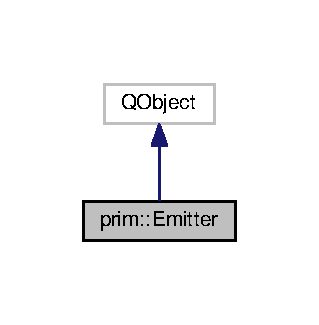
\includegraphics[width=153pt]{classprim_1_1Emitter__inherit__graph}
\end{center}
\end{figure}


Collaboration diagram for prim\+:\+:Emitter\+:\nopagebreak
\begin{figure}[H]
\begin{center}
\leavevmode
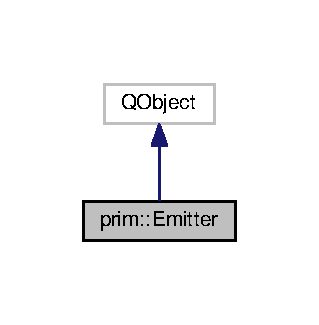
\includegraphics[width=153pt]{classprim_1_1Emitter__coll__graph}
\end{center}
\end{figure}
\subsection*{Signals}
\begin{DoxyCompactItemize}
\item 
void {\bfseries sig\+\_\+select\+Clicked} (\hyperlink{classprim_1_1Item}{Item} $\ast$)\hypertarget{classprim_1_1Emitter_a82a2a380009e179e7b9f7b04d7ffeab8}{}\label{classprim_1_1Emitter_a82a2a380009e179e7b9f7b04d7ffeab8}

\item 
void {\bfseries sig\+\_\+add\+Item\+To\+Scene} (\hyperlink{classprim_1_1Item}{Item} $\ast$)\hypertarget{classprim_1_1Emitter_a8f1dbfa8fd13fd1007c85492f1fc6e90}{}\label{classprim_1_1Emitter_a8f1dbfa8fd13fd1007c85492f1fc6e90}

\item 
void {\bfseries sig\+\_\+remove\+Item\+From\+Scene} (\hyperlink{classprim_1_1Item}{Item} $\ast$)\hypertarget{classprim_1_1Emitter_a4f5d3eb263a7821c97c705937f85f9f6}{}\label{classprim_1_1Emitter_a4f5d3eb263a7821c97c705937f85f9f6}

\end{DoxyCompactItemize}
\subsection*{Public Member Functions}
\begin{DoxyCompactItemize}
\item 
void \hyperlink{classprim_1_1Emitter_a2db5f282e69806d7cc527aa1008e5a51}{select\+Clicked} (\hyperlink{classprim_1_1Item}{Item} $\ast$)\hypertarget{classprim_1_1Emitter_a2db5f282e69806d7cc527aa1008e5a51}{}\label{classprim_1_1Emitter_a2db5f282e69806d7cc527aa1008e5a51}

\begin{DoxyCompactList}\small\item\em emit a signal indicating the given item has been clicked \end{DoxyCompactList}\item 
void \hyperlink{classprim_1_1Emitter_a9be15bb962c444c37cb539de62c1ffef}{add\+Item\+To\+Scene} (\hyperlink{classprim_1_1Item}{Item} $\ast$)\hypertarget{classprim_1_1Emitter_a9be15bb962c444c37cb539de62c1ffef}{}\label{classprim_1_1Emitter_a9be15bb962c444c37cb539de62c1ffef}

\begin{DoxyCompactList}\small\item\em emit a signal telling Design\+Panel to add item to scene \end{DoxyCompactList}\item 
void \hyperlink{classprim_1_1Emitter_a5fc17d7e621739edb04cd7d40e41ab40}{remove\+Item\+From\+Scene} (\hyperlink{classprim_1_1Item}{Item} $\ast$)\hypertarget{classprim_1_1Emitter_a5fc17d7e621739edb04cd7d40e41ab40}{}\label{classprim_1_1Emitter_a5fc17d7e621739edb04cd7d40e41ab40}

\begin{DoxyCompactList}\small\item\em emit a signal telling Design\+Panel to remove item from scene \end{DoxyCompactList}\end{DoxyCompactItemize}
\subsection*{Static Public Member Functions}
\begin{DoxyCompactItemize}
\item 
static \hyperlink{classprim_1_1Emitter}{Emitter} $\ast$ \hyperlink{classprim_1_1Emitter_a8a8b61c4476a094114c8dc51501e99f3}{instance} ()\hypertarget{classprim_1_1Emitter_a8a8b61c4476a094114c8dc51501e99f3}{}\label{classprim_1_1Emitter_a8a8b61c4476a094114c8dc51501e99f3}

\begin{DoxyCompactList}\small\item\em get or create static instance of \hyperlink{classprim_1_1Emitter}{Emitter} object \end{DoxyCompactList}\item 
static void \hyperlink{classprim_1_1Emitter_a3ac1e476e833c1249705f976f828a597}{clear} ()\hypertarget{classprim_1_1Emitter_a3ac1e476e833c1249705f976f828a597}{}\label{classprim_1_1Emitter_a3ac1e476e833c1249705f976f828a597}

\begin{DoxyCompactList}\small\item\em delete the static instance \end{DoxyCompactList}\end{DoxyCompactItemize}


The documentation for this class was generated from the following files\+:\begin{DoxyCompactItemize}
\item 
src/gui/widgets/primitives/\hyperlink{emitter_8h}{emitter.\+h}\item 
src/gui/widgets/primitives/emitter.\+cc\end{DoxyCompactItemize}

\hypertarget{structprim_1_1SimEngine_1_1ExpectedSimParam}{}\section{prim\+:\+:Sim\+Engine\+:\+:Expected\+Sim\+Param Struct Reference}
\label{structprim_1_1SimEngine_1_1ExpectedSimParam}\index{prim\+::\+Sim\+Engine\+::\+Expected\+Sim\+Param@{prim\+::\+Sim\+Engine\+::\+Expected\+Sim\+Param}}


types of sim params expected for this engine  




{\ttfamily \#include $<$sim\+\_\+engine.\+h$>$}

\subsection*{Public Member Functions}
\begin{DoxyCompactItemize}
\item 
{\bfseries Expected\+Sim\+Param} (const Q\+String \&param\+\_\+nm, const Q\+String \&g\+\_\+obj\+\_\+nm, const Q\+String \&g\+\_\+obj\+\_\+type, const Q\+String \&g\+\_\+def\+\_\+txt=Q\+String())\hypertarget{structprim_1_1SimEngine_1_1ExpectedSimParam_a89d4509bd7f5abd86a6bf5b799c7a1b2}{}\label{structprim_1_1SimEngine_1_1ExpectedSimParam_a89d4509bd7f5abd86a6bf5b799c7a1b2}

\end{DoxyCompactItemize}
\subsection*{Public Attributes}
\begin{DoxyCompactItemize}
\item 
Q\+String {\bfseries name}\hypertarget{structprim_1_1SimEngine_1_1ExpectedSimParam_af0bf0e1278ccb3f1eb3601c48fc82a6d}{}\label{structprim_1_1SimEngine_1_1ExpectedSimParam_af0bf0e1278ccb3f1eb3601c48fc82a6d}

\item 
Q\+String {\bfseries gui\+\_\+object\+\_\+name}\hypertarget{structprim_1_1SimEngine_1_1ExpectedSimParam_a431b9baebb27844d4c7ed2c71f61c294}{}\label{structprim_1_1SimEngine_1_1ExpectedSimParam_a431b9baebb27844d4c7ed2c71f61c294}

\item 
Q\+String {\bfseries gui\+\_\+object\+\_\+type}\hypertarget{structprim_1_1SimEngine_1_1ExpectedSimParam_a50d14d3bdb5829ff49d0beef7ea977c1}{}\label{structprim_1_1SimEngine_1_1ExpectedSimParam_a50d14d3bdb5829ff49d0beef7ea977c1}

\item 
Q\+String {\bfseries gui\+\_\+default\+\_\+text}\hypertarget{structprim_1_1SimEngine_1_1ExpectedSimParam_ae7e0551ee8433d287587bbc71a157595}{}\label{structprim_1_1SimEngine_1_1ExpectedSimParam_ae7e0551ee8433d287587bbc71a157595}

\end{DoxyCompactItemize}


\subsection{Detailed Description}
types of sim params expected for this engine 

The documentation for this struct was generated from the following file\+:\begin{DoxyCompactItemize}
\item 
src/gui/widgets/primitives/sim\+\_\+engine.\+h\end{DoxyCompactItemize}

\hypertarget{classgui_1_1DesignPanel_1_1FormAggregate}{}\section{gui\+:\+:Design\+Panel\+:\+:Form\+Aggregate Class Reference}
\label{classgui_1_1DesignPanel_1_1FormAggregate}\index{gui\+::\+Design\+Panel\+::\+Form\+Aggregate@{gui\+::\+Design\+Panel\+::\+Form\+Aggregate}}


Inheritance diagram for gui\+:\+:Design\+Panel\+:\+:Form\+Aggregate\+:\nopagebreak
\begin{figure}[H]
\begin{center}
\leavevmode
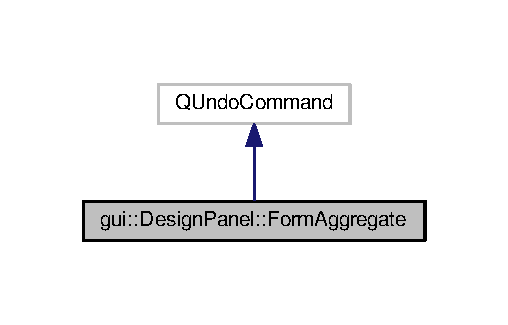
\includegraphics[width=244pt]{classgui_1_1DesignPanel_1_1FormAggregate__inherit__graph}
\end{center}
\end{figure}


Collaboration diagram for gui\+:\+:Design\+Panel\+:\+:Form\+Aggregate\+:\nopagebreak
\begin{figure}[H]
\begin{center}
\leavevmode
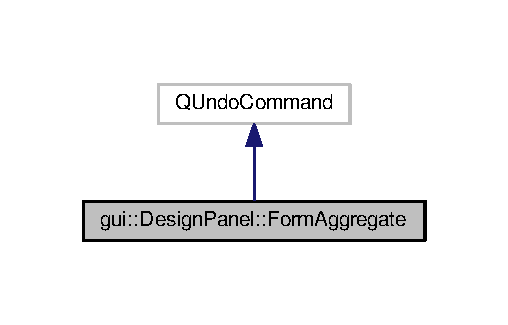
\includegraphics[width=244pt]{classgui_1_1DesignPanel_1_1FormAggregate__coll__graph}
\end{center}
\end{figure}
\subsection*{Public Member Functions}
\begin{DoxyCompactItemize}
\item 
{\bfseries Form\+Aggregate} (Q\+List$<$ \hyperlink{classprim_1_1Item}{prim\+::\+Item} $\ast$ $>$ \&items, \hyperlink{classgui_1_1DesignPanel}{Design\+Panel} $\ast$dp, Q\+Undo\+Command $\ast$parent=0)\hypertarget{classgui_1_1DesignPanel_1_1FormAggregate_a62abcd9d0c89992639623cf076639771}{}\label{classgui_1_1DesignPanel_1_1FormAggregate_a62abcd9d0c89992639623cf076639771}

\item 
{\bfseries Form\+Aggregate} (\hyperlink{classprim_1_1Aggregate}{prim\+::\+Aggregate} $\ast$agg, int offset, \hyperlink{classgui_1_1DesignPanel}{Design\+Panel} $\ast$dp, Q\+Undo\+Command $\ast$parent=0)\hypertarget{classgui_1_1DesignPanel_1_1FormAggregate_a191472adbd2388b6c5ebadcbda122a07}{}\label{classgui_1_1DesignPanel_1_1FormAggregate_a191472adbd2388b6c5ebadcbda122a07}

\item 
virtual void {\bfseries undo} ()\hypertarget{classgui_1_1DesignPanel_1_1FormAggregate_abe4938b2bbcb5a963d20142b643df287}{}\label{classgui_1_1DesignPanel_1_1FormAggregate_abe4938b2bbcb5a963d20142b643df287}

\item 
virtual void {\bfseries redo} ()\hypertarget{classgui_1_1DesignPanel_1_1FormAggregate_a399210ee2d517994871d6d5f91fcf364}{}\label{classgui_1_1DesignPanel_1_1FormAggregate_a399210ee2d517994871d6d5f91fcf364}

\end{DoxyCompactItemize}


The documentation for this class was generated from the following files\+:\begin{DoxyCompactItemize}
\item 
src/gui/widgets/\hyperlink{design__panel_8h}{design\+\_\+panel.\+h}\item 
src/gui/widgets/design\+\_\+panel.\+cc\end{DoxyCompactItemize}

\hypertarget{classprim_1_1Ghost}{}\section{prim\+:\+:Ghost Class Reference}
\label{classprim_1_1Ghost}\index{prim\+::\+Ghost@{prim\+::\+Ghost}}


collection of \hyperlink{classprim_1_1GhostDot}{Ghost\+Dot} and \hyperlink{classprim_1_1GhostBox}{Ghost\+Box} objects for moving Items or copy/paste, singleton  




{\ttfamily \#include $<$ghost.\+h$>$}



Inheritance diagram for prim\+:\+:Ghost\+:\nopagebreak
\begin{figure}[H]
\begin{center}
\leavevmode
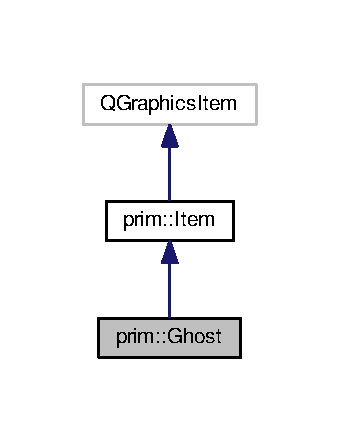
\includegraphics[width=163pt]{classprim_1_1Ghost__inherit__graph}
\end{center}
\end{figure}


Collaboration diagram for prim\+:\+:Ghost\+:\nopagebreak
\begin{figure}[H]
\begin{center}
\leavevmode
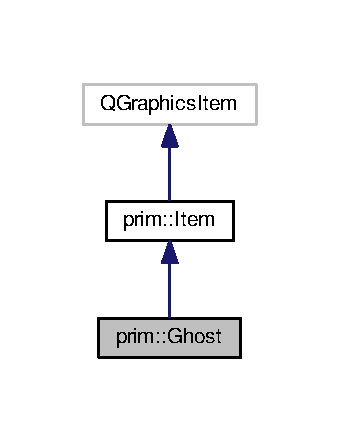
\includegraphics[width=163pt]{classprim_1_1Ghost__coll__graph}
\end{center}
\end{figure}
\subsection*{Public Member Functions}
\begin{DoxyCompactItemize}
\item 
\hyperlink{classprim_1_1Ghost_ad2c6d5babda20b32619b8801c1f8d94a}{$\sim$\+Ghost} ()\hypertarget{classprim_1_1Ghost_ad2c6d5babda20b32619b8801c1f8d94a}{}\label{classprim_1_1Ghost_ad2c6d5babda20b32619b8801c1f8d94a}

\begin{DoxyCompactList}\small\item\em destructor, potentially useful later \end{DoxyCompactList}\item 
void \hyperlink{classprim_1_1Ghost_a4218723c157248b5d7336c7381110316}{clean\+Ghost} ()\hypertarget{classprim_1_1Ghost_a4218723c157248b5d7336c7381110316}{}\label{classprim_1_1Ghost_a4218723c157248b5d7336c7381110316}

\begin{DoxyCompactList}\small\item\em reset \hyperlink{classprim_1_1Ghost}{Ghost} to its empty state \end{DoxyCompactList}\item 
void \hyperlink{classprim_1_1Ghost_ad8b7351f2d73c9793f39571c79e3abcf}{set\+Scene} (Q\+Graphics\+Scene $\ast$sc)\hypertarget{classprim_1_1Ghost_ad8b7351f2d73c9793f39571c79e3abcf}{}\label{classprim_1_1Ghost_ad8b7351f2d73c9793f39571c79e3abcf}

\begin{DoxyCompactList}\small\item\em Add the current \hyperlink{classprim_1_1Ghost}{Ghost} to sc. \end{DoxyCompactList}\item 
void \hyperlink{classprim_1_1Ghost_a61f8b226d0feb571f0cba1d27029c231}{prepare} (const Q\+List$<$ \hyperlink{classprim_1_1Item}{prim\+::\+Item} $\ast$ $>$ \&items, Q\+PointF scene\+\_\+pos=Q\+PointF())\hypertarget{classprim_1_1Ghost_a61f8b226d0feb571f0cba1d27029c231}{}\label{classprim_1_1Ghost_a61f8b226d0feb571f0cba1d27029c231}

\begin{DoxyCompactList}\small\item\em create a ghost image from a list of \hyperlink{classprim_1_1Item}{Item} objects if moving, scene\+\_\+pos gives the current mouse location \end{DoxyCompactList}\item 
void \hyperlink{classprim_1_1Ghost_a8e92d9b86e2f9ebcdf2849de63fb87f9}{prepare} (\hyperlink{classprim_1_1Item}{Item} $\ast$item, Q\+PointF scene\+\_\+pos=Q\+PointF())\hypertarget{classprim_1_1Ghost_a8e92d9b86e2f9ebcdf2849de63fb87f9}{}\label{classprim_1_1Ghost_a8e92d9b86e2f9ebcdf2849de63fb87f9}

\begin{DoxyCompactList}\small\item\em create a ghost image from a single \hyperlink{classprim_1_1Item}{Item} if moving, scene\+\_\+pos gives the current mouse location \end{DoxyCompactList}\item 
void \hyperlink{classprim_1_1Ghost_a1f51f724ed50b9a152ce590e5fc865bd}{move\+To} (Q\+PointF pos)\hypertarget{classprim_1_1Ghost_a1f51f724ed50b9a152ce590e5fc865bd}{}\label{classprim_1_1Ghost_a1f51f724ed50b9a152ce590e5fc865bd}

\begin{DoxyCompactList}\small\item\em move center of \hyperlink{classprim_1_1Ghost}{Ghost} to the given position \end{DoxyCompactList}\item 
Q\+List$<$ \hyperlink{classprim_1_1Item}{prim\+::\+Item} $\ast$ $>$ \& \hyperlink{classprim_1_1Ghost_ac765bda81aa6c2e1d484cf11b7a53b40}{get\+Sources} ()\hypertarget{classprim_1_1Ghost_ac765bda81aa6c2e1d484cf11b7a53b40}{}\label{classprim_1_1Ghost_ac765bda81aa6c2e1d484cf11b7a53b40}

\begin{DoxyCompactList}\small\item\em get the items associated with the Ghost\+Dots \end{DoxyCompactList}\item 
Q\+List$<$ \hyperlink{classprim_1_1GhostDot}{prim\+::\+Ghost\+Dot} $\ast$ $>$ \hyperlink{classprim_1_1Ghost_a6046201ee3e54a1ff5f8ce06e4076034}{get\+Dots} ()\hypertarget{classprim_1_1Ghost_a6046201ee3e54a1ff5f8ce06e4076034}{}\label{classprim_1_1Ghost_a6046201ee3e54a1ff5f8ce06e4076034}

\begin{DoxyCompactList}\small\item\em get the Ghost\+Dots \end{DoxyCompactList}\item 
Q\+List$<$ \hyperlink{classprim_1_1Item}{prim\+::\+Item} $\ast$ $>$ \& \hyperlink{classprim_1_1Ghost_a8588e78ab2471a42cec11ed206f12ba8}{get\+Box\+Sources} ()\hypertarget{classprim_1_1Ghost_a8588e78ab2471a42cec11ed206f12ba8}{}\label{classprim_1_1Ghost_a8588e78ab2471a42cec11ed206f12ba8}

\begin{DoxyCompactList}\small\item\em get the items associated with the Ghost\+Boxes \end{DoxyCompactList}\item 
Q\+List$<$ \hyperlink{classprim_1_1GhostBox}{prim\+::\+Ghost\+Box} $\ast$ $>$ \hyperlink{classprim_1_1Ghost_a3ab6cb77d198a866c036253278778f49}{get\+Boxes} ()\hypertarget{classprim_1_1Ghost_a3ab6cb77d198a866c036253278778f49}{}\label{classprim_1_1Ghost_a3ab6cb77d198a866c036253278778f49}

\begin{DoxyCompactList}\small\item\em get the Ghost\+Boxes \end{DoxyCompactList}\item 
Q\+List$<$ \hyperlink{classprim_1_1Item}{prim\+::\+Item} $\ast$ $>$ \hyperlink{classprim_1_1Ghost_a920aa6435950563ae70262dcd69df7d4}{get\+Top\+Items} () const \hypertarget{classprim_1_1Ghost_a920aa6435950563ae70262dcd69df7d4}{}\label{classprim_1_1Ghost_a920aa6435950563ae70262dcd69df7d4}

\begin{DoxyCompactList}\small\item\em get a list of the highest level Items associated with the sources \end{DoxyCompactList}\item 
\hyperlink{structprim_1_1AggNode}{prim\+::\+Agg\+Node} \& \hyperlink{classprim_1_1Ghost_af75764943e4245ef8c4825bdbfadec7e}{get\+Top\+Indices} ()\hypertarget{classprim_1_1Ghost_af75764943e4245ef8c4825bdbfadec7e}{}\label{classprim_1_1Ghost_af75764943e4245ef8c4825bdbfadec7e}

\begin{DoxyCompactList}\small\item\em get a nested list of the items included in each high level item, must free Index\+List pointer after use \end{DoxyCompactList}\item 
Q\+List$<$ \hyperlink{classprim_1_1LatticeDot}{prim\+::\+Lattice\+Dot} $\ast$ $>$ \hyperlink{classprim_1_1Ghost_a641a82fd79a022ade58f9a3f392647e2}{get\+Lattice} (const Q\+PointF \&offset=Q\+PointF()) const \hypertarget{classprim_1_1Ghost_a641a82fd79a022ade58f9a3f392647e2}{}\label{classprim_1_1Ghost_a641a82fd79a022ade58f9a3f392647e2}

\begin{DoxyCompactList}\small\item\em get a list corresponding to the \hyperlink{classprim_1_1LatticeDot}{Lattice\+Dot} associated with each \hyperlink{classprim_1_1GhostDot}{Ghost\+Dot}. If the \hyperlink{classprim_1_1Item}{Item} associated with the \hyperlink{classprim_1_1GhostDot}{Ghost\+Dot} is not a dangling bond the list will contain a 0. \end{DoxyCompactList}\item 
\hyperlink{classprim_1_1LatticeDot}{prim\+::\+Lattice\+Dot} $\ast$ \hyperlink{classprim_1_1Ghost_a3d5a8778efd339414b0d37faba25c1dd}{get\+Lattice\+Dot} (\hyperlink{classprim_1_1DBDot}{prim\+::\+D\+B\+Dot} $\ast$db)\hypertarget{classprim_1_1Ghost_a3d5a8778efd339414b0d37faba25c1dd}{}\label{classprim_1_1Ghost_a3d5a8778efd339414b0d37faba25c1dd}

\begin{DoxyCompactList}\small\item\em attempt to get the lattice dot under the \hyperlink{classprim_1_1GhostDot}{Ghost\+Dot} correponding to the given \hyperlink{classprim_1_1DBDot}{D\+B\+Dot} item. \end{DoxyCompactList}\item 
\hyperlink{classprim_1_1GhostDot}{prim\+::\+Ghost\+Dot} $\ast$ \hyperlink{classprim_1_1Ghost_a2558b908740d3f990cc7fec51a058802}{snap\+Anchor} ()\hypertarget{classprim_1_1Ghost_a2558b908740d3f990cc7fec51a058802}{}\label{classprim_1_1Ghost_a2558b908740d3f990cc7fec51a058802}

\begin{DoxyCompactList}\small\item\em get the \hyperlink{classprim_1_1GhostDot}{Ghost\+Dot} nearest to the center of the \hyperlink{classprim_1_1Ghost}{Ghost}. If db is set, will return the neatest dangling bond \hyperlink{classprim_1_1GhostDot}{Ghost\+Dot} if any exists else 0. \end{DoxyCompactList}\item 
Q\+PointF \hyperlink{classprim_1_1Ghost_a070edb8e12dcbca0004419d84a1d6352}{free\+Anchor} (Q\+PointF scene\+\_\+pos)\hypertarget{classprim_1_1Ghost_a070edb8e12dcbca0004419d84a1d6352}{}\label{classprim_1_1Ghost_a070edb8e12dcbca0004419d84a1d6352}

\begin{DoxyCompactList}\small\item\em location of the anchor dot if the \hyperlink{classprim_1_1Ghost}{Ghost} were centered at the given scene position. \end{DoxyCompactList}\item 
Q\+Color $\ast$ \hyperlink{classprim_1_1Ghost_a5beebb67cf4a0b3f6bfc72af3e13055f}{get\+Col} ()\hypertarget{classprim_1_1Ghost_a5beebb67cf4a0b3f6bfc72af3e13055f}{}\label{classprim_1_1Ghost_a5beebb67cf4a0b3f6bfc72af3e13055f}

\begin{DoxyCompactList}\small\item\em getter for ghost color \end{DoxyCompactList}\item 
void \hyperlink{classprim_1_1Ghost_add66c0767f3e9251e3532c07f7357923}{set\+Col} (Q\+Color \&color)\hypertarget{classprim_1_1Ghost_add66c0767f3e9251e3532c07f7357923}{}\label{classprim_1_1Ghost_add66c0767f3e9251e3532c07f7357923}

\begin{DoxyCompactList}\small\item\em setter for ghost color \end{DoxyCompactList}\item 
void \hyperlink{classprim_1_1Ghost_a9f7ed79e6ea56dacad0f2c4a0f6a503d}{set\+Valid} (bool val)\hypertarget{classprim_1_1Ghost_a9f7ed79e6ea56dacad0f2c4a0f6a503d}{}\label{classprim_1_1Ghost_a9f7ed79e6ea56dacad0f2c4a0f6a503d}

\begin{DoxyCompactList}\small\item\em manual set for the validity of the current position \end{DoxyCompactList}\item 
bool \hyperlink{classprim_1_1Ghost_a353ab6dfe05cfff99aebab59207cb95d}{check\+Valid} (const Q\+PointF \&offset=Q\+PointF())\hypertarget{classprim_1_1Ghost_a353ab6dfe05cfff99aebab59207cb95d}{}\label{classprim_1_1Ghost_a353ab6dfe05cfff99aebab59207cb95d}

\begin{DoxyCompactList}\small\item\em check if the current position is valid. \end{DoxyCompactList}\item 
Q\+PointF \hyperlink{classprim_1_1Ghost_aae476432c09d4c3b3a8c8dcdb8a94c94}{move\+Offset} () const \hypertarget{classprim_1_1Ghost_aae476432c09d4c3b3a8c8dcdb8a94c94}{}\label{classprim_1_1Ghost_aae476432c09d4c3b3a8c8dcdb8a94c94}

\begin{DoxyCompactList}\small\item\em change in position between the first source and \hyperlink{classprim_1_1GhostDot}{Ghost\+Dot}, for moving Items \end{DoxyCompactList}\item 
Q\+RectF {\bfseries bounding\+Rect} () const Q\+\_\+\+D\+E\+C\+L\+\_\+\+O\+V\+E\+R\+R\+I\+DE\hypertarget{classprim_1_1Ghost_a67cf6c0546c09e90f86107f8c9b6c548}{}\label{classprim_1_1Ghost_a67cf6c0546c09e90f86107f8c9b6c548}

\item 
void {\bfseries paint} (Q\+Painter $\ast$painter, const Q\+Style\+Option\+Graphics\+Item $\ast$, Q\+Widget $\ast$) Q\+\_\+\+D\+E\+C\+L\+\_\+\+O\+V\+E\+R\+R\+I\+DE\hypertarget{classprim_1_1Ghost_ae9a5e4b678c702be051a96060e80082c}{}\label{classprim_1_1Ghost_ae9a5e4b678c702be051a96060e80082c}

\item 
\hyperlink{classprim_1_1Item}{prim\+::\+Item} $\ast$ \hyperlink{classprim_1_1Ghost_a93ee73c97062828642eafdd64d6211de}{deep\+Copy} () const \hypertarget{classprim_1_1Ghost_a93ee73c97062828642eafdd64d6211de}{}\label{classprim_1_1Ghost_a93ee73c97062828642eafdd64d6211de}

\begin{DoxyCompactList}\small\item\em create a deep copy of the \hyperlink{classprim_1_1Item}{Item} for the clipboard. Deep-\/copied items should have no parent or scene and need only to have the information necessary to create a new copy somewhere in the scene \end{DoxyCompactList}\item 
void {\bfseries echo\+Top\+Indices} ()\hypertarget{classprim_1_1Ghost_a9df8e28afe11ef1355672ba2c834c267}{}\label{classprim_1_1Ghost_a9df8e28afe11ef1355672ba2c834c267}

\item 
void {\bfseries echo\+Node} (Q\+String \&s, \hyperlink{structprim_1_1AggNode}{Agg\+Node} $\ast$node)\hypertarget{classprim_1_1Ghost_ac6766dd582591462577331a9b93b60ea}{}\label{classprim_1_1Ghost_ac6766dd582591462577331a9b93b60ea}

\end{DoxyCompactItemize}
\subsection*{Static Public Member Functions}
\begin{DoxyCompactItemize}
\item 
static \hyperlink{classprim_1_1Ghost}{Ghost} $\ast$ \hyperlink{classprim_1_1Ghost_a16931bddd932d534b0926826d20e1e90}{instance} ()\hypertarget{classprim_1_1Ghost_a16931bddd932d534b0926826d20e1e90}{}\label{classprim_1_1Ghost_a16931bddd932d534b0926826d20e1e90}

\begin{DoxyCompactList}\small\item\em get or create the static \hyperlink{classprim_1_1Ghost}{Ghost} instance \end{DoxyCompactList}\end{DoxyCompactItemize}
\subsection*{Public Attributes}
\begin{DoxyCompactItemize}
\item 
Q\+Hash$<$ \hyperlink{classprim_1_1LatticeDot}{prim\+::\+Lattice\+Dot} $\ast$, bool $>$ \hyperlink{classprim_1_1Ghost_abdb2bd655baa8cb186477355ff1d7a57}{valid\+\_\+hash}\hypertarget{classprim_1_1Ghost_abdb2bd655baa8cb186477355ff1d7a57}{}\label{classprim_1_1Ghost_abdb2bd655baa8cb186477355ff1d7a57}

\begin{DoxyCompactList}\small\item\em hash table for valid snap points \end{DoxyCompactList}\end{DoxyCompactItemize}
\subsection*{Additional Inherited Members}


\subsection{Detailed Description}
collection of \hyperlink{classprim_1_1GhostDot}{Ghost\+Dot} and \hyperlink{classprim_1_1GhostBox}{Ghost\+Box} objects for moving Items or copy/paste, singleton 

The documentation for this class was generated from the following files\+:\begin{DoxyCompactItemize}
\item 
src/gui/widgets/primitives/\hyperlink{ghost_8h}{ghost.\+h}\item 
src/gui/widgets/primitives/ghost.\+cc\end{DoxyCompactItemize}

\hypertarget{classprim_1_1GhostBox}{}\section{prim\+:\+:Ghost\+Box Class Reference}
\label{classprim_1_1GhostBox}\index{prim\+::\+Ghost\+Box@{prim\+::\+Ghost\+Box}}


The ghost associated with Electrodes. Used during move and previews.  




{\ttfamily \#include $<$ghost.\+h$>$}



Inheritance diagram for prim\+:\+:Ghost\+Box\+:\nopagebreak
\begin{figure}[H]
\begin{center}
\leavevmode
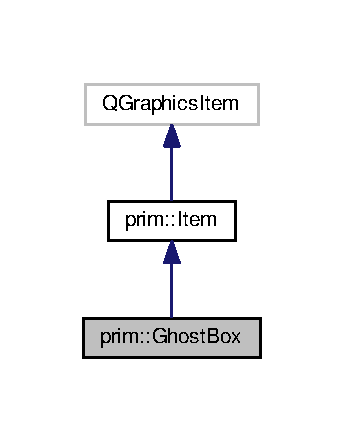
\includegraphics[width=165pt]{classprim_1_1GhostBox__inherit__graph}
\end{center}
\end{figure}


Collaboration diagram for prim\+:\+:Ghost\+Box\+:\nopagebreak
\begin{figure}[H]
\begin{center}
\leavevmode
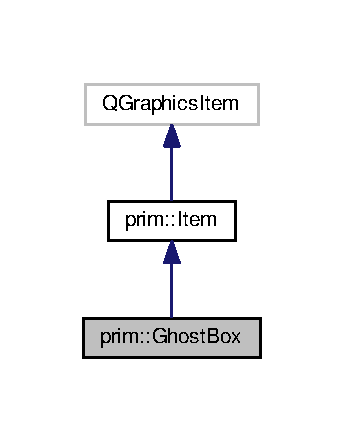
\includegraphics[width=165pt]{classprim_1_1GhostBox__coll__graph}
\end{center}
\end{figure}
\subsection*{Public Member Functions}
\begin{DoxyCompactItemize}
\item 
\hyperlink{classprim_1_1GhostBox_a53ca4c643d84fd75c8b5469a8d5789d1}{Ghost\+Box} (\hyperlink{classprim_1_1Item}{Item} $\ast$item, \hyperlink{classprim_1_1Item}{Item} $\ast$parent)\hypertarget{classprim_1_1GhostBox_a53ca4c643d84fd75c8b5469a8d5789d1}{}\label{classprim_1_1GhostBox_a53ca4c643d84fd75c8b5469a8d5789d1}

\begin{DoxyCompactList}\small\item\em constructor \end{DoxyCompactList}\item 
\hyperlink{classprim_1_1GhostBox_aa1b26dcd2637e429bd9f0ae2b2947930}{$\sim$\+Ghost\+Box} ()\hypertarget{classprim_1_1GhostBox_aa1b26dcd2637e429bd9f0ae2b2947930}{}\label{classprim_1_1GhostBox_aa1b26dcd2637e429bd9f0ae2b2947930}

\begin{DoxyCompactList}\small\item\em destructor \end{DoxyCompactList}\item 
Q\+RectF {\bfseries bounding\+Rect} () const Q\+\_\+\+D\+E\+C\+L\+\_\+\+O\+V\+E\+R\+R\+I\+DE\hypertarget{classprim_1_1GhostBox_a63bdb5fc445b3b7887d4eb985046ab4a}{}\label{classprim_1_1GhostBox_a63bdb5fc445b3b7887d4eb985046ab4a}

\item 
void {\bfseries paint} (Q\+Painter $\ast$painter, const Q\+Style\+Option\+Graphics\+Item $\ast$, Q\+Widget $\ast$) Q\+\_\+\+D\+E\+C\+L\+\_\+\+O\+V\+E\+R\+R\+I\+DE\hypertarget{classprim_1_1GhostBox_a0dd5d2a098f9d2f691e69fb4f6ca70f4}{}\label{classprim_1_1GhostBox_a0dd5d2a098f9d2f691e69fb4f6ca70f4}

\item 
\hyperlink{classprim_1_1Item}{Item} $\ast$ \hyperlink{classprim_1_1GhostBox_a6395c270d96456bb625ba7e5f5173478}{deep\+Copy} () const \hypertarget{classprim_1_1GhostBox_a6395c270d96456bb625ba7e5f5173478}{}\label{classprim_1_1GhostBox_a6395c270d96456bb625ba7e5f5173478}

\begin{DoxyCompactList}\small\item\em create a deep copy of the \hyperlink{classprim_1_1Item}{Item} for the clipboard. Deep-\/copied items should have no parent or scene and need only to have the information necessary to create a new copy somewhere in the scene \end{DoxyCompactList}\end{DoxyCompactItemize}
\subsection*{Additional Inherited Members}


\subsection{Detailed Description}
The ghost associated with Electrodes. Used during move and previews. 

The documentation for this class was generated from the following files\+:\begin{DoxyCompactItemize}
\item 
src/gui/widgets/primitives/\hyperlink{ghost_8h}{ghost.\+h}\item 
src/gui/widgets/primitives/ghost.\+cc\end{DoxyCompactItemize}

\hypertarget{classprim_1_1GhostDot}{}\section{prim\+:\+:Ghost\+Dot Class Reference}
\label{classprim_1_1GhostDot}\index{prim\+::\+Ghost\+Dot@{prim\+::\+Ghost\+Dot}}


The ghost associated with D\+B\+Dots and Lattice\+Dots. Used during move and previews.  




{\ttfamily \#include $<$ghost.\+h$>$}



Inheritance diagram for prim\+:\+:Ghost\+Dot\+:\nopagebreak
\begin{figure}[H]
\begin{center}
\leavevmode
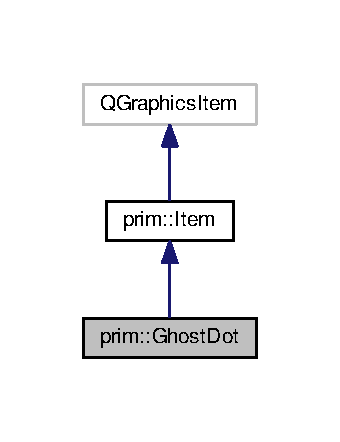
\includegraphics[width=163pt]{classprim_1_1GhostDot__inherit__graph}
\end{center}
\end{figure}


Collaboration diagram for prim\+:\+:Ghost\+Dot\+:\nopagebreak
\begin{figure}[H]
\begin{center}
\leavevmode
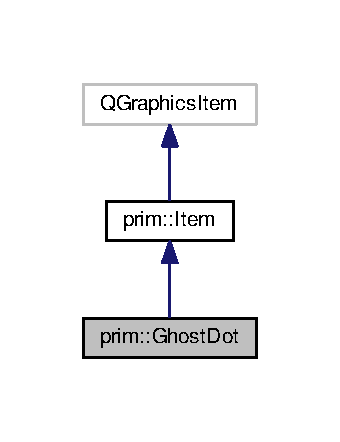
\includegraphics[width=163pt]{classprim_1_1GhostDot__coll__graph}
\end{center}
\end{figure}
\subsection*{Public Member Functions}
\begin{DoxyCompactItemize}
\item 
\hyperlink{classprim_1_1GhostDot_a39eceb1dc7b43a4b655850c6e951d18c}{Ghost\+Dot} (\hyperlink{classprim_1_1Item}{Item} $\ast$item, \hyperlink{classprim_1_1Item}{Item} $\ast$parent, Q\+Color $\ast$pcol)\hypertarget{classprim_1_1GhostDot_a39eceb1dc7b43a4b655850c6e951d18c}{}\label{classprim_1_1GhostDot_a39eceb1dc7b43a4b655850c6e951d18c}

\begin{DoxyCompactList}\small\item\em constructor \end{DoxyCompactList}\item 
\hyperlink{classprim_1_1GhostDot_adcf2798a87c26860e86e33b68569bcdb}{$\sim$\+Ghost\+Dot} ()\hypertarget{classprim_1_1GhostDot_adcf2798a87c26860e86e33b68569bcdb}{}\label{classprim_1_1GhostDot_adcf2798a87c26860e86e33b68569bcdb}

\begin{DoxyCompactList}\small\item\em destructor \end{DoxyCompactList}\item 
Q\+RectF {\bfseries bounding\+Rect} () const Q\+\_\+\+D\+E\+C\+L\+\_\+\+O\+V\+E\+R\+R\+I\+DE\hypertarget{classprim_1_1GhostDot_a5844a39b3e3d88d0e623f9fe1ceeb9b2}{}\label{classprim_1_1GhostDot_a5844a39b3e3d88d0e623f9fe1ceeb9b2}

\item 
void {\bfseries paint} (Q\+Painter $\ast$painter, const Q\+Style\+Option\+Graphics\+Item $\ast$, Q\+Widget $\ast$) Q\+\_\+\+D\+E\+C\+L\+\_\+\+O\+V\+E\+R\+R\+I\+DE\hypertarget{classprim_1_1GhostDot_a1dd50ebda0ec10345f11e57f3bd32e8a}{}\label{classprim_1_1GhostDot_a1dd50ebda0ec10345f11e57f3bd32e8a}

\item 
\hyperlink{classprim_1_1Item}{Item} $\ast$ \hyperlink{classprim_1_1GhostDot_a5c4aca3ca44cce6ace1f649b7b534d58}{deep\+Copy} () const \hypertarget{classprim_1_1GhostDot_a5c4aca3ca44cce6ace1f649b7b534d58}{}\label{classprim_1_1GhostDot_a5c4aca3ca44cce6ace1f649b7b534d58}

\begin{DoxyCompactList}\small\item\em create a deep copy of the \hyperlink{classprim_1_1Item}{Item} for the clipboard. Deep-\/copied items should have no parent or scene and need only to have the information necessary to create a new copy somewhere in the scene \end{DoxyCompactList}\end{DoxyCompactItemize}
\subsection*{Additional Inherited Members}


\subsection{Detailed Description}
The ghost associated with D\+B\+Dots and Lattice\+Dots. Used during move and previews. 

The documentation for this class was generated from the following files\+:\begin{DoxyCompactItemize}
\item 
src/gui/widgets/primitives/\hyperlink{ghost_8h}{ghost.\+h}\item 
src/gui/widgets/primitives/ghost.\+cc\end{DoxyCompactItemize}

\hypertarget{classsettings_1_1GUISettings}{}\section{settings\+:\+:G\+U\+I\+Settings Class Reference}
\label{classsettings_1_1GUISettings}\index{settings\+::\+G\+U\+I\+Settings@{settings\+::\+G\+U\+I\+Settings}}


Inheritance diagram for settings\+:\+:G\+U\+I\+Settings\+:\nopagebreak
\begin{figure}[H]
\begin{center}
\leavevmode
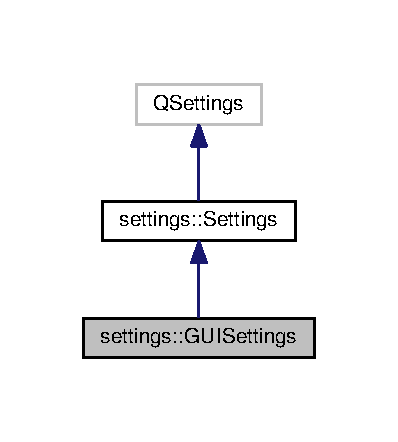
\includegraphics[width=191pt]{classsettings_1_1GUISettings__inherit__graph}
\end{center}
\end{figure}


Collaboration diagram for settings\+:\+:G\+U\+I\+Settings\+:\nopagebreak
\begin{figure}[H]
\begin{center}
\leavevmode
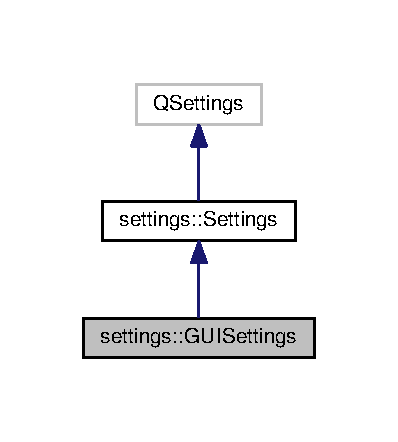
\includegraphics[width=191pt]{classsettings_1_1GUISettings__coll__graph}
\end{center}
\end{figure}
\subsection*{Static Public Member Functions}
\begin{DoxyCompactItemize}
\item 
static \hyperlink{classsettings_1_1GUISettings}{G\+U\+I\+Settings} $\ast$ {\bfseries instance} ()\hypertarget{classsettings_1_1GUISettings_a162cde7ce90582456e4a6ebd998c398d}{}\label{classsettings_1_1GUISettings_a162cde7ce90582456e4a6ebd998c398d}

\end{DoxyCompactItemize}
\subsection*{Additional Inherited Members}


The documentation for this class was generated from the following files\+:\begin{DoxyCompactItemize}
\item 
src/settings/settings.\+h\item 
src/settings/settings.\+cc\end{DoxyCompactItemize}

\hypertarget{classgui_1_1InfoPanel}{}\section{gui\+:\+:Info\+Panel Class Reference}
\label{classgui_1_1InfoPanel}\index{gui\+::\+Info\+Panel@{gui\+::\+Info\+Panel}}


Inheritance diagram for gui\+:\+:Info\+Panel\+:\nopagebreak
\begin{figure}[H]
\begin{center}
\leavevmode
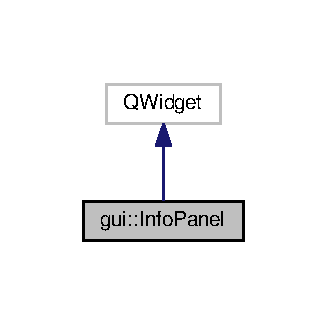
\includegraphics[width=157pt]{classgui_1_1InfoPanel__inherit__graph}
\end{center}
\end{figure}


Collaboration diagram for gui\+:\+:Info\+Panel\+:\nopagebreak
\begin{figure}[H]
\begin{center}
\leavevmode
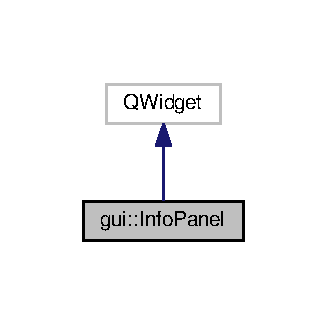
\includegraphics[width=157pt]{classgui_1_1InfoPanel__coll__graph}
\end{center}
\end{figure}
\subsection*{Public Member Functions}
\begin{DoxyCompactItemize}
\item 
{\bfseries Info\+Panel} (Q\+Widget $\ast$parent=0)\hypertarget{classgui_1_1InfoPanel_a6df4d21052d6b3054d4e97841e0e1f3b}{}\label{classgui_1_1InfoPanel_a6df4d21052d6b3054d4e97841e0e1f3b}

\end{DoxyCompactItemize}


The documentation for this class was generated from the following files\+:\begin{DoxyCompactItemize}
\item 
src/gui/widgets/info\+\_\+panel.\+h\item 
src/gui/widgets/info\+\_\+panel.\+cc\end{DoxyCompactItemize}

\hypertarget{classgui_1_1InputField}{}\section{gui\+:\+:Input\+Field Class Reference}
\label{classgui_1_1InputField}\index{gui\+::\+Input\+Field@{gui\+::\+Input\+Field}}


Inheritance diagram for gui\+:\+:Input\+Field\+:\nopagebreak
\begin{figure}[H]
\begin{center}
\leavevmode
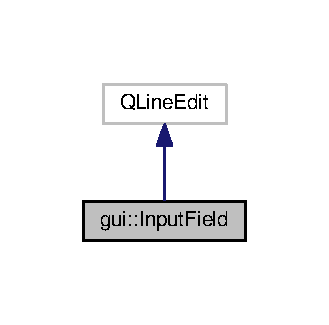
\includegraphics[width=158pt]{classgui_1_1InputField__inherit__graph}
\end{center}
\end{figure}


Collaboration diagram for gui\+:\+:Input\+Field\+:\nopagebreak
\begin{figure}[H]
\begin{center}
\leavevmode
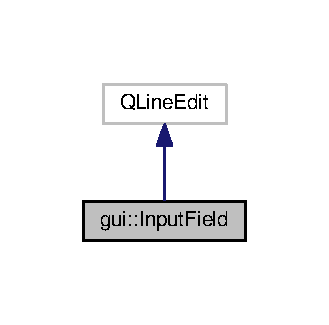
\includegraphics[width=158pt]{classgui_1_1InputField__coll__graph}
\end{center}
\end{figure}
\subsection*{Public Member Functions}
\begin{DoxyCompactItemize}
\item 
{\bfseries Input\+Field} (Q\+Widget $\ast$parent=0)\hypertarget{classgui_1_1InputField_a0b53d1085c2482fdb82d26e47b20efbf}{}\label{classgui_1_1InputField_a0b53d1085c2482fdb82d26e47b20efbf}

\item 
Q\+String {\bfseries pop} ()\hypertarget{classgui_1_1InputField_a620dafdd8938d46b726094b0ffece78e}{}\label{classgui_1_1InputField_a620dafdd8938d46b726094b0ffece78e}

\end{DoxyCompactItemize}


The documentation for this class was generated from the following files\+:\begin{DoxyCompactItemize}
\item 
src/gui/widgets/input\+\_\+field.\+h\item 
src/gui/widgets/input\+\_\+field.\+cc\end{DoxyCompactItemize}

\hypertarget{classprim_1_1Item}{}\section{prim\+:\+:Item Class Reference}
\label{classprim_1_1Item}\index{prim\+::\+Item@{prim\+::\+Item}}


Customized Q\+Graphics\+Item subclass. All items in the Layers must inherit this class and should be distinguished by the item\+\_\+type member. Both bounding\+Rect and paint must be redefined in any derived classes.  




{\ttfamily \#include $<$item.\+h$>$}



Inheritance diagram for prim\+:\+:Item\+:\nopagebreak
\begin{figure}[H]
\begin{center}
\leavevmode
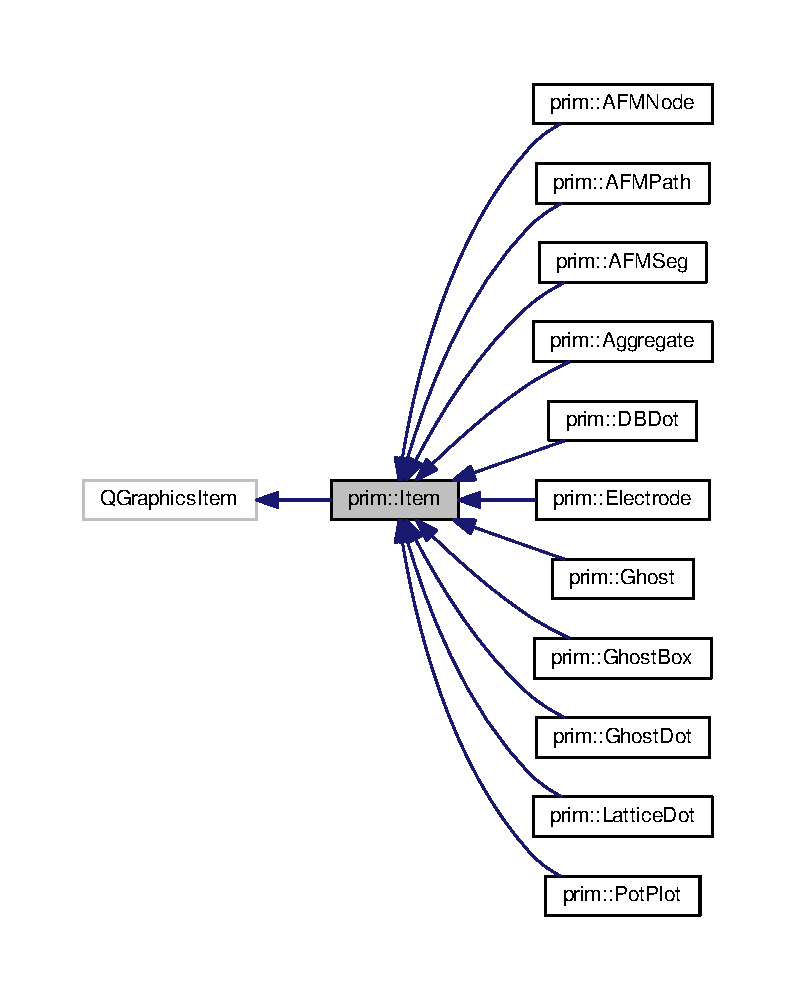
\includegraphics[width=350pt]{classprim_1_1Item__inherit__graph}
\end{center}
\end{figure}


Collaboration diagram for prim\+:\+:Item\+:\nopagebreak
\begin{figure}[H]
\begin{center}
\leavevmode
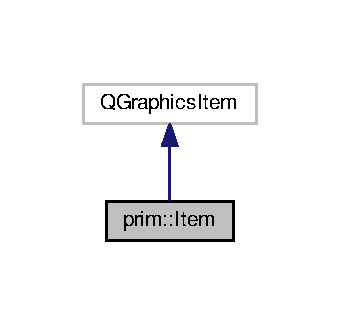
\includegraphics[width=163pt]{classprim_1_1Item__coll__graph}
\end{center}
\end{figure}
\subsection*{Public Types}
\begin{DoxyCompactItemize}
\item 
enum \hyperlink{classprim_1_1Item_a5c096201e92c0b15a62c7af1cff1d79c}{Item\+Type} \{ \\*
{\bfseries Aggregate}, 
{\bfseries D\+B\+Dot}, 
{\bfseries Lattice\+Dot}, 
{\bfseries Ghost}, 
\\*
{\bfseries Ghost\+Dot}, 
{\bfseries Text}, 
{\bfseries Electrode}, 
{\bfseries Ghost\+Box}, 
\\*
{\bfseries A\+F\+M\+Path}, 
{\bfseries A\+F\+M\+Node}, 
{\bfseries A\+F\+M\+Seg}, 
{\bfseries Pot\+Plot}
 \}\hypertarget{classprim_1_1Item_a5c096201e92c0b15a62c7af1cff1d79c}{}\label{classprim_1_1Item_a5c096201e92c0b15a62c7af1cff1d79c}
\begin{DoxyCompactList}\small\item\em Every derived class should be assigned an enumerated label in order to distinguish them in functions which accept \hyperlink{classprim_1_1Item}{Item} objects. Derived classes can be declared and implemented elsewhere as long as they are defined before use. \end{DoxyCompactList}
\end{DoxyCompactItemize}
\subsection*{Public Member Functions}
\begin{DoxyCompactItemize}
\item 
\hyperlink{classprim_1_1Item_aea18693709a1a1e68ff7c850ddac4f8d}{Item} (\hyperlink{classprim_1_1Item_a5c096201e92c0b15a62c7af1cff1d79c}{Item\+Type} type, int lay\+\_\+id=-\/1, Q\+Graphics\+Item $\ast$parent=0)\hypertarget{classprim_1_1Item_aea18693709a1a1e68ff7c850ddac4f8d}{}\label{classprim_1_1Item_aea18693709a1a1e68ff7c850ddac4f8d}

\begin{DoxyCompactList}\small\item\em constructor, layer = 0 should indicate temporary objects that do not belong to any particular layer \end{DoxyCompactList}\item 
\hyperlink{classprim_1_1Item_abd1264482c7ac14a624e47f7055361f7}{$\sim$\+Item} ()\hypertarget{classprim_1_1Item_abd1264482c7ac14a624e47f7055361f7}{}\label{classprim_1_1Item_abd1264482c7ac14a624e47f7055361f7}

\begin{DoxyCompactList}\small\item\em destructor \end{DoxyCompactList}\item 
void \hyperlink{classprim_1_1Item_af7d21525ff40264b8802313e2bfe7c92}{set\+Layer\+Index} (int lay\+\_\+id)\hypertarget{classprim_1_1Item_af7d21525ff40264b8802313e2bfe7c92}{}\label{classprim_1_1Item_af7d21525ff40264b8802313e2bfe7c92}

\begin{DoxyCompactList}\small\item\em update layer\+\_\+id \end{DoxyCompactList}\item 
virtual Q\+RectF {\bfseries bounding\+Rect} () const =0\hypertarget{classprim_1_1Item_ac02889fb453cf3b2609abce18aa1f855}{}\label{classprim_1_1Item_ac02889fb453cf3b2609abce18aa1f855}

\item 
virtual void {\bfseries paint} (Q\+Painter $\ast$, const Q\+Style\+Option\+Graphics\+Item $\ast$, Q\+Widget $\ast$)=0\hypertarget{classprim_1_1Item_a4d33b3693d3c055822b62f97fa0b6b2e}{}\label{classprim_1_1Item_a4d33b3693d3c055822b62f97fa0b6b2e}

\item 
virtual \hyperlink{classprim_1_1Item}{Item} $\ast$ \hyperlink{classprim_1_1Item_a8852183d5198ef3af3f2fa394dfc0789}{deep\+Copy} () const =0\hypertarget{classprim_1_1Item_a8852183d5198ef3af3f2fa394dfc0789}{}\label{classprim_1_1Item_a8852183d5198ef3af3f2fa394dfc0789}

\begin{DoxyCompactList}\small\item\em create a deep copy of the \hyperlink{classprim_1_1Item}{Item} for the clipboard. Deep-\/copied items should have no parent or scene and need only to have the information necessary to create a new copy somewhere in the scene \end{DoxyCompactList}\item 
bool \hyperlink{classprim_1_1Item_aa27c998ca6ace4bb07fbff3ad522c37f}{up\+Selected} ()\hypertarget{classprim_1_1Item_aa27c998ca6ace4bb07fbff3ad522c37f}{}\label{classprim_1_1Item_aa27c998ca6ace4bb07fbff3ad522c37f}

\begin{DoxyCompactList}\small\item\em true if the item or its parent has been seleted, recursive to highest level parent \end{DoxyCompactList}\item 
void \hyperlink{classprim_1_1Item_a58b962da55176665e1e53c735f2d3e08}{set\+Hovered} (bool flag)\hypertarget{classprim_1_1Item_a58b962da55176665e1e53c735f2d3e08}{}\label{classprim_1_1Item_a58b962da55176665e1e53c735f2d3e08}

\begin{DoxyCompactList}\small\item\em set hovered state \end{DoxyCompactList}\item 
bool \hyperlink{classprim_1_1Item_a1fc8c6d8a6f62c3e26dc41516d6bb881}{is\+Hovered} ()\hypertarget{classprim_1_1Item_a1fc8c6d8a6f62c3e26dc41516d6bb881}{}\label{classprim_1_1Item_a1fc8c6d8a6f62c3e26dc41516d6bb881}

\begin{DoxyCompactList}\small\item\em get hovered state \end{DoxyCompactList}\item 
bool \hyperlink{classprim_1_1Item_ab6ae17ce9ed2b54fabc9f6016ea0c4e0}{up\+Hovered} ()\hypertarget{classprim_1_1Item_ab6ae17ce9ed2b54fabc9f6016ea0c4e0}{}\label{classprim_1_1Item_ab6ae17ce9ed2b54fabc9f6016ea0c4e0}

\begin{DoxyCompactList}\small\item\em true if the item or its parent has been hovered, recursive to highest level parent \end{DoxyCompactList}\item 
void \hyperlink{classprim_1_1Item_a6384844cdf9abf96f07197e0e654ad0d}{set\+Design\+Mode} (bool mode)\hypertarget{classprim_1_1Item_a6384844cdf9abf96f07197e0e654ad0d}{}\label{classprim_1_1Item_a6384844cdf9abf96f07197e0e654ad0d}

\begin{DoxyCompactList}\small\item\em set design mode \end{DoxyCompactList}\item 
bool \hyperlink{classprim_1_1Item_abbd09ee53e8c057184f2c2e702496059}{design\+Mode} ()\hypertarget{classprim_1_1Item_abbd09ee53e8c057184f2c2e702496059}{}\label{classprim_1_1Item_abbd09ee53e8c057184f2c2e702496059}

\begin{DoxyCompactList}\small\item\em get design mode \end{DoxyCompactList}\item 
virtual void {\bfseries save\+Items} (Q\+Xml\+Stream\+Writer $\ast$) const \hypertarget{classprim_1_1Item_ae336707c628f8f5079a5bc60a599e513}{}\label{classprim_1_1Item_ae336707c628f8f5079a5bc60a599e513}

\item 
virtual void {\bfseries load\+From\+File} (Q\+Xml\+Stream\+Reader $\ast$)\hypertarget{classprim_1_1Item_a35f7e8f106e8263f059700a8f63c7728}{}\label{classprim_1_1Item_a35f7e8f106e8263f059700a8f63c7728}

\end{DoxyCompactItemize}
\subsection*{Static Public Member Functions}
\begin{DoxyCompactItemize}
\item 
static void {\bfseries init} ()\hypertarget{classprim_1_1Item_a1714fdab34f3fd64f897e73deabb7c01}{}\label{classprim_1_1Item_a1714fdab34f3fd64f897e73deabb7c01}

\end{DoxyCompactItemize}
\subsection*{Public Attributes}
\begin{DoxyCompactItemize}
\item 
\hyperlink{classprim_1_1Item_a5c096201e92c0b15a62c7af1cff1d79c}{Item\+Type} {\bfseries item\+\_\+type}\hypertarget{classprim_1_1Item_ad8df001372c1ee5bba97beab8dd27058}{}\label{classprim_1_1Item_ad8df001372c1ee5bba97beab8dd27058}

\item 
int {\bfseries layer\+\_\+id}\hypertarget{classprim_1_1Item_af3678c770be3b1670cf0a90f04bb11f4}{}\label{classprim_1_1Item_af3678c770be3b1670cf0a90f04bb11f4}

\end{DoxyCompactItemize}
\subsection*{Static Public Attributes}
\begin{DoxyCompactItemize}
\item 
static qreal {\bfseries scale\+\_\+factor} = -\/1\hypertarget{classprim_1_1Item_ad933d2f7bd50855e185b5b40892bf443}{}\label{classprim_1_1Item_ad933d2f7bd50855e185b5b40892bf443}

\item 
static bool {\bfseries select\+\_\+mode} = false\hypertarget{classprim_1_1Item_a5fa9c62bd2ec8f1817b29c42e351c6a3}{}\label{classprim_1_1Item_a5fa9c62bd2ec8f1817b29c42e351c6a3}

\item 
static bool {\bfseries db\+\_\+gen\+\_\+mode} = false\hypertarget{classprim_1_1Item_a0bfa8382e489fe7a34da66b1a61ba8a4}{}\label{classprim_1_1Item_a0bfa8382e489fe7a34da66b1a61ba8a4}

\item 
static bool {\bfseries electrode\+\_\+mode} = false\hypertarget{classprim_1_1Item_ad75df406c06999ff2fe13696a45d5677}{}\label{classprim_1_1Item_ad75df406c06999ff2fe13696a45d5677}

\end{DoxyCompactItemize}
\subsection*{Protected Member Functions}
\begin{DoxyCompactItemize}
\item 
virtual void {\bfseries mouse\+Press\+Event} (Q\+Graphics\+Scene\+Mouse\+Event $\ast$) Q\+\_\+\+D\+E\+C\+L\+\_\+\+O\+V\+E\+R\+R\+I\+DE\hypertarget{classprim_1_1Item_a75a1a4b6f81ebd0fd0645a6c5edb254c}{}\label{classprim_1_1Item_a75a1a4b6f81ebd0fd0645a6c5edb254c}

\item 
virtual void {\bfseries hover\+Enter\+Event} (Q\+Graphics\+Scene\+Hover\+Event $\ast$) Q\+\_\+\+D\+E\+C\+L\+\_\+\+O\+V\+E\+R\+R\+I\+DE\hypertarget{classprim_1_1Item_a525884955272aa10a485b5e98b21ff9f}{}\label{classprim_1_1Item_a525884955272aa10a485b5e98b21ff9f}

\item 
virtual void {\bfseries hover\+Leave\+Event} (Q\+Graphics\+Scene\+Hover\+Event $\ast$) Q\+\_\+\+D\+E\+C\+L\+\_\+\+O\+V\+E\+R\+R\+I\+DE\hypertarget{classprim_1_1Item_aeb2f8ca4597c824cb58c3ae7092624ed}{}\label{classprim_1_1Item_aeb2f8ca4597c824cb58c3ae7092624ed}

\end{DoxyCompactItemize}
\subsection*{Protected Attributes}
\begin{DoxyCompactItemize}
\item 
bool \hyperlink{classprim_1_1Item_a36459a945e47fc3acd2c4aeeba1bfa35}{hovered}\hypertarget{classprim_1_1Item_a36459a945e47fc3acd2c4aeeba1bfa35}{}\label{classprim_1_1Item_a36459a945e47fc3acd2c4aeeba1bfa35}

\begin{DoxyCompactList}\small\item\em manipulated through \hyperlink{classprim_1_1Item_a58b962da55176665e1e53c735f2d3e08}{set\+Hovered(bool)} and \hyperlink{classprim_1_1Item_a36459a945e47fc3acd2c4aeeba1bfa35}{hovered()} \end{DoxyCompactList}\end{DoxyCompactItemize}


\subsection{Detailed Description}
Customized Q\+Graphics\+Item subclass. All items in the Layers must inherit this class and should be distinguished by the item\+\_\+type member. Both bounding\+Rect and paint must be redefined in any derived classes. 

The documentation for this class was generated from the following files\+:\begin{DoxyCompactItemize}
\item 
src/gui/widgets/primitives/\hyperlink{item_8h}{item.\+h}\item 
src/gui/widgets/primitives/item.\+cc\end{DoxyCompactItemize}

\hypertarget{classprim_1_1Lattice}{}\section{prim\+:\+:Lattice Class Reference}
\label{classprim_1_1Lattice}\index{prim\+::\+Lattice@{prim\+::\+Lattice}}


Inheritance diagram for prim\+:\+:Lattice\+:\nopagebreak
\begin{figure}[H]
\begin{center}
\leavevmode
\includegraphics[width=151pt]{classprim_1_1Lattice__inherit__graph}
\end{center}
\end{figure}


Collaboration diagram for prim\+:\+:Lattice\+:\nopagebreak
\begin{figure}[H]
\begin{center}
\leavevmode
\includegraphics[width=151pt]{classprim_1_1Lattice__coll__graph}
\end{center}
\end{figure}
\subsection*{Public Member Functions}
\begin{DoxyCompactItemize}
\item 
\hyperlink{classprim_1_1Lattice_a2ee0efb9189cbd53d39be3733cedcac0}{Lattice} (const Q\+String \&fname=Q\+String(), int lay\+\_\+id=-\/1)\hypertarget{classprim_1_1Lattice_a2ee0efb9189cbd53d39be3733cedcac0}{}\label{classprim_1_1Lattice_a2ee0efb9189cbd53d39be3733cedcac0}

\begin{DoxyCompactList}\small\item\em constructor \end{DoxyCompactList}\item 
\hyperlink{classprim_1_1Lattice_a054bbc6c783c4d2128380e47ccbdf8ef}{$\sim$\+Lattice} ()\hypertarget{classprim_1_1Lattice_a054bbc6c783c4d2128380e47ccbdf8ef}{}\label{classprim_1_1Lattice_a054bbc6c783c4d2128380e47ccbdf8ef}

\begin{DoxyCompactList}\small\item\em destructor \end{DoxyCompactList}\end{DoxyCompactItemize}
\subsection*{Additional Inherited Members}


The documentation for this class was generated from the following files\+:\begin{DoxyCompactItemize}
\item 
src/gui/widgets/primitives/\hyperlink{lattice_8h}{lattice.\+h}\item 
src/gui/widgets/primitives/lattice.\+cc\end{DoxyCompactItemize}

\hypertarget{classprim_1_1LatticeDot}{}\section{prim\+:\+:Lattice\+Dot Class Reference}
\label{classprim_1_1LatticeDot}\index{prim\+::\+Lattice\+Dot@{prim\+::\+Lattice\+Dot}}


Specific \hyperlink{classprim_1_1Item}{Item} derived class for showing the possible dangling bond location on the surface lattice. For now, this class has very similar characteristics to the \hyperlink{classprim_1_1DBDot}{D\+B\+Dot} but will be kept a separate class to allow for future distinction in properties and avoid overbloating the functionality of either class.  




{\ttfamily \#include $<$latdot.\+h$>$}



Inheritance diagram for prim\+:\+:Lattice\+Dot\+:\nopagebreak
\begin{figure}[H]
\begin{center}
\leavevmode
\includegraphics[width=166pt]{classprim_1_1LatticeDot__inherit__graph}
\end{center}
\end{figure}


Collaboration diagram for prim\+:\+:Lattice\+Dot\+:\nopagebreak
\begin{figure}[H]
\begin{center}
\leavevmode
\includegraphics[width=166pt]{classprim_1_1LatticeDot__coll__graph}
\end{center}
\end{figure}
\subsection*{Public Member Functions}
\begin{DoxyCompactItemize}
\item 
\hyperlink{classprim_1_1LatticeDot_ad4dfe6d2c15e4cd9f291003845820950}{Lattice\+Dot} (int layer\+\_\+id, Q\+PointF p\+\_\+loc)\hypertarget{classprim_1_1LatticeDot_ad4dfe6d2c15e4cd9f291003845820950}{}\label{classprim_1_1LatticeDot_ad4dfe6d2c15e4cd9f291003845820950}

\begin{DoxyCompactList}\small\item\em constructor, create a lattice dot at the given location in physical units \end{DoxyCompactList}\item 
\hyperlink{classprim_1_1LatticeDot_a2e3c21e2ff61dc41aaec30d1e7a94ae1}{$\sim$\+Lattice\+Dot} ()\hypertarget{classprim_1_1LatticeDot_a2e3c21e2ff61dc41aaec30d1e7a94ae1}{}\label{classprim_1_1LatticeDot_a2e3c21e2ff61dc41aaec30d1e7a94ae1}

\begin{DoxyCompactList}\small\item\em destructor \end{DoxyCompactList}\item 
Q\+PointF \hyperlink{classprim_1_1LatticeDot_aa11ad28b8d3524622e686e4f2c6aa5ee}{get\+Phys\+Loc} () const \hypertarget{classprim_1_1LatticeDot_aa11ad28b8d3524622e686e4f2c6aa5ee}{}\label{classprim_1_1LatticeDot_aa11ad28b8d3524622e686e4f2c6aa5ee}

\begin{DoxyCompactList}\small\item\em get the dots physical location \end{DoxyCompactList}\item 
\hyperlink{classprim_1_1DBDot}{prim\+::\+D\+B\+Dot} $\ast$ \hyperlink{classprim_1_1LatticeDot_a88d99a155ee489d376377441a041c709}{get\+D\+B\+Dot} () const \hypertarget{classprim_1_1LatticeDot_a88d99a155ee489d376377441a041c709}{}\label{classprim_1_1LatticeDot_a88d99a155ee489d376377441a041c709}

\begin{DoxyCompactList}\small\item\em get the created dangling bond \end{DoxyCompactList}\item 
void \hyperlink{classprim_1_1LatticeDot_a2c0cc2994be5dd8f23d7b2e832a88e8f}{set\+D\+B\+Dot} (\hyperlink{classprim_1_1DBDot}{prim\+::\+D\+B\+Dot} $\ast$dot=0)\hypertarget{classprim_1_1LatticeDot_a2c0cc2994be5dd8f23d7b2e832a88e8f}{}\label{classprim_1_1LatticeDot_a2c0cc2994be5dd8f23d7b2e832a88e8f}

\begin{DoxyCompactList}\small\item\em set the created dangling bond \end{DoxyCompactList}\item 
Q\+RectF {\bfseries bounding\+Rect} () const Q\+\_\+\+D\+E\+C\+L\+\_\+\+O\+V\+E\+R\+R\+I\+DE\hypertarget{classprim_1_1LatticeDot_a0ffa32428b40778903c3ec86ee9a0df1}{}\label{classprim_1_1LatticeDot_a0ffa32428b40778903c3ec86ee9a0df1}

\item 
void {\bfseries paint} (Q\+Painter $\ast$, const Q\+Style\+Option\+Graphics\+Item $\ast$, Q\+Widget $\ast$) Q\+\_\+\+D\+E\+C\+L\+\_\+\+O\+V\+E\+R\+R\+I\+DE\hypertarget{classprim_1_1LatticeDot_a91aaa7de48bcf0be8bbf598fc23b74f8}{}\label{classprim_1_1LatticeDot_a91aaa7de48bcf0be8bbf598fc23b74f8}

\item 
\hyperlink{classprim_1_1Item}{Item} $\ast$ \hyperlink{classprim_1_1LatticeDot_af47222050d9b850de87a4d9921bc9db7}{deep\+Copy} () const \hypertarget{classprim_1_1LatticeDot_af47222050d9b850de87a4d9921bc9db7}{}\label{classprim_1_1LatticeDot_af47222050d9b850de87a4d9921bc9db7}

\begin{DoxyCompactList}\small\item\em create a deep copy of the \hyperlink{classprim_1_1Item}{Item} for the clipboard. Deep-\/copied items should have no parent or scene and need only to have the information necessary to create a new copy somewhere in the scene \end{DoxyCompactList}\end{DoxyCompactItemize}
\subsection*{Protected Member Functions}
\begin{DoxyCompactItemize}
\item 
virtual void {\bfseries mouse\+Double\+Click\+Event} (Q\+Graphics\+Scene\+Mouse\+Event $\ast$e) Q\+\_\+\+D\+E\+C\+L\+\_\+\+O\+V\+E\+R\+R\+I\+DE\hypertarget{classprim_1_1LatticeDot_a09eb56de975cdd92bb80cf7d661b4e57}{}\label{classprim_1_1LatticeDot_a09eb56de975cdd92bb80cf7d661b4e57}

\end{DoxyCompactItemize}
\subsection*{Additional Inherited Members}


\subsection{Detailed Description}
Specific \hyperlink{classprim_1_1Item}{Item} derived class for showing the possible dangling bond location on the surface lattice. For now, this class has very similar characteristics to the \hyperlink{classprim_1_1DBDot}{D\+B\+Dot} but will be kept a separate class to allow for future distinction in properties and avoid overbloating the functionality of either class. 

The documentation for this class was generated from the following files\+:\begin{DoxyCompactItemize}
\item 
src/gui/widgets/primitives/\hyperlink{latdot_8h}{latdot.\+h}\item 
src/gui/widgets/primitives/latdot.\+cc\end{DoxyCompactItemize}

\hypertarget{classsettings_1_1LatticeSettings}{}\section{settings\+:\+:Lattice\+Settings Class Reference}
\label{classsettings_1_1LatticeSettings}\index{settings\+::\+Lattice\+Settings@{settings\+::\+Lattice\+Settings}}


Inheritance diagram for settings\+:\+:Lattice\+Settings\+:\nopagebreak
\begin{figure}[H]
\begin{center}
\leavevmode
\includegraphics[width=202pt]{classsettings_1_1LatticeSettings__inherit__graph}
\end{center}
\end{figure}


Collaboration diagram for settings\+:\+:Lattice\+Settings\+:\nopagebreak
\begin{figure}[H]
\begin{center}
\leavevmode
\includegraphics[width=202pt]{classsettings_1_1LatticeSettings__coll__graph}
\end{center}
\end{figure}
\subsection*{Static Public Member Functions}
\begin{DoxyCompactItemize}
\item 
static \hyperlink{classsettings_1_1LatticeSettings}{Lattice\+Settings} $\ast$ {\bfseries instance} ()\hypertarget{classsettings_1_1LatticeSettings_a6c7a45857ec492e8295924cfb427336e}{}\label{classsettings_1_1LatticeSettings_a6c7a45857ec492e8295924cfb427336e}

\item 
static void {\bfseries update\+Lattice} (const Q\+String \&fname=Q\+String())\hypertarget{classsettings_1_1LatticeSettings_aa2018ab5eae604c135163a95abf42b53}{}\label{classsettings_1_1LatticeSettings_aa2018ab5eae604c135163a95abf42b53}

\end{DoxyCompactItemize}
\subsection*{Additional Inherited Members}


The documentation for this class was generated from the following files\+:\begin{DoxyCompactItemize}
\item 
src/settings/settings.\+h\item 
src/settings/settings.\+cc\end{DoxyCompactItemize}

\hypertarget{classprim_1_1Layer}{}\section{prim\+:\+:Layer Class Reference}
\label{classprim_1_1Layer}\index{prim\+::\+Layer@{prim\+::\+Layer}}


Base Class for design layers, layers do not delete their items when destroyed.  




{\ttfamily \#include $<$layer.\+h$>$}



Inheritance diagram for prim\+:\+:Layer\+:\nopagebreak
\begin{figure}[H]
\begin{center}
\leavevmode
\includegraphics[width=151pt]{classprim_1_1Layer__inherit__graph}
\end{center}
\end{figure}


Collaboration diagram for prim\+:\+:Layer\+:\nopagebreak
\begin{figure}[H]
\begin{center}
\leavevmode
\includegraphics[width=145pt]{classprim_1_1Layer__coll__graph}
\end{center}
\end{figure}
\subsection*{Public Types}
\begin{DoxyCompactItemize}
\item 
enum \hyperlink{classprim_1_1Layer_a9a9c22ae767c4671a07293b69c540547}{Layer\+Type} \{ \\*
{\bfseries Lattice}, 
{\bfseries DB}, 
{\bfseries Electrode}, 
{\bfseries A\+F\+M\+Tip}, 
\\*
{\bfseries Plot}
 \}\hypertarget{classprim_1_1Layer_a9a9c22ae767c4671a07293b69c540547}{}\label{classprim_1_1Layer_a9a9c22ae767c4671a07293b69c540547}
\begin{DoxyCompactList}\small\item\em enum type for different layer contents \end{DoxyCompactList}
\end{DoxyCompactItemize}
\subsection*{Public Slots}
\begin{DoxyCompactItemize}
\item 
void {\bfseries visibility\+Check\+Box\+Changed} (int check\+\_\+state)\hypertarget{classprim_1_1Layer_a107df2ecd3c62a8a2850ab16b259cd97}{}\label{classprim_1_1Layer_a107df2ecd3c62a8a2850ab16b259cd97}

\item 
void {\bfseries visibility\+Push\+Button\+Changed} (bool checked)\hypertarget{classprim_1_1Layer_aff089bee001dceb4a6ef0d8bdc46c18b}{}\label{classprim_1_1Layer_aff089bee001dceb4a6ef0d8bdc46c18b}

\item 
void {\bfseries editability\+Push\+Button\+Changed} (bool checked)\hypertarget{classprim_1_1Layer_aadf868aa24684752991db0354f01fed9}{}\label{classprim_1_1Layer_aadf868aa24684752991db0354f01fed9}

\end{DoxyCompactItemize}
\subsection*{Public Member Functions}
\begin{DoxyCompactItemize}
\item 
\hyperlink{classprim_1_1Layer_a0aa88b44c1ca33a9fb37048d1955e9e4}{Layer} (const Q\+String \&nm=Q\+String(), const \hyperlink{classprim_1_1Layer_a9a9c22ae767c4671a07293b69c540547}{Layer\+Type} cnt\+\_\+type=DB, const float z\+\_\+offset=0, const float z\+\_\+height=0, int lay\+\_\+id=-\/1, Q\+Object $\ast$parent=0)\hypertarget{classprim_1_1Layer_a0aa88b44c1ca33a9fb37048d1955e9e4}{}\label{classprim_1_1Layer_a0aa88b44c1ca33a9fb37048d1955e9e4}

\begin{DoxyCompactList}\small\item\em constructor, create a \hyperlink{classprim_1_1Layer}{Layer} with the given name. If no name is given, use the default naming scheme with layer\+\_\+count. \end{DoxyCompactList}\item 
\hyperlink{classprim_1_1Layer_adcfacc407024def1aba20b83337209d1}{Layer} (Q\+Xml\+Stream\+Reader $\ast$stream)\hypertarget{classprim_1_1Layer_adcfacc407024def1aba20b83337209d1}{}\label{classprim_1_1Layer_adcfacc407024def1aba20b83337209d1}

\begin{DoxyCompactList}\small\item\em constructor, create a \hyperlink{classprim_1_1Layer}{Layer} from the design file. \end{DoxyCompactList}\item 
void \hyperlink{classprim_1_1Layer_a7a49a82ff912a32d028352b48784ae1a}{set\+Layer\+Index} (int lay\+\_\+id)\hypertarget{classprim_1_1Layer_a7a49a82ff912a32d028352b48784ae1a}{}\label{classprim_1_1Layer_a7a49a82ff912a32d028352b48784ae1a}

\begin{DoxyCompactList}\small\item\em set layer index and update layer\+\_\+id of contained items \end{DoxyCompactList}\item 
void \hyperlink{classprim_1_1Layer_aa9ab5f693f5f2526b34422b5c29606d7}{set\+Z\+Offset} (const float z\+\_\+offset)\hypertarget{classprim_1_1Layer_aa9ab5f693f5f2526b34422b5c29606d7}{}\label{classprim_1_1Layer_aa9ab5f693f5f2526b34422b5c29606d7}

\begin{DoxyCompactList}\small\item\em set the zoffset of the layer \end{DoxyCompactList}\item 
float \hyperlink{classprim_1_1Layer_a7ae3cbed96ce075e56e444538805ed09}{z\+Offset} ()\hypertarget{classprim_1_1Layer_a7ae3cbed96ce075e56e444538805ed09}{}\label{classprim_1_1Layer_a7ae3cbed96ce075e56e444538805ed09}

\begin{DoxyCompactList}\small\item\em get the zoffset of the layer \end{DoxyCompactList}\item 
void \hyperlink{classprim_1_1Layer_a5947e3dc1ad3a3d7657b6bf7cc3ed439}{set\+Z\+Height} (const float z\+\_\+height)\hypertarget{classprim_1_1Layer_a5947e3dc1ad3a3d7657b6bf7cc3ed439}{}\label{classprim_1_1Layer_a5947e3dc1ad3a3d7657b6bf7cc3ed439}

\begin{DoxyCompactList}\small\item\em set the zheight of the layer \end{DoxyCompactList}\item 
float \hyperlink{classprim_1_1Layer_a04fba2a5c8347f7a249b28018581018f}{z\+Height} ()\hypertarget{classprim_1_1Layer_a04fba2a5c8347f7a249b28018581018f}{}\label{classprim_1_1Layer_a04fba2a5c8347f7a249b28018581018f}

\begin{DoxyCompactList}\small\item\em get the zheight of the layer \end{DoxyCompactList}\item 
void \hyperlink{classprim_1_1Layer_a688a2d06a43c128f9e98dc60e3b0157e}{add\+Item} (\hyperlink{classprim_1_1Item}{prim\+::\+Item} $\ast$item, int index=-\/1)\hypertarget{classprim_1_1Layer_a688a2d06a43c128f9e98dc60e3b0157e}{}\label{classprim_1_1Layer_a688a2d06a43c128f9e98dc60e3b0157e}

\begin{DoxyCompactList}\small\item\em add a new \hyperlink{classprim_1_1Item}{Item} to the current layer. If the \hyperlink{classprim_1_1Item}{Item} is already in the layer, do nothing. \end{DoxyCompactList}\item 
bool \hyperlink{classprim_1_1Layer_a760643f11d83c0c9f841de211787f7cc}{remove\+Item} (\hyperlink{classprim_1_1Item}{prim\+::\+Item} $\ast$item)\hypertarget{classprim_1_1Layer_a760643f11d83c0c9f841de211787f7cc}{}\label{classprim_1_1Layer_a760643f11d83c0c9f841de211787f7cc}

\begin{DoxyCompactList}\small\item\em attempt to remove the given \hyperlink{classprim_1_1Item}{Item} from the layer. Returns true if the \hyperlink{classprim_1_1Item}{Item} is found and removed, false otherwise. \end{DoxyCompactList}\item 
\hyperlink{classprim_1_1Item}{prim\+::\+Item} $\ast$ \hyperlink{classprim_1_1Layer_ad8ab05f2dc4eb37b3cb1b58ce465e9d9}{take\+Item} (int ind=-\/1)\hypertarget{classprim_1_1Layer_ad8ab05f2dc4eb37b3cb1b58ce465e9d9}{}\label{classprim_1_1Layer_ad8ab05f2dc4eb37b3cb1b58ce465e9d9}

\begin{DoxyCompactList}\small\item\em pop the \hyperlink{classprim_1_1Item}{Item} given by the index. Returns 0 if invalid index. \end{DoxyCompactList}\item 
void \hyperlink{classprim_1_1Layer_aa9ec922e6147d213b7a391f23e2fe764}{set\+Visible} (bool vis)\hypertarget{classprim_1_1Layer_aa9ec922e6147d213b7a391f23e2fe764}{}\label{classprim_1_1Layer_aa9ec922e6147d213b7a391f23e2fe764}

\begin{DoxyCompactList}\small\item\em update the layer visibility, calls set\+Visible(vis) for all Items in the layer. If vis==visibility, do nothing. \end{DoxyCompactList}\item 
bool \hyperlink{classprim_1_1Layer_a6fff1ee8d18b3d7951277dddffb89257}{is\+Visible} () const \hypertarget{classprim_1_1Layer_a6fff1ee8d18b3d7951277dddffb89257}{}\label{classprim_1_1Layer_a6fff1ee8d18b3d7951277dddffb89257}

\begin{DoxyCompactList}\small\item\em check if the layer should be visible \end{DoxyCompactList}\item 
void \hyperlink{classprim_1_1Layer_af7e5d87a863fa06328ec71473f6a4910}{set\+Active} (bool act)\hypertarget{classprim_1_1Layer_af7e5d87a863fa06328ec71473f6a4910}{}\label{classprim_1_1Layer_af7e5d87a863fa06328ec71473f6a4910}

\begin{DoxyCompactList}\small\item\em update the layer activity, calls set\+Active(act) for all Items in the layer \end{DoxyCompactList}\item 
bool \hyperlink{classprim_1_1Layer_af2e5a5c51de236881c68a7dbfafe4d77}{is\+Active} () const \hypertarget{classprim_1_1Layer_af2e5a5c51de236881c68a7dbfafe4d77}{}\label{classprim_1_1Layer_af2e5a5c51de236881c68a7dbfafe4d77}

\begin{DoxyCompactList}\small\item\em check if the layer should be active \end{DoxyCompactList}\item 
const Q\+String \& \hyperlink{classprim_1_1Layer_aba036a8f047a91e7629f81130bbcb7bb}{get\+Name} () const \hypertarget{classprim_1_1Layer_aba036a8f047a91e7629f81130bbcb7bb}{}\label{classprim_1_1Layer_aba036a8f047a91e7629f81130bbcb7bb}

\begin{DoxyCompactList}\small\item\em get the \hyperlink{classprim_1_1Layer}{Layer} name, possibly change return to const Q\+String\& \end{DoxyCompactList}\item 
void \hyperlink{classprim_1_1Layer_a477672eee633e7a908abdc3648905d74}{set\+Content\+Type} (\hyperlink{classprim_1_1Layer_a9a9c22ae767c4671a07293b69c540547}{Layer\+Type} type)\hypertarget{classprim_1_1Layer_a477672eee633e7a908abdc3648905d74}{}\label{classprim_1_1Layer_a477672eee633e7a908abdc3648905d74}

\begin{DoxyCompactList}\small\item\em set the \hyperlink{classprim_1_1Layer}{Layer} content type \end{DoxyCompactList}\item 
\hyperlink{classprim_1_1Layer_a9a9c22ae767c4671a07293b69c540547}{Layer\+Type} \hyperlink{classprim_1_1Layer_af009cb8e716255926c14abea588a8362}{get\+Content\+Type} ()\hypertarget{classprim_1_1Layer_af009cb8e716255926c14abea588a8362}{}\label{classprim_1_1Layer_af009cb8e716255926c14abea588a8362}

\begin{DoxyCompactList}\small\item\em get the \hyperlink{classprim_1_1Layer}{Layer} content type, like \char`\"{}electrode\char`\"{}, \char`\"{}dbdots\char`\"{}, etc. \end{DoxyCompactList}\item 
const Q\+String {\bfseries get\+Content\+Type\+String} () const \hypertarget{classprim_1_1Layer_aa98e5ea74d0d956e06f71ab07c15903a}{}\label{classprim_1_1Layer_aa98e5ea74d0d956e06f71ab07c15903a}

\item 
\hyperlink{classprim_1_1Item}{prim\+::\+Item} $\ast$ \hyperlink{classprim_1_1Layer_a1d2ef0cb4f5607b1768f9b23bad42d24}{get\+Item} (int i)\hypertarget{classprim_1_1Layer_a1d2ef0cb4f5607b1768f9b23bad42d24}{}\label{classprim_1_1Layer_a1d2ef0cb4f5607b1768f9b23bad42d24}

\begin{DoxyCompactList}\small\item\em if i is within bounds, return a pointer to the indexed item in the \hyperlink{classprim_1_1Layer}{Layer} item stack; otherwise, return 0 \end{DoxyCompactList}\item 
int \hyperlink{classprim_1_1Layer_a071458923f67767d195db5b5648fa319}{get\+Item\+Index} (\hyperlink{classprim_1_1Item}{prim\+::\+Item} $\ast$item)\hypertarget{classprim_1_1Layer_a071458923f67767d195db5b5648fa319}{}\label{classprim_1_1Layer_a071458923f67767d195db5b5648fa319}

\begin{DoxyCompactList}\small\item\em get index of an item with the item\textquotesingle{}s pointer \end{DoxyCompactList}\item 
Q\+Stack$<$ \hyperlink{classprim_1_1Item}{prim\+::\+Item} $\ast$ $>$ \& \hyperlink{classprim_1_1Layer_a022327a92847e76871302f38e690353c}{get\+Items} ()\hypertarget{classprim_1_1Layer_a022327a92847e76871302f38e690353c}{}\label{classprim_1_1Layer_a022327a92847e76871302f38e690353c}

\begin{DoxyCompactList}\small\item\em get the \hyperlink{classprim_1_1Layer}{Layer}\textquotesingle{}s items, needs to be a copy rather than a reference for \hyperlink{classprim_1_1Layer}{Layer} removal \end{DoxyCompactList}\item 
virtual void {\bfseries save\+Layer} (Q\+Xml\+Stream\+Writer $\ast$) const \hypertarget{classprim_1_1Layer_a753a4827ef2d94d0088954fc5547ba70}{}\label{classprim_1_1Layer_a753a4827ef2d94d0088954fc5547ba70}

\item 
virtual void {\bfseries save\+Items} (Q\+Xml\+Stream\+Writer $\ast$) const \hypertarget{classprim_1_1Layer_ab4b8201df3846ac6298b5e8118e2ee74}{}\label{classprim_1_1Layer_ab4b8201df3846ac6298b5e8118e2ee74}

\item 
virtual void {\bfseries load\+Items} (Q\+Xml\+Stream\+Reader $\ast$, Q\+Graphics\+Scene $\ast$)\hypertarget{classprim_1_1Layer_a2921e285a2636f675fa23269393697b6}{}\label{classprim_1_1Layer_a2921e285a2636f675fa23269393697b6}

\end{DoxyCompactItemize}
\subsection*{Static Public Member Functions}
\begin{DoxyCompactItemize}
\item 
static void \hyperlink{classprim_1_1Layer_a572709dd85ef0834cf91883be17b3909}{reset\+Layers} ()\hypertarget{classprim_1_1Layer_a572709dd85ef0834cf91883be17b3909}{}\label{classprim_1_1Layer_a572709dd85ef0834cf91883be17b3909}

\begin{DoxyCompactList}\small\item\em reset layers for new document \end{DoxyCompactList}\end{DoxyCompactItemize}


\subsection{Detailed Description}
Base Class for design layers, layers do not delete their items when destroyed. 

The documentation for this class was generated from the following files\+:\begin{DoxyCompactItemize}
\item 
src/gui/widgets/primitives/\hyperlink{layer_8h}{layer.\+h}\item 
src/gui/widgets/primitives/layer.\+cc\end{DoxyCompactItemize}

\hypertarget{classgui_1_1LayerEditor}{}\section{gui\+:\+:Layer\+Editor Class Reference}
\label{classgui_1_1LayerEditor}\index{gui\+::\+Layer\+Editor@{gui\+::\+Layer\+Editor}}


Inheritance diagram for gui\+:\+:Layer\+Editor\+:\nopagebreak
\begin{figure}[H]
\begin{center}
\leavevmode
\includegraphics[width=165pt]{classgui_1_1LayerEditor__inherit__graph}
\end{center}
\end{figure}


Collaboration diagram for gui\+:\+:Layer\+Editor\+:\nopagebreak
\begin{figure}[H]
\begin{center}
\leavevmode
\includegraphics[width=165pt]{classgui_1_1LayerEditor__coll__graph}
\end{center}
\end{figure}
\subsection*{Classes}
\begin{DoxyCompactItemize}
\item 
struct \hyperlink{structgui_1_1LayerEditor_1_1LayerTableRowContent}{Layer\+Table\+Row\+Content}
\end{DoxyCompactItemize}
\subsection*{Public Types}
\begin{DoxyCompactItemize}
\item 
enum {\bfseries Layer\+Editor\+Column} \{ \\*
{\bfseries ID}, 
{\bfseries Type}, 
{\bfseries Name}, 
{\bfseries Z\+Offset}, 
\\*
{\bfseries Z\+Height}, 
{\bfseries Visibility}, 
{\bfseries Editability}
 \}\hypertarget{classgui_1_1LayerEditor_acf7c44967be070a9cfd9edabeb3f59f2}{}\label{classgui_1_1LayerEditor_acf7c44967be070a9cfd9edabeb3f59f2}

\end{DoxyCompactItemize}
\subsection*{Public Slots}
\begin{DoxyCompactItemize}
\item 
void {\bfseries update\+Layer\+Prop\+From\+Table} (int row, int column)\hypertarget{classgui_1_1LayerEditor_ab8f31f99f6e9126a61b8feed53dbce69}{}\label{classgui_1_1LayerEditor_ab8f31f99f6e9126a61b8feed53dbce69}

\end{DoxyCompactItemize}
\subsection*{Public Member Functions}
\begin{DoxyCompactItemize}
\item 
{\bfseries Layer\+Editor} (\hyperlink{classgui_1_1DesignPanel}{gui\+::\+Design\+Panel} $\ast$design\+\_\+pan, Q\+Widget $\ast$parent)\hypertarget{classgui_1_1LayerEditor_a511786db23603a18dcf595f168a7f96f}{}\label{classgui_1_1LayerEditor_a511786db23603a18dcf595f168a7f96f}

\item 
void {\bfseries init\+Layer\+Editor} ()\hypertarget{classgui_1_1LayerEditor_ac06367a375c392c29ea0429fdbbbbb1e}{}\label{classgui_1_1LayerEditor_ac06367a375c392c29ea0429fdbbbbb1e}

\item 
void {\bfseries populate\+Layer\+Table} ()\hypertarget{classgui_1_1LayerEditor_a9df5339b43e5adb6b0582cc65d2f348f}{}\label{classgui_1_1LayerEditor_a9df5339b43e5adb6b0582cc65d2f348f}

\item 
void {\bfseries refresh\+Layer\+Table} ()\hypertarget{classgui_1_1LayerEditor_ae335b9397855269dcc8027aa9f0ca4bd}{}\label{classgui_1_1LayerEditor_ae335b9397855269dcc8027aa9f0ca4bd}

\item 
void {\bfseries clear\+Layer\+Table} ()\hypertarget{classgui_1_1LayerEditor_ace2817f8b24eaf598269610388b17c5c}{}\label{classgui_1_1LayerEditor_ace2817f8b24eaf598269610388b17c5c}

\end{DoxyCompactItemize}


The documentation for this class was generated from the following files\+:\begin{DoxyCompactItemize}
\item 
src/gui/widgets/layer\+\_\+editor.\+h\item 
src/gui/widgets/layer\+\_\+editor.\+cc\end{DoxyCompactItemize}

\hypertarget{structgui_1_1LayerEditor_1_1LayerTableRowContent}{}\section{gui\+:\+:Layer\+Editor\+:\+:Layer\+Table\+Row\+Content Struct Reference}
\label{structgui_1_1LayerEditor_1_1LayerTableRowContent}\index{gui\+::\+Layer\+Editor\+::\+Layer\+Table\+Row\+Content@{gui\+::\+Layer\+Editor\+::\+Layer\+Table\+Row\+Content}}


Collaboration diagram for gui\+:\+:Layer\+Editor\+:\+:Layer\+Table\+Row\+Content\+:\nopagebreak
\begin{figure}[H]
\begin{center}
\leavevmode
\includegraphics[width=219pt]{structgui_1_1LayerEditor_1_1LayerTableRowContent__coll__graph}
\end{center}
\end{figure}
\subsection*{Public Attributes}
\begin{DoxyCompactItemize}
\item 
\hyperlink{classprim_1_1Layer}{prim\+::\+Layer} $\ast$ {\bfseries layer}\hypertarget{structgui_1_1LayerEditor_1_1LayerTableRowContent_aca823bc3bfd2ce5115fbbdd8d3645e85}{}\label{structgui_1_1LayerEditor_1_1LayerTableRowContent_aca823bc3bfd2ce5115fbbdd8d3645e85}

\item 
Q\+Table\+Widget\+Item $\ast$ {\bfseries name}\hypertarget{structgui_1_1LayerEditor_1_1LayerTableRowContent_a98f3ba183d65a034d808ba6071c9e257}{}\label{structgui_1_1LayerEditor_1_1LayerTableRowContent_a98f3ba183d65a034d808ba6071c9e257}

\item 
Q\+Table\+Widget\+Item $\ast$ {\bfseries type}\hypertarget{structgui_1_1LayerEditor_1_1LayerTableRowContent_a10a3e47d0b543f5b5d4ec2b3894abcc3}{}\label{structgui_1_1LayerEditor_1_1LayerTableRowContent_a10a3e47d0b543f5b5d4ec2b3894abcc3}

\item 
Q\+Table\+Widget\+Item $\ast$ {\bfseries zoffset}\hypertarget{structgui_1_1LayerEditor_1_1LayerTableRowContent_a48ebeb071ea937001f8b89c987ca1d41}{}\label{structgui_1_1LayerEditor_1_1LayerTableRowContent_a48ebeb071ea937001f8b89c987ca1d41}

\item 
Q\+Table\+Widget\+Item $\ast$ {\bfseries zheight}\hypertarget{structgui_1_1LayerEditor_1_1LayerTableRowContent_a5e64e566cf9c08d68e08393749314cae}{}\label{structgui_1_1LayerEditor_1_1LayerTableRowContent_a5e64e566cf9c08d68e08393749314cae}

\item 
Q\+Push\+Button $\ast$ {\bfseries bt\+\_\+visibility}\hypertarget{structgui_1_1LayerEditor_1_1LayerTableRowContent_a637f78395d8662bef46a210ae3e91dae}{}\label{structgui_1_1LayerEditor_1_1LayerTableRowContent_a637f78395d8662bef46a210ae3e91dae}

\item 
Q\+Push\+Button $\ast$ {\bfseries bt\+\_\+editability}\hypertarget{structgui_1_1LayerEditor_1_1LayerTableRowContent_a71c0d00395ad8f15ab758b2a0ff2266e}{}\label{structgui_1_1LayerEditor_1_1LayerTableRowContent_a71c0d00395ad8f15ab758b2a0ff2266e}

\end{DoxyCompactItemize}


The documentation for this struct was generated from the following file\+:\begin{DoxyCompactItemize}
\item 
src/gui/widgets/layer\+\_\+editor.\+h\end{DoxyCompactItemize}

\hypertarget{structprim_1_1SimJob_1_1LineScanPath}{}\section{prim\+:\+:Sim\+Job\+:\+:Line\+Scan\+Path Struct Reference}
\label{structprim_1_1SimJob_1_1LineScanPath}\index{prim\+::\+Sim\+Job\+::\+Line\+Scan\+Path@{prim\+::\+Sim\+Job\+::\+Line\+Scan\+Path}}
\subsection*{Public Attributes}
\begin{DoxyCompactItemize}
\item 
Q\+List$<$ Q\+Pair$<$ float, float $>$ $>$ \hyperlink{structprim_1_1SimJob_1_1LineScanPath_a05b131c82494c617e43143bdcb50a966}{afm\+\_\+nodes}\hypertarget{structprim_1_1SimJob_1_1LineScanPath_a05b131c82494c617e43143bdcb50a966}{}\label{structprim_1_1SimJob_1_1LineScanPath_a05b131c82494c617e43143bdcb50a966}

\begin{DoxyCompactList}\small\item\em afm nodes in angstrom \end{DoxyCompactList}\item 
Q\+List$<$ Q\+Pair$<$ float, float $>$ $>$ \hyperlink{structprim_1_1SimJob_1_1LineScanPath_ae5ec91249d6e21ad36497573e42e504a}{db\+\_\+locs\+\_\+enc}\hypertarget{structprim_1_1SimJob_1_1LineScanPath_ae5ec91249d6e21ad36497573e42e504a}{}\label{structprim_1_1SimJob_1_1LineScanPath_ae5ec91249d6e21ad36497573e42e504a}

\begin{DoxyCompactList}\small\item\em db locs in angstrom \end{DoxyCompactList}\item 
Q\+List$<$ Q\+String $>$ {\bfseries results}\hypertarget{structprim_1_1SimJob_1_1LineScanPath_a42b4d62004b975802cb7e22782fd42d3}{}\label{structprim_1_1SimJob_1_1LineScanPath_a42b4d62004b975802cb7e22782fd42d3}

\end{DoxyCompactItemize}


The documentation for this struct was generated from the following file\+:\begin{DoxyCompactItemize}
\item 
src/gui/widgets/primitives/\hyperlink{sim__job_8h}{sim\+\_\+job.\+h}\end{DoxyCompactItemize}

\hypertarget{classgui_1_1DesignPanel_1_1MoveItem}{}\section{gui\+:\+:Design\+Panel\+:\+:Move\+Item Class Reference}
\label{classgui_1_1DesignPanel_1_1MoveItem}\index{gui\+::\+Design\+Panel\+::\+Move\+Item@{gui\+::\+Design\+Panel\+::\+Move\+Item}}


Inheritance diagram for gui\+:\+:Design\+Panel\+:\+:Move\+Item\+:\nopagebreak
\begin{figure}[H]
\begin{center}
\leavevmode
\includegraphics[width=220pt]{classgui_1_1DesignPanel_1_1MoveItem__inherit__graph}
\end{center}
\end{figure}


Collaboration diagram for gui\+:\+:Design\+Panel\+:\+:Move\+Item\+:\nopagebreak
\begin{figure}[H]
\begin{center}
\leavevmode
\includegraphics[width=220pt]{classgui_1_1DesignPanel_1_1MoveItem__coll__graph}
\end{center}
\end{figure}
\subsection*{Public Member Functions}
\begin{DoxyCompactItemize}
\item 
{\bfseries Move\+Item} (\hyperlink{classprim_1_1Item}{prim\+::\+Item} $\ast$item, const Q\+PointF \&offset, \hyperlink{classgui_1_1DesignPanel}{Design\+Panel} $\ast$dp, Q\+Undo\+Command $\ast$parent=0)\hypertarget{classgui_1_1DesignPanel_1_1MoveItem_ae2bb83fb36a4d0e181ae0b93a586bb00}{}\label{classgui_1_1DesignPanel_1_1MoveItem_ae2bb83fb36a4d0e181ae0b93a586bb00}

\item 
virtual void {\bfseries undo} ()\hypertarget{classgui_1_1DesignPanel_1_1MoveItem_a0f984a8fe07e3711a265891b0dccfe31}{}\label{classgui_1_1DesignPanel_1_1MoveItem_a0f984a8fe07e3711a265891b0dccfe31}

\item 
virtual void {\bfseries redo} ()\hypertarget{classgui_1_1DesignPanel_1_1MoveItem_ac14079a41a89257b4993b24d8abbfa93}{}\label{classgui_1_1DesignPanel_1_1MoveItem_ac14079a41a89257b4993b24d8abbfa93}

\end{DoxyCompactItemize}


The documentation for this class was generated from the following files\+:\begin{DoxyCompactItemize}
\item 
src/gui/widgets/\hyperlink{design__panel_8h}{design\+\_\+panel.\+h}\item 
src/gui/widgets/design\+\_\+panel.\+cc\end{DoxyCompactItemize}

\hypertarget{classprim_1_1PotPlot}{}\section{prim\+:\+:Pot\+Plot Class Reference}
\label{classprim_1_1PotPlot}\index{prim\+::\+Pot\+Plot@{prim\+::\+Pot\+Plot}}


An item that implements a colour map of the electrostatic potential due to electrodes in the system.  




{\ttfamily \#include $<$pot\+\_\+plot.\+h$>$}



Inheritance diagram for prim\+:\+:Pot\+Plot\+:\nopagebreak
\begin{figure}[H]
\begin{center}
\leavevmode
\includegraphics[width=163pt]{classprim_1_1PotPlot__inherit__graph}
\end{center}
\end{figure}


Collaboration diagram for prim\+:\+:Pot\+Plot\+:\nopagebreak
\begin{figure}[H]
\begin{center}
\leavevmode
\includegraphics[width=163pt]{classprim_1_1PotPlot__coll__graph}
\end{center}
\end{figure}
\subsection*{Public Member Functions}
\begin{DoxyCompactItemize}
\item 
\hyperlink{classprim_1_1PotPlot_a23898d51dd311b49465e3d3602e438da}{Pot\+Plot} (int lay\+\_\+id, Q\+Pixmap potential\+\_\+plot, Q\+RectF graph\+\_\+container)\hypertarget{classprim_1_1PotPlot_a23898d51dd311b49465e3d3602e438da}{}\label{classprim_1_1PotPlot_a23898d51dd311b49465e3d3602e438da}

\begin{DoxyCompactList}\small\item\em constructor, create a \hyperlink{classprim_1_1PotPlot}{Pot\+Plot} given a Q\+Pixmap of the plot, and a Q\+RectF to contain it. \end{DoxyCompactList}\item 
\hyperlink{classprim_1_1PotPlot_a78ba7aee47b86e8bbb52e4acdaa112f1}{$\sim$\+Pot\+Plot} ()\hypertarget{classprim_1_1PotPlot_a78ba7aee47b86e8bbb52e4acdaa112f1}{}\label{classprim_1_1PotPlot_a78ba7aee47b86e8bbb52e4acdaa112f1}

\begin{DoxyCompactList}\small\item\em destructor \end{DoxyCompactList}\item 
void {\bfseries init\+Pot\+Plot} (int lay\+\_\+id, Q\+Pixmap potential\+\_\+plot, Q\+RectF graph\+\_\+container)\hypertarget{classprim_1_1PotPlot_a474b943cb91ed3820669efdc6e822f8f}{}\label{classprim_1_1PotPlot_a474b943cb91ed3820669efdc6e822f8f}

\item 
Q\+Pixmap {\bfseries get\+Potential\+Plot} (void)\hypertarget{classprim_1_1PotPlot_a3d9255012b7de62b1947b1f19a92a0b0}{}\label{classprim_1_1PotPlot_a3d9255012b7de62b1947b1f19a92a0b0}

\item 
Q\+RectF {\bfseries get\+Graph\+Container} (void)\hypertarget{classprim_1_1PotPlot_ae63d60ebdfd993ac0d53f8cb8e277458}{}\label{classprim_1_1PotPlot_ae63d60ebdfd993ac0d53f8cb8e277458}

\item 
Q\+RectF {\bfseries bounding\+Rect} () const Q\+\_\+\+D\+E\+C\+L\+\_\+\+O\+V\+E\+R\+R\+I\+DE\hypertarget{classprim_1_1PotPlot_a22d26526ecc41fa4d01a00b545170d19}{}\label{classprim_1_1PotPlot_a22d26526ecc41fa4d01a00b545170d19}

\item 
void {\bfseries paint} (Q\+Painter $\ast$, const Q\+Style\+Option\+Graphics\+Item $\ast$, Q\+Widget $\ast$) Q\+\_\+\+D\+E\+C\+L\+\_\+\+O\+V\+E\+R\+R\+I\+DE\hypertarget{classprim_1_1PotPlot_a8f9e7c42583b8922c5997f608490f19d}{}\label{classprim_1_1PotPlot_a8f9e7c42583b8922c5997f608490f19d}

\item 
\hyperlink{classprim_1_1Item}{Item} $\ast$ \hyperlink{classprim_1_1PotPlot_ac0db79264ed87062bc48ee790f6f2105}{deep\+Copy} () const \hypertarget{classprim_1_1PotPlot_ac0db79264ed87062bc48ee790f6f2105}{}\label{classprim_1_1PotPlot_ac0db79264ed87062bc48ee790f6f2105}

\begin{DoxyCompactList}\small\item\em create a deep copy of the \hyperlink{classprim_1_1Item}{Item} for the clipboard. Deep-\/copied items should have no parent or scene and need only to have the information necessary to create a new copy somewhere in the scene \end{DoxyCompactList}\end{DoxyCompactItemize}
\subsection*{Additional Inherited Members}


\subsection{Detailed Description}
An item that implements a colour map of the electrostatic potential due to electrodes in the system. 

The documentation for this class was generated from the following files\+:\begin{DoxyCompactItemize}
\item 
src/gui/widgets/primitives/\hyperlink{pot__plot_8h}{pot\+\_\+plot.\+h}\item 
src/gui/widgets/primitives/pot\+\_\+plot.\+cc\end{DoxyCompactItemize}

\hypertarget{classsettings_1_1Settings}{}\section{settings\+:\+:Settings Class Reference}
\label{classsettings_1_1Settings}\index{settings\+::\+Settings@{settings\+::\+Settings}}


Inheritance diagram for settings\+:\+:Settings\+:\nopagebreak
\begin{figure}[H]
\begin{center}
\leavevmode
\includegraphics[width=350pt]{classsettings_1_1Settings__inherit__graph}
\end{center}
\end{figure}


Collaboration diagram for settings\+:\+:Settings\+:\nopagebreak
\begin{figure}[H]
\begin{center}
\leavevmode
\includegraphics[width=173pt]{classsettings_1_1Settings__coll__graph}
\end{center}
\end{figure}
\subsection*{Public Member Functions}
\begin{DoxyCompactItemize}
\item 
{\bfseries Settings} (const Q\+String \&fname)\hypertarget{classsettings_1_1Settings_a6d0693a72a839764c058c676a0312615}{}\label{classsettings_1_1Settings_a6d0693a72a839764c058c676a0312615}

\item 
{\footnotesize template$<$typename T $>$ }\\T {\bfseries get} (const Q\+String \&key)\hypertarget{classsettings_1_1Settings_ad33c928f72ce226379fb89fde5fda199}{}\label{classsettings_1_1Settings_ad33c928f72ce226379fb89fde5fda199}

\item 
Q\+String {\bfseries get\+Path} (const Q\+String \&key)\hypertarget{classsettings_1_1Settings_ac19ac5bdc6521bfb66dbb6e527544652}{}\label{classsettings_1_1Settings_ac19ac5bdc6521bfb66dbb6e527544652}

\end{DoxyCompactItemize}
\subsection*{Static Public Member Functions}
\begin{DoxyCompactItemize}
\item 
static Q\+String {\bfseries path\+Replacement} (Q\+String path)\hypertarget{classsettings_1_1Settings_a876020f5ae3e6a4667c2d8741a96ee70}{}\label{classsettings_1_1Settings_a876020f5ae3e6a4667c2d8741a96ee70}

\end{DoxyCompactItemize}
\subsection*{Protected Attributes}
\begin{DoxyCompactItemize}
\item 
Q\+Settings $\ast$ {\bfseries defaults}\hypertarget{classsettings_1_1Settings_a2946d17f929a8c0880cd229ae1a691ba}{}\label{classsettings_1_1Settings_a2946d17f929a8c0880cd229ae1a691ba}

\end{DoxyCompactItemize}


The documentation for this class was generated from the following files\+:\begin{DoxyCompactItemize}
\item 
src/settings/settings.\+h\item 
src/settings/settings.\+cc\end{DoxyCompactItemize}

\hypertarget{classsettings_1_1SettingsDialog}{}\section{settings\+:\+:Settings\+Dialog Class Reference}
\label{classsettings_1_1SettingsDialog}\index{settings\+::\+Settings\+Dialog@{settings\+::\+Settings\+Dialog}}


Inheritance diagram for settings\+:\+:Settings\+Dialog\+:\nopagebreak
\begin{figure}[H]
\begin{center}
\leavevmode
\includegraphics[width=201pt]{classsettings_1_1SettingsDialog__inherit__graph}
\end{center}
\end{figure}


Collaboration diagram for settings\+:\+:Settings\+Dialog\+:\nopagebreak
\begin{figure}[H]
\begin{center}
\leavevmode
\includegraphics[width=201pt]{classsettings_1_1SettingsDialog__coll__graph}
\end{center}
\end{figure}
\subsection*{Public Slots}
\begin{DoxyCompactItemize}
\item 
void {\bfseries bool\+Update} (bool new\+\_\+state)\hypertarget{classsettings_1_1SettingsDialog_aa1333ba5f02c191c1c7c197955946dd5}{}\label{classsettings_1_1SettingsDialog_aa1333ba5f02c191c1c7c197955946dd5}

\end{DoxyCompactItemize}
\subsection*{Public Member Functions}
\begin{DoxyCompactItemize}
\item 
{\bfseries Settings\+Dialog} (Q\+Widget $\ast$parent=0)\hypertarget{classsettings_1_1SettingsDialog_a0e266ab99080f1a78bcfe8617c247040}{}\label{classsettings_1_1SettingsDialog_a0e266ab99080f1a78bcfe8617c247040}

\end{DoxyCompactItemize}


The documentation for this class was generated from the following files\+:\begin{DoxyCompactItemize}
\item 
src/settings/settings\+\_\+dialog.\+h\item 
src/settings/settings\+\_\+dialog.\+cc\end{DoxyCompactItemize}

\hypertarget{classprim_1_1SimEngine}{}\section{prim\+:\+:Sim\+Engine Class Reference}
\label{classprim_1_1SimEngine}\index{prim\+::\+Sim\+Engine@{prim\+::\+Sim\+Engine}}


A simulation engine that can be used with the design tool.  




{\ttfamily \#include $<$sim\+\_\+engine.\+h$>$}



Inheritance diagram for prim\+:\+:Sim\+Engine\+:\nopagebreak
\begin{figure}[H]
\begin{center}
\leavevmode
\includegraphics[width=169pt]{classprim_1_1SimEngine__inherit__graph}
\end{center}
\end{figure}


Collaboration diagram for prim\+:\+:Sim\+Engine\+:\nopagebreak
\begin{figure}[H]
\begin{center}
\leavevmode
\includegraphics[width=169pt]{classprim_1_1SimEngine__coll__graph}
\end{center}
\end{figure}
\subsection*{Classes}
\begin{DoxyCompactItemize}
\item 
struct \hyperlink{structprim_1_1SimEngine_1_1ExpectedSimParam}{Expected\+Sim\+Param}
\begin{DoxyCompactList}\small\item\em types of sim params expected for this engine \end{DoxyCompactList}\end{DoxyCompactItemize}
\subsection*{Public Member Functions}
\begin{DoxyCompactItemize}
\item 
\hyperlink{classprim_1_1SimEngine_a8c546f2453ff9703735b99cbf029992e}{Sim\+Engine} (const Q\+String \&eng\+\_\+desc\+\_\+path, Q\+Widget $\ast$parent=0)\hypertarget{classprim_1_1SimEngine_a8c546f2453ff9703735b99cbf029992e}{}\label{classprim_1_1SimEngine_a8c546f2453ff9703735b99cbf029992e}

\begin{DoxyCompactList}\small\item\em constructor, uses engine\+\_\+description.\+xml \end{DoxyCompactList}\item 
\hyperlink{classprim_1_1SimEngine_a8a4e6dc46ca153aaedd88534aaaaa2b6}{Sim\+Engine} (const Q\+String \&eng\+\_\+nm, const Q\+String \&eng\+\_\+rt, Q\+Widget $\ast$parent=0)\hypertarget{classprim_1_1SimEngine_a8a4e6dc46ca153aaedd88534aaaaa2b6}{}\label{classprim_1_1SimEngine_a8a4e6dc46ca153aaedd88534aaaaa2b6}

\begin{DoxyCompactList}\small\item\em constructor, uses an engine name and root path \end{DoxyCompactList}\item 
void {\bfseries init\+Sim\+Engine} (const Q\+String \&eng\+\_\+nm, const Q\+String \&eng\+\_\+rt)\hypertarget{classprim_1_1SimEngine_a44ede1193cee42f5c5df272c7236181c}{}\label{classprim_1_1SimEngine_a44ede1193cee42f5c5df272c7236181c}

\item 
\hyperlink{classprim_1_1SimEngine_a6f3b160eea8b3116359267f443655525}{$\sim$\+Sim\+Engine} ()\hypertarget{classprim_1_1SimEngine_a6f3b160eea8b3116359267f443655525}{}\label{classprim_1_1SimEngine_a6f3b160eea8b3116359267f443655525}

\begin{DoxyCompactList}\small\item\em destructor \end{DoxyCompactList}\item 
bool \hyperlink{classprim_1_1SimEngine_a8adae102125794115914bda83302d39e}{construct\+Sim\+Param\+Dialog} ()\hypertarget{classprim_1_1SimEngine_a8adae102125794115914bda83302d39e}{}\label{classprim_1_1SimEngine_a8adae102125794115914bda83302d39e}

\begin{DoxyCompactList}\small\item\em read sim param dialog from provided $\ast$.ui file (xml) \end{DoxyCompactList}\item 
Q\+List$<$ Q\+Pair$<$ Q\+String, Q\+String $>$ $>$ \hyperlink{classprim_1_1SimEngine_a6a8554333d94860f779757df65f234fa}{load\+Sim\+Params\+From\+Dialog} ()\hypertarget{classprim_1_1SimEngine_a6a8554333d94860f779757df65f234fa}{}\label{classprim_1_1SimEngine_a6a8554333d94860f779757df65f234fa}

\begin{DoxyCompactList}\small\item\em loads the simulation parameters entered in the Sim\+Manager dialog. \end{DoxyCompactList}\item 
void \hyperlink{classprim_1_1SimEngine_a5625245f1624d1692412ddde69351954}{add\+Expected\+Sim\+Param} (const Q\+String \&param\+\_\+nm, const Q\+String \&g\+\_\+obj\+\_\+nm, const Q\+String \&g\+\_\+obj\+\_\+type, const Q\+String \&g\+\_\+def\+\_\+txt)\hypertarget{classprim_1_1SimEngine_a5625245f1624d1692412ddde69351954}{}\label{classprim_1_1SimEngine_a5625245f1624d1692412ddde69351954}

\begin{DoxyCompactList}\small\item\em Add an expected simulation parameter, based on the option\+\_\+dialog.\+ui file. \end{DoxyCompactList}\item 
Q\+List$<$ \hyperlink{structprim_1_1SimEngine_1_1ExpectedSimParam}{Expected\+Sim\+Param} $>$ $\ast$ \hyperlink{classprim_1_1SimEngine_a2b6938b75cc52af1706293e524d2e0e3}{expected\+Sim\+Params} ()\hypertarget{classprim_1_1SimEngine_a2b6938b75cc52af1706293e524d2e0e3}{}\label{classprim_1_1SimEngine_a2b6938b75cc52af1706293e524d2e0e3}

\begin{DoxyCompactList}\small\item\em Get a list of the expected simulation parameters. \end{DoxyCompactList}\item 
Q\+String {\bfseries name} ()\hypertarget{classprim_1_1SimEngine_ac51ca94b1db796d9a3110d5bb9c09572}{}\label{classprim_1_1SimEngine_ac51ca94b1db796d9a3110d5bb9c09572}

\item 
void {\bfseries set\+Name} (const Q\+String \&nm)\hypertarget{classprim_1_1SimEngine_a832720d30a02500604b9a374b02a17f0}{}\label{classprim_1_1SimEngine_a832720d30a02500604b9a374b02a17f0}

\item 
Q\+String {\bfseries version} ()\hypertarget{classprim_1_1SimEngine_a47d441637f825e53493a9ee3d77d5a34}{}\label{classprim_1_1SimEngine_a47d441637f825e53493a9ee3d77d5a34}

\item 
void {\bfseries set\+Version} (const Q\+String \&ver)\hypertarget{classprim_1_1SimEngine_ac6bf9eb4fbeb81e8d91615019416288a}{}\label{classprim_1_1SimEngine_ac6bf9eb4fbeb81e8d91615019416288a}

\item 
Q\+String {\bfseries runtime\+Interpreter} ()\hypertarget{classprim_1_1SimEngine_a8288b08d11107527f1e871378e505e17}{}\label{classprim_1_1SimEngine_a8288b08d11107527f1e871378e505e17}

\item 
void {\bfseries set\+Runtime\+Interpreter} (const Q\+String \&inter)\hypertarget{classprim_1_1SimEngine_a73b6ede9762dd94a9e02891457e64ab0}{}\label{classprim_1_1SimEngine_a73b6ede9762dd94a9e02891457e64ab0}

\item 
Q\+String {\bfseries binary\+Path} ()\hypertarget{classprim_1_1SimEngine_a0887989ecd737f29fdd1628f52181504}{}\label{classprim_1_1SimEngine_a0887989ecd737f29fdd1628f52181504}

\item 
void {\bfseries set\+Binary\+Path} (const Q\+String \&path)\hypertarget{classprim_1_1SimEngine_af0b69da547df9a97a02d48c74b61ade6}{}\label{classprim_1_1SimEngine_af0b69da547df9a97a02d48c74b61ade6}

\item 
Q\+String {\bfseries runtime\+Temp\+Dir} ()\hypertarget{classprim_1_1SimEngine_ac17755642b5eb4c5b285d087da7e1375}{}\label{classprim_1_1SimEngine_ac17755642b5eb4c5b285d087da7e1375}

\item 
void {\bfseries set\+Linked\+Script\+Path} (const Q\+String \&path)\hypertarget{classprim_1_1SimEngine_aad8920f3079489198486d7c5847f6348}{}\label{classprim_1_1SimEngine_aad8920f3079489198486d7c5847f6348}

\item 
Q\+String {\bfseries linked\+Script\+Path} ()\hypertarget{classprim_1_1SimEngine_a922509b41d0ba666ce6adf45cd28e965}{}\label{classprim_1_1SimEngine_a922509b41d0ba666ce6adf45cd28e965}

\item 
Q\+String {\bfseries param\+Dialog\+Path} ()\hypertarget{classprim_1_1SimEngine_a9ccf8fe35fe6170fe98aa39b940b39d3}{}\label{classprim_1_1SimEngine_a9ccf8fe35fe6170fe98aa39b940b39d3}

\item 
void {\bfseries set\+Param\+Dialog\+Path} (const Q\+String \&path)\hypertarget{classprim_1_1SimEngine_a2f7ca0d7f3c65e6df3a8acf18de4578f}{}\label{classprim_1_1SimEngine_a2f7ca0d7f3c65e6df3a8acf18de4578f}

\item 
Q\+Widget $\ast$ {\bfseries sim\+Param\+Dialog} ()\hypertarget{classprim_1_1SimEngine_a5bf4d1d1b18644b19b92290711455c16}{}\label{classprim_1_1SimEngine_a5bf4d1d1b18644b19b92290711455c16}

\end{DoxyCompactItemize}


\subsection{Detailed Description}
A simulation engine that can be used with the design tool. 

The documentation for this class was generated from the following files\+:\begin{DoxyCompactItemize}
\item 
src/gui/widgets/primitives/sim\+\_\+engine.\+h\item 
src/gui/widgets/primitives/sim\+\_\+engine.\+cc\end{DoxyCompactItemize}

\hypertarget{classprim_1_1SimJob}{}\section{prim\+:\+:Sim\+Job Class Reference}
\label{classprim_1_1SimJob}\index{prim\+::\+Sim\+Job@{prim\+::\+Sim\+Job}}


A single run of a simulation engine. Takes care of setting up simulation parameters, calling simulation engine binaries, and reading simulation results.  




{\ttfamily \#include $<$sim\+\_\+job.\+h$>$}



Inheritance diagram for prim\+:\+:Sim\+Job\+:\nopagebreak
\begin{figure}[H]
\begin{center}
\leavevmode
\includegraphics[width=154pt]{classprim_1_1SimJob__inherit__graph}
\end{center}
\end{figure}


Collaboration diagram for prim\+:\+:Sim\+Job\+:\nopagebreak
\begin{figure}[H]
\begin{center}
\leavevmode
\includegraphics[width=154pt]{classprim_1_1SimJob__coll__graph}
\end{center}
\end{figure}
\subsection*{Classes}
\begin{DoxyCompactItemize}
\item 
struct \hyperlink{structprim_1_1SimJob_1_1elecDist}{elec\+Dist}
\begin{DoxyCompactList}\small\item\em elec\+\_\+dists struct for showing where electrons are \end{DoxyCompactList}\item 
struct \hyperlink{structprim_1_1SimJob_1_1LineScanPath}{Line\+Scan\+Path}
\end{DoxyCompactItemize}
\subsection*{Public Member Functions}
\begin{DoxyCompactItemize}
\item 
\hyperlink{classprim_1_1SimJob_a02d4da7a34bab9be33f7cc3b3b787b37}{Sim\+Job} (const Q\+String \&nm, \hyperlink{classprim_1_1SimEngine}{Sim\+Engine} $\ast$eng=0, Q\+Widget $\ast$parent=0)\hypertarget{classprim_1_1SimJob_a02d4da7a34bab9be33f7cc3b3b787b37}{}\label{classprim_1_1SimJob_a02d4da7a34bab9be33f7cc3b3b787b37}

\begin{DoxyCompactList}\small\item\em constructor \end{DoxyCompactList}\item 
\hyperlink{classprim_1_1SimJob_ae2460c40ea297620657438db02624acd}{$\sim$\+Sim\+Job} ()\hypertarget{classprim_1_1SimJob_ae2460c40ea297620657438db02624acd}{}\label{classprim_1_1SimJob_ae2460c40ea297620657438db02624acd}

\begin{DoxyCompactList}\small\item\em destructor \end{DoxyCompactList}\item 
bool {\bfseries load\+Job} (const Q\+String \&)\hypertarget{classprim_1_1SimJob_ac40a88aeedd4c729378d9019f9531329}{}\label{classprim_1_1SimJob_ac40a88aeedd4c729378d9019f9531329}

\item 
Q\+List$<$ Q\+Pair$<$ Q\+String, Q\+String $>$ $>$ \hyperlink{classprim_1_1SimJob_ac21c103fead05aefb12fbb01b3f74cb3}{sim\+Params} () const \hypertarget{classprim_1_1SimJob_ac21c103fead05aefb12fbb01b3f74cb3}{}\label{classprim_1_1SimJob_ac21c103fead05aefb12fbb01b3f74cb3}

\begin{DoxyCompactList}\small\item\em Returns a list key-\/value pairs representing simulation parameters. \end{DoxyCompactList}\item 
void \hyperlink{classprim_1_1SimJob_ae7e85764e78faa72728820c794c8f478}{add\+Sim\+Param} (const Q\+String \&field, const Q\+String \&value)\hypertarget{classprim_1_1SimJob_ae7e85764e78faa72728820c794c8f478}{}\label{classprim_1_1SimJob_ae7e85764e78faa72728820c794c8f478}

\begin{DoxyCompactList}\small\item\em Appends two strings to the list of simulation parametres as a key-\/value pair. \end{DoxyCompactList}\item 
void \hyperlink{classprim_1_1SimJob_a2e026d103848a8fb2dc500748a647b32}{add\+Sim\+Params} (const Q\+List$<$ Q\+Pair$<$ Q\+String, Q\+String $>$$>$ \&add\+\_\+params)\hypertarget{classprim_1_1SimJob_a2e026d103848a8fb2dc500748a647b32}{}\label{classprim_1_1SimJob_a2e026d103848a8fb2dc500748a647b32}

\begin{DoxyCompactList}\small\item\em Appends a key-\/value pair to the list of simulation parameters. \end{DoxyCompactList}\item 
Q\+List$<$ Q\+Pair$<$ Q\+String, Q\+String $>$ $>$ {\bfseries load\+Sim\+Params\+From\+Dialog} ()\hypertarget{classprim_1_1SimJob_a3a45f44d9efb9e6a7b3b2518628d345a}{}\label{classprim_1_1SimJob_a3a45f44d9efb9e6a7b3b2518628d345a}

\item 
void \hyperlink{classprim_1_1SimJob_a9b29dd1edf375f68fed088a96e4fc621}{load\+Sim\+Params\+From\+Engine\+Dialog} ()\hypertarget{classprim_1_1SimJob_a9b29dd1edf375f68fed088a96e4fc621}{}\label{classprim_1_1SimJob_a9b29dd1edf375f68fed088a96e4fc621}

\begin{DoxyCompactList}\small\item\em Loads simulation parameters from the Sim\+Manager dialog. \end{DoxyCompactList}\item 
bool \hyperlink{classprim_1_1SimJob_a8f8c1cde6f56e3408b67299a32447e9a}{invoke\+Binary} ()\hypertarget{classprim_1_1SimJob_a8f8c1cde6f56e3408b67299a32447e9a}{}\label{classprim_1_1SimJob_a8f8c1cde6f56e3408b67299a32447e9a}

\begin{DoxyCompactList}\small\item\em call sim engine binary \end{DoxyCompactList}\item 
bool \hyperlink{classprim_1_1SimJob_a39a7b2020dd4650d690ad26e66b3ac6d}{read\+Results} ()\hypertarget{classprim_1_1SimJob_a39a7b2020dd4650d690ad26e66b3ac6d}{}\label{classprim_1_1SimJob_a39a7b2020dd4650d690ad26e66b3ac6d}

\begin{DoxyCompactList}\small\item\em read result X\+ML \end{DoxyCompactList}\item 
bool \hyperlink{classprim_1_1SimJob_a80823acf6fe3edde715f195684422817}{process\+Results} ()\hypertarget{classprim_1_1SimJob_a80823acf6fe3edde715f195684422817}{}\label{classprim_1_1SimJob_a80823acf6fe3edde715f195684422817}

\begin{DoxyCompactList}\small\item\em process results \end{DoxyCompactList}\item 
int \hyperlink{classprim_1_1SimJob_aaa3402ea923262561db3d5f4eba43f08}{dist\+Count} ()\hypertarget{classprim_1_1SimJob_aaa3402ea923262561db3d5f4eba43f08}{}\label{classprim_1_1SimJob_aaa3402ea923262561db3d5f4eba43f08}

\begin{DoxyCompactList}\small\item\em return the number of charge distributions this has \end{DoxyCompactList}\item 
Q\+String \hyperlink{classprim_1_1SimJob_a6815cd43fcb615fb3278b14963f7e1bf}{name} ()\hypertarget{classprim_1_1SimJob_a6815cd43fcb615fb3278b14963f7e1bf}{}\label{classprim_1_1SimJob_a6815cd43fcb615fb3278b14963f7e1bf}

\begin{DoxyCompactList}\small\item\em job name \end{DoxyCompactList}\item 
void \hyperlink{classprim_1_1SimJob_a2b70985dc89bed24bbd973b534097182}{set\+Engine} (\hyperlink{classprim_1_1SimEngine}{Sim\+Engine} $\ast$eng)\hypertarget{classprim_1_1SimJob_a2b70985dc89bed24bbd973b534097182}{}\label{classprim_1_1SimJob_a2b70985dc89bed24bbd973b534097182}

\begin{DoxyCompactList}\small\item\em engine setter \end{DoxyCompactList}\item 
Q\+String \hyperlink{classprim_1_1SimJob_a59eeb5d7f3dc2321a28ff64c7f0e5d30}{engine\+Name} ()\hypertarget{classprim_1_1SimJob_a59eeb5d7f3dc2321a28ff64c7f0e5d30}{}\label{classprim_1_1SimJob_a59eeb5d7f3dc2321a28ff64c7f0e5d30}

\begin{DoxyCompactList}\small\item\em getter for engine name \end{DoxyCompactList}\item 
Q\+String \hyperlink{classprim_1_1SimJob_a3ba622974e6ce3b5ccb0d3afea2b8490}{runtime\+Temp\+Dir} ()\hypertarget{classprim_1_1SimJob_a3ba622974e6ce3b5ccb0d3afea2b8490}{}\label{classprim_1_1SimJob_a3ba622974e6ce3b5ccb0d3afea2b8490}

\begin{DoxyCompactList}\small\item\em runtime job directory \end{DoxyCompactList}\item 
Q\+String \hyperlink{classprim_1_1SimJob_a9ae0bdcc7d55e3c45a8c37c519e44ff5}{problem\+File} ()\hypertarget{classprim_1_1SimJob_a9ae0bdcc7d55e3c45a8c37c519e44ff5}{}\label{classprim_1_1SimJob_a9ae0bdcc7d55e3c45a8c37c519e44ff5}

\begin{DoxyCompactList}\small\item\em runtime problem file \end{DoxyCompactList}\item 
Q\+String \hyperlink{classprim_1_1SimJob_a12df9e7a65e6c864ff2a91672f3fba53}{result\+File} ()\hypertarget{classprim_1_1SimJob_a12df9e7a65e6c864ff2a91672f3fba53}{}\label{classprim_1_1SimJob_a12df9e7a65e6c864ff2a91672f3fba53}

\begin{DoxyCompactList}\small\item\em runtime result file \end{DoxyCompactList}\item 
Q\+Date\+Time {\bfseries start\+Time} ()\hypertarget{classprim_1_1SimJob_a64e8bbf8fb12e98f1584a17bd9760a0b}{}\label{classprim_1_1SimJob_a64e8bbf8fb12e98f1584a17bd9760a0b}

\item 
Q\+Date\+Time {\bfseries end\+Time} ()\hypertarget{classprim_1_1SimJob_a66895677e928d4ea5db6f4a10d99246d}{}\label{classprim_1_1SimJob_a66895677e928d4ea5db6f4a10d99246d}

\item 
bool \hyperlink{classprim_1_1SimJob_a104d97f00935c03f3aa3c8a62692052c}{is\+Complete} ()\hypertarget{classprim_1_1SimJob_a104d97f00935c03f3aa3c8a62692052c}{}\label{classprim_1_1SimJob_a104d97f00935c03f3aa3c8a62692052c}

\begin{DoxyCompactList}\small\item\em indicate whether the job has been completed \end{DoxyCompactList}\item 
Q\+String {\bfseries terminal\+Output} ()\hypertarget{classprim_1_1SimJob_a698eae60fc2798221cb042e5253092c3}{}\label{classprim_1_1SimJob_a698eae60fc2798221cb042e5253092c3}

\item 
void {\bfseries save\+Terminal\+Output} ()\hypertarget{classprim_1_1SimJob_a676ceb636f8cbbd55cecf99e98e9659c}{}\label{classprim_1_1SimJob_a676ceb636f8cbbd55cecf99e98e9659c}

\end{DoxyCompactItemize}
\subsection*{Public Attributes}
\begin{DoxyCompactItemize}
\item 
Q\+List$<$ Q\+Vector$<$ float $>$ $>$ \hyperlink{classprim_1_1SimJob_afbf4652d041350b91f22fd20e9f6db78}{potentials}\hypertarget{classprim_1_1SimJob_afbf4652d041350b91f22fd20e9f6db78}{}\label{classprim_1_1SimJob_afbf4652d041350b91f22fd20e9f6db78}

\begin{DoxyCompactList}\small\item\em potentials\mbox{[}result\+\_\+ind\mbox{]}\mbox{[}0\mbox{]} is x, ...\mbox{[}1\mbox{]} is y, ...\mbox{[}2\mbox{]} is potential value \end{DoxyCompactList}\item 
Q\+List$<$ Q\+Pair$<$ float, float $>$ $>$ \hyperlink{classprim_1_1SimJob_ab4cd1225ddbeac6a120de029f6995191}{physlocs}\hypertarget{classprim_1_1SimJob_ab4cd1225ddbeac6a120de029f6995191}{}\label{classprim_1_1SimJob_ab4cd1225ddbeac6a120de029f6995191}

\begin{DoxyCompactList}\small\item\em physlocs\mbox{[}dot\+\_\+ind\mbox{]}.first or .second \end{DoxyCompactList}\item 
Q\+List$<$ Q\+List$<$ int $>$ $>$ \hyperlink{classprim_1_1SimJob_a376f3cdc76baec24fc0d4c2d79d1fbab}{elec\+\_\+dists}\hypertarget{classprim_1_1SimJob_a376f3cdc76baec24fc0d4c2d79d1fbab}{}\label{classprim_1_1SimJob_a376f3cdc76baec24fc0d4c2d79d1fbab}

\begin{DoxyCompactList}\small\item\em elec\+\_\+dists\mbox{[}result\+\_\+ind\mbox{]}\mbox{[}dot\+\_\+ind\mbox{]} T\+O\+DO change this to Q\+List of Q\+Vectors \end{DoxyCompactList}\item 
Q\+List$<$ \hyperlink{structprim_1_1SimJob_1_1LineScanPath}{Line\+Scan\+Path} $>$ \hyperlink{classprim_1_1SimJob_a40d30627d5e869b21d939a06d53a0c1f}{line\+\_\+scan\+\_\+paths}\hypertarget{classprim_1_1SimJob_a40d30627d5e869b21d939a06d53a0c1f}{}\label{classprim_1_1SimJob_a40d30627d5e869b21d939a06d53a0c1f}

\begin{DoxyCompactList}\small\item\em line scan path props and results \end{DoxyCompactList}\end{DoxyCompactItemize}


\subsection{Detailed Description}
A single run of a simulation engine. Takes care of setting up simulation parameters, calling simulation engine binaries, and reading simulation results. 

The documentation for this class was generated from the following files\+:\begin{DoxyCompactItemize}
\item 
src/gui/widgets/primitives/\hyperlink{sim__job_8h}{sim\+\_\+job.\+h}\item 
src/gui/widgets/primitives/sim\+\_\+job.\+cc\end{DoxyCompactItemize}

\hypertarget{classgui_1_1SimManager}{}\section{gui\+:\+:Sim\+Manager Class Reference}
\label{classgui_1_1SimManager}\index{gui\+::\+Sim\+Manager@{gui\+::\+Sim\+Manager}}


Inheritance diagram for gui\+:\+:Sim\+Manager\+:\nopagebreak
\begin{figure}[H]
\begin{center}
\leavevmode
\includegraphics[width=170pt]{classgui_1_1SimManager__inherit__graph}
\end{center}
\end{figure}


Collaboration diagram for gui\+:\+:Sim\+Manager\+:\nopagebreak
\begin{figure}[H]
\begin{center}
\leavevmode
\includegraphics[width=170pt]{classgui_1_1SimManager__coll__graph}
\end{center}
\end{figure}
\subsection*{Signals}
\begin{DoxyCompactItemize}
\item 
void {\bfseries emit\+Sim\+Job} (\hyperlink{classprim_1_1SimJob}{prim\+::\+Sim\+Job} $\ast$new\+\_\+job)\hypertarget{classgui_1_1SimManager_a4bd86247aa29e413154e4146f2b9bf0e}{}\label{classgui_1_1SimManager_a4bd86247aa29e413154e4146f2b9bf0e}

\end{DoxyCompactItemize}
\subsection*{Public Member Functions}
\begin{DoxyCompactItemize}
\item 
{\bfseries Sim\+Manager} (Q\+Widget $\ast$parent=0)\hypertarget{classgui_1_1SimManager_a96397fcb5cba29e45486de8d3df780a8}{}\label{classgui_1_1SimManager_a96397fcb5cba29e45486de8d3df780a8}

\item 
void {\bfseries show\+Manager} ()\hypertarget{classgui_1_1SimManager_ac770eb6898dcb0bf44ce2e7eb507bcf6}{}\label{classgui_1_1SimManager_ac770eb6898dcb0bf44ce2e7eb507bcf6}

\item 
void {\bfseries show\+Sim\+Setup\+Dialog} ()\hypertarget{classgui_1_1SimManager_a21561cf49ee70f6c65f8eb9daa7d8e08}{}\label{classgui_1_1SimManager_a21561cf49ee70f6c65f8eb9daa7d8e08}

\item 
void {\bfseries new\+Sim\+Setup} ()\hypertarget{classgui_1_1SimManager_accf932766603bc17addaac7f525ce3e2}{}\label{classgui_1_1SimManager_accf932766603bc17addaac7f525ce3e2}

\item 
bool {\bfseries add\+Job} (\hyperlink{classprim_1_1SimJob}{prim\+::\+Sim\+Job} $\ast$job)\hypertarget{classgui_1_1SimManager_ae1f3f32e01556aa2279737f4696683c1}{}\label{classgui_1_1SimManager_ae1f3f32e01556aa2279737f4696683c1}

\item 
\hyperlink{classprim_1_1SimEngine}{prim\+::\+Sim\+Engine} $\ast$ {\bfseries get\+Engine} (int index)\hypertarget{classgui_1_1SimManager_af231d59281e29eda8cf4b2c6843320ac}{}\label{classgui_1_1SimManager_af231d59281e29eda8cf4b2c6843320ac}

\item 
\hyperlink{classprim_1_1SimEngine}{prim\+::\+Sim\+Engine} $\ast$ {\bfseries get\+Engine} (const Q\+String \&name)\hypertarget{classgui_1_1SimManager_ad6ad66bf7d785193fdc7acdb796eba35}{}\label{classgui_1_1SimManager_ad6ad66bf7d785193fdc7acdb796eba35}

\end{DoxyCompactItemize}
\subsection*{Public Attributes}
\begin{DoxyCompactItemize}
\item 
Q\+List$<$ \hyperlink{classprim_1_1SimEngine}{prim\+::\+Sim\+Engine} $\ast$ $>$ {\bfseries sim\+\_\+engines}\hypertarget{classgui_1_1SimManager_a679f345fcdb17475451915d543d62c5b}{}\label{classgui_1_1SimManager_a679f345fcdb17475451915d543d62c5b}

\item 
Q\+List$<$ \hyperlink{classprim_1_1SimJob}{prim\+::\+Sim\+Job} $\ast$ $>$ {\bfseries sim\+\_\+jobs}\hypertarget{classgui_1_1SimManager_a075fa8ea0e4f853b1e6835369cf68000}{}\label{classgui_1_1SimManager_a075fa8ea0e4f853b1e6835369cf68000}

\end{DoxyCompactItemize}


The documentation for this class was generated from the following files\+:\begin{DoxyCompactItemize}
\item 
src/gui/widgets/sim\+\_\+manager.\+h\item 
src/gui/widgets/sim\+\_\+manager.\+cc\end{DoxyCompactItemize}

\hypertarget{classgui_1_1SimVisualize}{}\section{gui\+:\+:Sim\+Visualize Class Reference}
\label{classgui_1_1SimVisualize}\index{gui\+::\+Sim\+Visualize@{gui\+::\+Sim\+Visualize}}


Inheritance diagram for gui\+:\+:Sim\+Visualize\+:\nopagebreak
\begin{figure}[H]
\begin{center}
\leavevmode
\includegraphics[width=172pt]{classgui_1_1SimVisualize__inherit__graph}
\end{center}
\end{figure}


Collaboration diagram for gui\+:\+:Sim\+Visualize\+:\nopagebreak
\begin{figure}[H]
\begin{center}
\leavevmode
\includegraphics[width=172pt]{classgui_1_1SimVisualize__coll__graph}
\end{center}
\end{figure}
\subsection*{Signals}
\begin{DoxyCompactItemize}
\item 
void {\bfseries show\+Elec\+Dist\+On\+Scene} (\hyperlink{classprim_1_1SimJob}{prim\+::\+Sim\+Job} $\ast$job, int dist\+\_\+ind)\hypertarget{classgui_1_1SimVisualize_a9ed2d15112962a71c8a409dcabde46ea}{}\label{classgui_1_1SimVisualize_a9ed2d15112962a71c8a409dcabde46ea}

\item 
void {\bfseries show\+Pot\+Plot\+On\+Scene} (Q\+Pixmap potential\+\_\+plot, Q\+RectF graph\+\_\+container)\hypertarget{classgui_1_1SimVisualize_aafe244f4ea53ce2c06f847bfff561545}{}\label{classgui_1_1SimVisualize_aafe244f4ea53ce2c06f847bfff561545}

\end{DoxyCompactItemize}
\subsection*{Public Member Functions}
\begin{DoxyCompactItemize}
\item 
{\bfseries Sim\+Visualize} (\hyperlink{classgui_1_1SimManager}{Sim\+Manager} $\ast$sim\+\_\+man=0, Q\+Widget $\ast$parent=0)\hypertarget{classgui_1_1SimVisualize_ad98193242805086808c40597736cb7df}{}\label{classgui_1_1SimVisualize_ad98193242805086808c40597736cb7df}

\item 
bool {\bfseries set\+Manager} (\hyperlink{classgui_1_1SimManager}{Sim\+Manager} $\ast$sim\+\_\+man)\hypertarget{classgui_1_1SimVisualize_a3d95356e4d6116f14a43ef2d73d4817c}{}\label{classgui_1_1SimVisualize_a3d95356e4d6116f14a43ef2d73d4817c}

\item 
bool {\bfseries show\+Job} (int job\+\_\+ind)\hypertarget{classgui_1_1SimVisualize_af906322aa36b8df7d7243cbe12188574}{}\label{classgui_1_1SimVisualize_af906322aa36b8df7d7243cbe12188574}

\item 
bool {\bfseries show\+Job} (\hyperlink{classprim_1_1SimJob}{prim\+::\+Sim\+Job} $\ast$job)\hypertarget{classgui_1_1SimVisualize_a75308c992dcffe08cbc5396db2204af2}{}\label{classgui_1_1SimVisualize_a75308c992dcffe08cbc5396db2204af2}

\item 
void {\bfseries show\+Job\+Terminal\+Output} ()\hypertarget{classgui_1_1SimVisualize_aea810d268ff7cb9dec377ea723e7cac8}{}\label{classgui_1_1SimVisualize_aea810d268ff7cb9dec377ea723e7cac8}

\item 
void {\bfseries save\+Job\+Terminal\+Output} ()\hypertarget{classgui_1_1SimVisualize_a9890fda39389fd208cccd80fa43e2e37}{}\label{classgui_1_1SimVisualize_a9890fda39389fd208cccd80fa43e2e37}

\item 
void {\bfseries show\+Pot\+Plot} ()\hypertarget{classgui_1_1SimVisualize_ae68b1009e98429b7f8e685ea8cc88a6b}{}\label{classgui_1_1SimVisualize_ae68b1009e98429b7f8e685ea8cc88a6b}

\item 
void {\bfseries update\+Job\+Sel\+Combo} ()\hypertarget{classgui_1_1SimVisualize_a38553e45df662a07dc704ef958d1259d}{}\label{classgui_1_1SimVisualize_a38553e45df662a07dc704ef958d1259d}

\item 
bool {\bfseries show\+Elec\+Dist} (int dist\+\_\+ind)\hypertarget{classgui_1_1SimVisualize_a9cd0265a32e8d76f2e6b3af078bfa634}{}\label{classgui_1_1SimVisualize_a9cd0265a32e8d76f2e6b3af078bfa634}

\item 
void {\bfseries update\+Elec\+Dist\+Options} ()\hypertarget{classgui_1_1SimVisualize_af1d445b9329885d5cdfa3e66f6ae461b}{}\label{classgui_1_1SimVisualize_af1d445b9329885d5cdfa3e66f6ae461b}

\item 
void {\bfseries update\+Options} ()\hypertarget{classgui_1_1SimVisualize_a76589c9cd49ec321bdb545fefc97c63e}{}\label{classgui_1_1SimVisualize_a76589c9cd49ec321bdb545fefc97c63e}

\end{DoxyCompactItemize}


The documentation for this class was generated from the following files\+:\begin{DoxyCompactItemize}
\item 
src/gui/widgets/sim\+\_\+visualize\+\_\+panel.\+h\item 
src/gui/widgets/sim\+\_\+visualize\+\_\+panel.\+cc\end{DoxyCompactItemize}

\hypertarget{classgui_1_1Validator}{}\section{gui\+:\+:Validator Class Reference}
\label{classgui_1_1Validator}\index{gui\+::\+Validator@{gui\+::\+Validator}}


Inheritance diagram for gui\+:\+:Validator\+:\nopagebreak
\begin{figure}[H]
\begin{center}
\leavevmode
\includegraphics[width=178pt]{classgui_1_1Validator__inherit__graph}
\end{center}
\end{figure}


Collaboration diagram for gui\+:\+:Validator\+:\nopagebreak
\begin{figure}[H]
\begin{center}
\leavevmode
\includegraphics[width=178pt]{classgui_1_1Validator__coll__graph}
\end{center}
\end{figure}
\subsection*{Public Member Functions}
\begin{DoxyCompactItemize}
\item 
{\bfseries Validator} (Q\+Object $\ast$parent=0)\hypertarget{classgui_1_1Validator_a9db0b9bf15d5de2250b5133442f3e550}{}\label{classgui_1_1Validator_a9db0b9bf15d5de2250b5133442f3e550}

\end{DoxyCompactItemize}


The documentation for this class was generated from the following files\+:\begin{DoxyCompactItemize}
\item 
src/gui/widgets/input\+\_\+field.\+h\item 
src/gui/widgets/input\+\_\+field.\+cc\end{DoxyCompactItemize}

\chapter{File Documentation}
\hypertarget{design__panel_8h}{}\section{src/gui/widgets/design\+\_\+panel.h File Reference}
\label{design__panel_8h}\index{src/gui/widgets/design\+\_\+panel.\+h@{src/gui/widgets/design\+\_\+panel.\+h}}


\+: Top level widget for the design panel. Contains all layers and functionality for reating, selecting, moving, etc. object in the design.  


{\ttfamily \#include $<$Qt\+Widgets$>$}\\*
{\ttfamily \#include $<$Qt\+Core$>$}\\*
{\ttfamily \#include $<$Q\+Dialog$>$}\\*
{\ttfamily \#include \char`\"{}../../global.\+h\char`\"{}}\\*
{\ttfamily \#include \char`\"{}afm\+\_\+panel.\+h\char`\"{}}\\*
{\ttfamily \#include \char`\"{}primitives/layer.\+h\char`\"{}}\\*
{\ttfamily \#include \char`\"{}primitives/lattice.\+h\char`\"{}}\\*
{\ttfamily \#include \char`\"{}primitives/items.\+h\char`\"{}}\\*
{\ttfamily \#include \char`\"{}primitives/emitter.\+h\char`\"{}}\\*
{\ttfamily \#include \char`\"{}primitives/sim\+\_\+job.\+h\char`\"{}}\\*
Include dependency graph for design\+\_\+panel.\+h\+:\nopagebreak
\begin{figure}[H]
\begin{center}
\leavevmode
\includegraphics[width=350pt]{design__panel_8h__incl}
\end{center}
\end{figure}
This graph shows which files directly or indirectly include this file\+:\nopagebreak
\begin{figure}[H]
\begin{center}
\leavevmode
\includegraphics[width=232pt]{design__panel_8h__dep__incl}
\end{center}
\end{figure}
\subsection*{Classes}
\begin{DoxyCompactItemize}
\item 
class \hyperlink{classgui_1_1DesignPanel}{gui\+::\+Design\+Panel}
\begin{DoxyCompactList}\small\item\em Highest level of the design window visualization. Contains all functionality for creating and viewing dangling bonds. \end{DoxyCompactList}\item 
class \hyperlink{classgui_1_1DesignPanel_1_1CreateDB}{gui\+::\+Design\+Panel\+::\+Create\+DB}
\item 
class \hyperlink{classgui_1_1DesignPanel_1_1FormAggregate}{gui\+::\+Design\+Panel\+::\+Form\+Aggregate}
\item 
class \hyperlink{classgui_1_1DesignPanel_1_1MoveItem}{gui\+::\+Design\+Panel\+::\+Move\+Item}
\item 
class \hyperlink{classgui_1_1DesignPanel_1_1CreateElectrode}{gui\+::\+Design\+Panel\+::\+Create\+Electrode}
\item 
class \hyperlink{classgui_1_1DesignPanel_1_1CreatePotPlot}{gui\+::\+Design\+Panel\+::\+Create\+Pot\+Plot}
\item 
class \hyperlink{classgui_1_1DesignPanel_1_1CreateAFMPath}{gui\+::\+Design\+Panel\+::\+Create\+A\+F\+M\+Path}
\item 
class \hyperlink{classgui_1_1DesignPanel_1_1CreateAFMNode}{gui\+::\+Design\+Panel\+::\+Create\+A\+F\+M\+Node}
\end{DoxyCompactItemize}


\subsection{Detailed Description}
\+: Top level widget for the design panel. Contains all layers and functionality for reating, selecting, moving, etc. object in the design. 

\begin{DoxyAuthor}{Author}
\+: Jake \+: 2016.\+11.\+02 \+: 2017.\+06.\+07 -\/ Jake \+: G\+NU L\+G\+PL v3 
\end{DoxyAuthor}

\hypertarget{dialog__panel_8h}{}\section{src/gui/widgets/dialog\+\_\+panel.h File Reference}
\label{dialog__panel_8h}\index{src/gui/widgets/dialog\+\_\+panel.\+h@{src/gui/widgets/dialog\+\_\+panel.\+h}}


\+: Plain\+Text\+Edit field in which to display stdout when instructed.  


{\ttfamily \#include $<$Qt\+Widgets$>$}\\*
Include dependency graph for dialog\+\_\+panel.\+h\+:\nopagebreak
\begin{figure}[H]
\begin{center}
\leavevmode
\includegraphics[width=191pt]{dialog__panel_8h__incl}
\end{center}
\end{figure}
This graph shows which files directly or indirectly include this file\+:\nopagebreak
\begin{figure}[H]
\begin{center}
\leavevmode
\includegraphics[width=191pt]{dialog__panel_8h__dep__incl}
\end{center}
\end{figure}
\subsection*{Classes}
\begin{DoxyCompactItemize}
\item 
class \hyperlink{classgui_1_1DialogPanel}{gui\+::\+Dialog\+Panel}
\end{DoxyCompactItemize}


\subsection{Detailed Description}
\+: Plain\+Text\+Edit field in which to display stdout when instructed. 

\begin{DoxyAuthor}{Author}
\+: Jake \+: 2016.\+11.\+02 \+: 2017.\+05.\+11 -\/ Jake \+: G\+NU L\+G\+PL v3 
\end{DoxyAuthor}

\hypertarget{aggregate_8h}{}\section{src/gui/widgets/primitives/aggregate.h File Reference}
\label{aggregate_8h}\index{src/gui/widgets/primitives/aggregate.\+h@{src/gui/widgets/primitives/aggregate.\+h}}


\+: Base class for Aggregate Item type  


{\ttfamily \#include \char`\"{}item.\+h\char`\"{}}\\*
Include dependency graph for aggregate.\+h\+:\nopagebreak
\begin{figure}[H]
\begin{center}
\leavevmode
\includegraphics[width=350pt]{aggregate_8h__incl}
\end{center}
\end{figure}
This graph shows which files directly or indirectly include this file\+:\nopagebreak
\begin{figure}[H]
\begin{center}
\leavevmode
\includegraphics[width=350pt]{aggregate_8h__dep__incl}
\end{center}
\end{figure}
\subsection*{Classes}
\begin{DoxyCompactItemize}
\item 
class \hyperlink{classprim_1_1Aggregate}{prim\+::\+Aggregate}
\begin{DoxyCompactList}\small\item\em custom class which is both derived from \hyperlink{classprim_1_1Item}{Item} and acts as a container class for collections of \hyperlink{classprim_1_1Item}{Item} objects. \end{DoxyCompactList}\end{DoxyCompactItemize}


\subsection{Detailed Description}
\+: Base class for Aggregate Item type 

\begin{DoxyAuthor}{Author}
\+: Jake \+: 2017.\+05.\+16 \+: 2017.\+06.\+07 -\/ Jake \+: G\+NU L\+G\+PL v3 
\end{DoxyAuthor}

\hypertarget{dbdot_8h}{}\section{src/gui/widgets/primitives/dbdot.h File Reference}
\label{dbdot_8h}\index{src/gui/widgets/primitives/dbdot.\+h@{src/gui/widgets/primitives/dbdot.\+h}}


\+: D\+B\+Dot Widget for functionality of dangling bonds  


{\ttfamily \#include $<$Qt\+Widgets$>$}\\*
{\ttfamily \#include \char`\"{}item.\+h\char`\"{}}\\*
{\ttfamily \#include \char`\"{}latdot.\+h\char`\"{}}\\*
Include dependency graph for dbdot.\+h\+:\nopagebreak
\begin{figure}[H]
\begin{center}
\leavevmode
\includegraphics[width=350pt]{dbdot_8h__incl}
\end{center}
\end{figure}
This graph shows which files directly or indirectly include this file\+:\nopagebreak
\begin{figure}[H]
\begin{center}
\leavevmode
\includegraphics[width=350pt]{dbdot_8h__dep__incl}
\end{center}
\end{figure}
\subsection*{Classes}
\begin{DoxyCompactItemize}
\item 
class \hyperlink{classprim_1_1DBDot}{prim\+::\+D\+B\+Dot}
\begin{DoxyCompactList}\small\item\em Specific \hyperlink{classprim_1_1Item}{Item} derived class for a dangling bond on the lattice. Each dangling bond should correspond to a source lattice dot. For generality, each \hyperlink{classprim_1_1DBDot}{D\+B\+Dot} has its own physical location that will typically be the same as the source \hyperlink{classprim_1_1LatticeDot}{Lattice\+Dot}. \end{DoxyCompactList}\end{DoxyCompactItemize}


\subsection{Detailed Description}
\+: D\+B\+Dot Widget for functionality of dangling bonds 

\begin{DoxyAuthor}{Author}
\+: Jake \+: 2016.\+11.\+15 \+: 2017.\+06.\+07 -\/ Jake \+: G\+NU L\+G\+PL v3 
\end{DoxyAuthor}

\hypertarget{electrode_8h}{}\section{src/gui/widgets/primitives/electrode.h File Reference}
\label{electrode_8h}\index{src/gui/widgets/primitives/electrode.\+h@{src/gui/widgets/primitives/electrode.\+h}}


\+: Function prototypes for the Electrode object.  


{\ttfamily \#include $<$Qt\+Widgets$>$}\\*
{\ttfamily \#include \char`\"{}item.\+h\char`\"{}}\\*
Include dependency graph for electrode.\+h\+:\nopagebreak
\begin{figure}[H]
\begin{center}
\leavevmode
\includegraphics[width=350pt]{electrode_8h__incl}
\end{center}
\end{figure}
This graph shows which files directly or indirectly include this file\+:\nopagebreak
\begin{figure}[H]
\begin{center}
\leavevmode
\includegraphics[width=350pt]{electrode_8h__dep__incl}
\end{center}
\end{figure}
\subsection*{Classes}
\begin{DoxyCompactItemize}
\item 
class \hyperlink{classprim_1_1Electrode}{prim\+::\+Electrode}
\end{DoxyCompactItemize}


\subsection{Detailed Description}
\+: Function prototypes for the Electrode object. 

\begin{DoxyAuthor}{Author}
\+: Nathan \+: 2017.\+10.\+27 \+: 2018.\+01.\+17 -\/ Nathan \+: G\+NU L\+G\+PL v3 
\end{DoxyAuthor}

\hypertarget{emitter_8h}{}\section{src/gui/widgets/primitives/emitter.h File Reference}
\label{emitter_8h}\index{src/gui/widgets/primitives/emitter.\+h@{src/gui/widgets/primitives/emitter.\+h}}


\+: Assistance class Emitter which allows non Q\+Widget object to trigger an interrupt to the Design\+Widet when clicked.  


{\ttfamily \#include $<$Q\+Object$>$}\\*
{\ttfamily \#include $<$Q\+Graphics\+Item$>$}\\*
Include dependency graph for emitter.\+h\+:\nopagebreak
\begin{figure}[H]
\begin{center}
\leavevmode
\includegraphics[width=234pt]{emitter_8h__incl}
\end{center}
\end{figure}
This graph shows which files directly or indirectly include this file\+:\nopagebreak
\begin{figure}[H]
\begin{center}
\leavevmode
\includegraphics[width=350pt]{emitter_8h__dep__incl}
\end{center}
\end{figure}
\subsection*{Classes}
\begin{DoxyCompactItemize}
\item 
class \hyperlink{classprim_1_1Emitter}{prim\+::\+Emitter}
\end{DoxyCompactItemize}


\subsection{Detailed Description}
\+: Assistance class Emitter which allows non Q\+Widget object to trigger an interrupt to the Design\+Widet when clicked. 

\begin{DoxyAuthor}{Author}
\+: Jake \+: 2016.\+11.\+24 \+: 2017.\+05.\+09 -\/ Jake \+: G\+NU L\+G\+PL v3 
\end{DoxyAuthor}

\hypertarget{ghost_8h}{}\section{src/gui/widgets/primitives/ghost.h File Reference}
\label{ghost_8h}\index{src/gui/widgets/primitives/ghost.\+h@{src/gui/widgets/primitives/ghost.\+h}}


\+: Graphical objects for moving Items and copy/paste  


{\ttfamily \#include \char`\"{}items.\+h\char`\"{}}\\*
{\ttfamily \#include \char`\"{}src/settings/settings.\+h\char`\"{}}\\*
Include dependency graph for ghost.\+h\+:\nopagebreak
\begin{figure}[H]
\begin{center}
\leavevmode
\includegraphics[width=350pt]{ghost_8h__incl}
\end{center}
\end{figure}
This graph shows which files directly or indirectly include this file\+:\nopagebreak
\begin{figure}[H]
\begin{center}
\leavevmode
\includegraphics[width=273pt]{ghost_8h__dep__incl}
\end{center}
\end{figure}
\subsection*{Classes}
\begin{DoxyCompactItemize}
\item 
struct \hyperlink{structprim_1_1AggNode}{prim\+::\+Agg\+Node}
\begin{DoxyCompactList}\small\item\em node structure for describing which sources belong to which aggregate \end{DoxyCompactList}\item 
class \hyperlink{classprim_1_1GhostDot}{prim\+::\+Ghost\+Dot}
\begin{DoxyCompactList}\small\item\em The ghost associated with D\+B\+Dots and Lattice\+Dots. Used during move and previews. \end{DoxyCompactList}\item 
class \hyperlink{classprim_1_1GhostBox}{prim\+::\+Ghost\+Box}
\begin{DoxyCompactList}\small\item\em The ghost associated with Electrodes. Used during move and previews. \end{DoxyCompactList}\item 
class \hyperlink{classprim_1_1Ghost}{prim\+::\+Ghost}
\begin{DoxyCompactList}\small\item\em collection of \hyperlink{classprim_1_1GhostDot}{Ghost\+Dot} and \hyperlink{classprim_1_1GhostBox}{Ghost\+Box} objects for moving Items or copy/paste, singleton \end{DoxyCompactList}\end{DoxyCompactItemize}


\subsection{Detailed Description}
\+: Graphical objects for moving Items and copy/paste 

\begin{DoxyAuthor}{Author}
\+: Jake \+: 2016.\+11.\+24 \+: 2017.\+06.\+07 -\/ Jake \+: G\+NU L\+G\+PL v3 
\end{DoxyAuthor}

\hypertarget{item_8h}{}\section{src/gui/widgets/primitives/item.h File Reference}
\label{item_8h}\index{src/gui/widgets/primitives/item.\+h@{src/gui/widgets/primitives/item.\+h}}


\+: Base classes for all graphical items with custom signals  


{\ttfamily \#include $<$Qt\+Widgets$>$}\\*
{\ttfamily \#include $<$Qt\+Core$>$}\\*
{\ttfamily \#include \char`\"{}emitter.\+h\char`\"{}}\\*
{\ttfamily \#include \char`\"{}src/settings/settings.\+h\char`\"{}}\\*
Include dependency graph for item.\+h\+:\nopagebreak
\begin{figure}[H]
\begin{center}
\leavevmode
\includegraphics[width=350pt]{item_8h__incl}
\end{center}
\end{figure}
This graph shows which files directly or indirectly include this file\+:\nopagebreak
\begin{figure}[H]
\begin{center}
\leavevmode
\includegraphics[width=350pt]{item_8h__dep__incl}
\end{center}
\end{figure}
\subsection*{Classes}
\begin{DoxyCompactItemize}
\item 
class \hyperlink{classprim_1_1Item}{prim\+::\+Item}
\begin{DoxyCompactList}\small\item\em Customized Q\+Graphics\+Item subclass. All items in the Layers must inherit this class and should be distinguished by the item\+\_\+type member. Both bounding\+Rect and paint must be redefined in any derived classes. \end{DoxyCompactList}\end{DoxyCompactItemize}


\subsection{Detailed Description}
\+: Base classes for all graphical items with custom signals 

\begin{DoxyAuthor}{Author}
\+: Jake \+: 2016.\+11.\+21 \+: 2017.\+06.\+07 -\/ Jake \+: G\+NU L\+G\+PL v3 
\end{DoxyAuthor}

\hypertarget{latdot_8h}{}\section{src/gui/widgets/primitives/latdot.h File Reference}
\label{latdot_8h}\index{src/gui/widgets/primitives/latdot.\+h@{src/gui/widgets/primitives/latdot.\+h}}
{\ttfamily \#include \char`\"{}item.\+h\char`\"{}}\\*
Include dependency graph for latdot.\+h\+:\nopagebreak
\begin{figure}[H]
\begin{center}
\leavevmode
\includegraphics[width=350pt]{latdot_8h__incl}
\end{center}
\end{figure}
This graph shows which files directly or indirectly include this file\+:\nopagebreak
\begin{figure}[H]
\begin{center}
\leavevmode
\includegraphics[width=350pt]{latdot_8h__dep__incl}
\end{center}
\end{figure}
\subsection*{Classes}
\begin{DoxyCompactItemize}
\item 
class \hyperlink{classprim_1_1LatticeDot}{prim\+::\+Lattice\+Dot}
\begin{DoxyCompactList}\small\item\em Specific \hyperlink{classprim_1_1Item}{Item} derived class for showing the possible dangling bond location on the surface lattice. For now, this class has very similar characteristics to the \hyperlink{classprim_1_1DBDot}{D\+B\+Dot} but will be kept a separate class to allow for future distinction in properties and avoid overbloating the functionality of either class. \end{DoxyCompactList}\end{DoxyCompactItemize}


\subsection{Detailed Description}
\begin{DoxyAuthor}{Author}
\+: Jake \+: 2017.\+05.\+03 \+: 2017.\+06.\+07 -\/ Jake \+: G\+NU L\+G\+PL v3
\end{DoxyAuthor}
\+: Base graphical item for possible dangling bond locations on the surface lattice. 
\hypertarget{lattice_8h}{}\section{src/gui/widgets/primitives/lattice.h File Reference}
\label{lattice_8h}\index{src/gui/widgets/primitives/lattice.\+h@{src/gui/widgets/primitives/lattice.\+h}}
{\ttfamily \#include \char`\"{}layer.\+h\char`\"{}}\\*
{\ttfamily \#include \char`\"{}latdot.\+h\char`\"{}}\\*
Include dependency graph for lattice.\+h\+:\nopagebreak
\begin{figure}[H]
\begin{center}
\leavevmode
\includegraphics[width=350pt]{lattice_8h__incl}
\end{center}
\end{figure}
This graph shows which files directly or indirectly include this file\+:\nopagebreak
\begin{figure}[H]
\begin{center}
\leavevmode
\includegraphics[width=239pt]{lattice_8h__dep__incl}
\end{center}
\end{figure}
\subsection*{Classes}
\begin{DoxyCompactItemize}
\item 
class \hyperlink{classprim_1_1Lattice}{prim\+::\+Lattice}
\end{DoxyCompactItemize}


\subsection{Detailed Description}
\begin{DoxyAuthor}{Author}
\+: Jake \+: 2016.\+11.\+15 \+: 2017.\+06.\+07 -\/ Jake \+: G\+NU L\+G\+PL v3
\end{DoxyAuthor}
\+: Specialized Layer class, Lattice, which details the dangling bond locations. 
\hypertarget{layer_8h}{}\section{src/gui/widgets/primitives/layer.h File Reference}
\label{layer_8h}\index{src/gui/widgets/primitives/layer.\+h@{src/gui/widgets/primitives/layer.\+h}}
{\ttfamily \#include $<$Qt\+Widgets$>$}\\*
{\ttfamily \#include $<$Qt\+Core$>$}\\*
{\ttfamily \#include $<$Q\+Meta\+Enum$>$}\\*
{\ttfamily \#include \char`\"{}item.\+h\char`\"{}}\\*
Include dependency graph for layer.\+h\+:\nopagebreak
\begin{figure}[H]
\begin{center}
\leavevmode
\includegraphics[width=350pt]{layer_8h__incl}
\end{center}
\end{figure}
This graph shows which files directly or indirectly include this file\+:\nopagebreak
\begin{figure}[H]
\begin{center}
\leavevmode
\includegraphics[width=293pt]{layer_8h__dep__incl}
\end{center}
\end{figure}
\subsection*{Classes}
\begin{DoxyCompactItemize}
\item 
class \hyperlink{classprim_1_1Layer}{prim\+::\+Layer}
\begin{DoxyCompactList}\small\item\em Base Class for design layers, layers do not delete their items when destroyed. \end{DoxyCompactList}\end{DoxyCompactItemize}


\subsection{Detailed Description}
\begin{DoxyAuthor}{Author}
\+: Jake \+: 2016.\+11.\+15 \+: 2017.\+06.\+07 -\/ Jake \+: G\+NU L\+G\+PL v3
\end{DoxyAuthor}
\+: Container class for different layers of the design. The surface and subtrate lattice are special cases. 
\hypertarget{pot__plot_8h}{}\section{src/gui/widgets/primitives/pot\+\_\+plot.h File Reference}
\label{pot__plot_8h}\index{src/gui/widgets/primitives/pot\+\_\+plot.\+h@{src/gui/widgets/primitives/pot\+\_\+plot.\+h}}


\+: Function prototypes for the Pot\+Plot object.  


{\ttfamily \#include $<$Qt\+Widgets$>$}\\*
{\ttfamily \#include \char`\"{}item.\+h\char`\"{}}\\*
Include dependency graph for pot\+\_\+plot.\+h\+:\nopagebreak
\begin{figure}[H]
\begin{center}
\leavevmode
\includegraphics[width=350pt]{pot__plot_8h__incl}
\end{center}
\end{figure}
This graph shows which files directly or indirectly include this file\+:\nopagebreak
\begin{figure}[H]
\begin{center}
\leavevmode
\includegraphics[width=350pt]{pot__plot_8h__dep__incl}
\end{center}
\end{figure}
\subsection*{Classes}
\begin{DoxyCompactItemize}
\item 
class \hyperlink{classprim_1_1PotPlot}{prim\+::\+Pot\+Plot}
\begin{DoxyCompactList}\small\item\em An item that implements a colour map of the electrostatic potential due to electrodes in the system. \end{DoxyCompactList}\end{DoxyCompactItemize}


\subsection{Detailed Description}
\+: Function prototypes for the Pot\+Plot object. 

\begin{DoxyAuthor}{Author}
\+: Nathan \+: 2017.\+10.\+27 \+: 2018.\+01.\+17 -\/ Nathan \+: G\+NU L\+G\+PL v3 
\end{DoxyAuthor}

\hypertarget{sim__job_8h}{}\section{src/gui/widgets/primitives/sim\+\_\+job.h File Reference}
\label{sim__job_8h}\index{src/gui/widgets/primitives/sim\+\_\+job.\+h@{src/gui/widgets/primitives/sim\+\_\+job.\+h}}
{\ttfamily \#include $<$Qt\+Widgets$>$}\\*
{\ttfamily \#include $<$Qt\+Core$>$}\\*
{\ttfamily \#include \char`\"{}sim\+\_\+engine.\+h\char`\"{}}\\*
{\ttfamily \#include \char`\"{}src/settings/settings.\+h\char`\"{}}\\*
{\ttfamily \#include $<$tuple$>$}\\*
Include dependency graph for sim\+\_\+job.\+h\+:\nopagebreak
\begin{figure}[H]
\begin{center}
\leavevmode
\includegraphics[width=350pt]{sim__job_8h__incl}
\end{center}
\end{figure}
This graph shows which files directly or indirectly include this file\+:\nopagebreak
\begin{figure}[H]
\begin{center}
\leavevmode
\includegraphics[width=350pt]{sim__job_8h__dep__incl}
\end{center}
\end{figure}
\subsection*{Classes}
\begin{DoxyCompactItemize}
\item 
class \hyperlink{classprim_1_1SimJob}{prim\+::\+Sim\+Job}
\begin{DoxyCompactList}\small\item\em A single run of a simulation engine. Takes care of setting up simulation parameters, calling simulation engine binaries, and reading simulation results. \end{DoxyCompactList}\item 
struct \hyperlink{structprim_1_1SimJob_1_1elecDist}{prim\+::\+Sim\+Job\+::elec\+Dist}
\begin{DoxyCompactList}\small\item\em elec\+\_\+dists struct for showing where electrons are \end{DoxyCompactList}\item 
struct \hyperlink{structprim_1_1SimJob_1_1LineScanPath}{prim\+::\+Sim\+Job\+::\+Line\+Scan\+Path}
\end{DoxyCompactItemize}


\subsection{Detailed Description}
\begin{DoxyAuthor}{Author}
\+: Samuel \+: 2017.\+10.\+10 \+: 2017.\+10.\+10 -\/ Samuel \+: G\+NU L\+G\+PL v3
\end{DoxyAuthor}
\+: Sim\+Job object that describes a simulation job and stores the results from that job 
%--- End generated contents ---

% Index
\backmatter
\newpage
\phantomsection
\clearemptydoublepage
\addcontentsline{toc}{chapter}{Index}
\printindex

\end{document}
